\documentclass{beamer}
\usepackage{subfigure}
\usepackage{german}
\usepackage{graphics}
\usepackage{textcomp}
\usepackage{url}
\graphicspath{./pics/}
\usetheme{INET}
\title{Improving FreeBSD Packet Capturing}
\author[Alexandre Fiveg]{ Alexandre Fiveg \\
\url{alexandre@net.t-labs.tu-berlin.de} }
\institute[TU Berlin/DT Labs]{Technische Universtit\"at Berlin \\ Deutsche Telekom Laboratories}

\begin{document}
\frame{\titlepage}

% Inhaltsverzeichnis
\section*{Outline}

\begin{frame}
\frametitle{Outline}
\tableofcontents
\end{frame}


%%%%%%%%%%%%%%%%%%%%%%%%%%%%%%%%%%%%%%%%%%%%%%%%%%%%%%%%%%%%%%%%%%%%%%%%%%%%%%%%%%%%%%%%%%%%%%%%%%%


% Worum es geht. Definition of Terms
\section{Motivation}

%%%%%%%%%%%%%%%%%%%%%%%%%%%%%%%%%%%%%%%%%%%%%%%%%%%%%%%%%%%%%%%%%%%
\begin{frame}
	\begin{center}
	\huge{Motivation}
	\end{center}
\end{frame}

%%%%%%%%%%%%%%%%%%%%%%%%%%%%%%%%%%%%%%%%%%%%%%%%%%%%%%%%%%%%%%%%%%%
\subsection*{Problem}
\begin{frame}
\frametitle{Problem}
\textbf{Problems arising during packet capturing:}
\begin{itemize}
	\item High CPU-load and packet loss
		\begin{itemize}
			\item \ldots by high bit rates  \newline
		\end{itemize}
\end{itemize}
\begin{figure}[H] 
	\subfigure{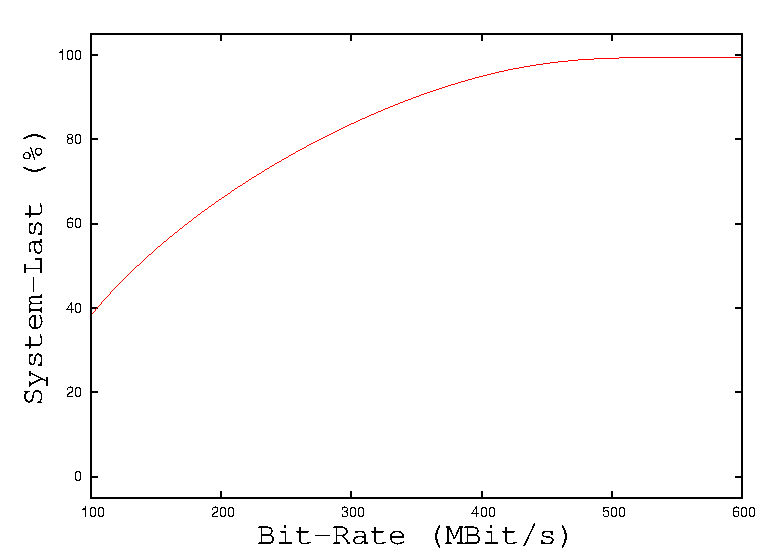
\includegraphics [width=0.45\textwidth]{plots/sysload_generic_slide}}
	\subfigure{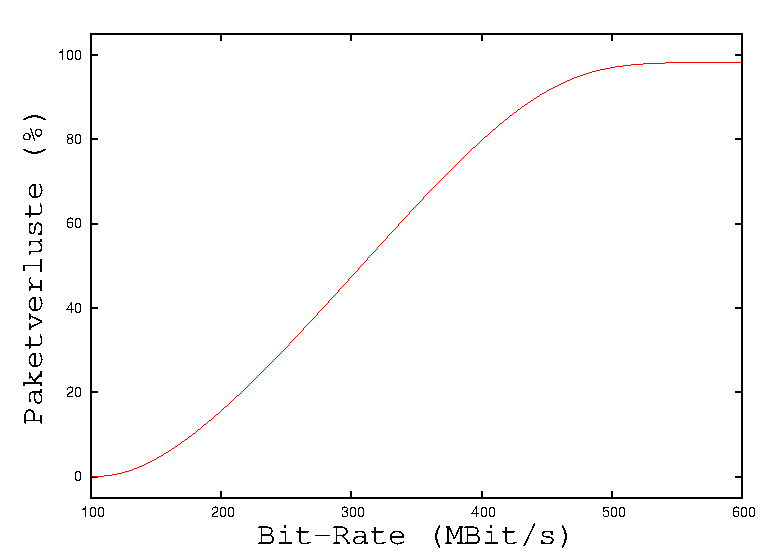
\includegraphics [width=0.45\textwidth]{plots/pktlos_generic_slide}}
	\caption{CPU-load and packet loss by capturing of  64 bytes packets with the standard FreeBSD Capturing software (Bezier curves)}
\end{figure}
\end{frame}

\subsection*{The reason of the Problems}
%%%%%%%%%%%%%%%%%%%%%%%%%%%%%%%%%%%%%%%%%%%%%%%%%%%%%%%%%%%%%%%%%%%
\begin{frame}
\frametitle{The reason of the Problems}
\textbf{Inefficiency of  capturing software}\newline
\begin{itemize}
	\item To many "`expensive"' operations in terms of CPU cycles: 
\begin{itemize}
			\item System calls
			\item Packet copy operations
			\item Memory allocations
			\item etc\ldots\newline
\end{itemize}
\begin{small}
	\item [$\Rightarrow$] may be the capturing software for FreeBSD was
		developed at a time when  network data-rates were low enough relative
		to hardware processing resources such that capturing loss problems did
		not arise.
\end{small}
\end{itemize}
\end{frame}

\subsection*{Goal of the Project}
%%%%%%%%%%%%%%%%%%%%%%%%%%%%%%%%%%%%%%%%%%%%%%%%%%%%%%%%%%%%%%%%%%%
\begin{frame}
\frametitle{Goal of the project}
%\begin{large}
\textbf{What is our goal ?}
%\end{large}
\begin{itemize}
	\item Increase the capturing performance on FreeBSD
		\begin{itemize}
			\item Design and implementation the new capturing software to
				minimize the \textbf{packet loss} and \textbf{cpu load} during capturing. \newline
		\end{itemize}
\end{itemize}
%\begin{large}
\textbf{Conditions:}
%\end{large}
\begin{itemize}
	\item Hardware: \emph{Intel Gigabit Ethernet Adapter}
	\item Software:	\emph{FreeBSD-\textbf{7.x}}
\end{itemize}
\end{frame}

%%%%%%%%%%%%%%%%%%%%%%%%%%%%%%%%%%%%%%%%%%%%%%%%%%%%%%%%%%%%%%%%%%%
\begin{frame}
\frametitle{Approach to a solution}
\begin{itemize}
	\item Eliminating the packet copy operations
		\begin{itemize}
			\item [$\Rightarrow$] by using shared memory buffers (\emph{memory mapping})\newline
		\end{itemize}
	\item Eliminating the memory allocations
		\begin{itemize}
			\item [$\Rightarrow$] by using ring buffers
		\end{itemize}
\end{itemize}
\end{frame}

\section{Background}
%%%%%%%%%%%%%%%%%%%%%%%%%%%%%%%%%%%%%%%%%%%%%%%%%%%%%%%%%%%%%%%%%%%
\begin{frame}
	\begin{center}
	\huge{Background}
	\end{center}
\end{frame}

%%%%%%%%%%%%%%%%%%%%%%%%%%%%%%%%%%%%%%%%%%%%%%%%%%%%%%%%%%%%%%%%%%%
\begin{frame}
\frametitle{Packet Capturing}
\begin{columns}
\column[t]{0.5\textwidth}
\vspace{-15em}
\begin{enumerate}
	\item \textbf{Receiving} network packets
		\begin{itemize}
			\item receive by network adapter
			\item DMA transfer in RAM \newline
		\end{itemize}
	\item \textbf{Filtering} the received packets 
		\begin{itemize}
			\item using software to filter the traffic (e.g. \emph{BPF})\newline
		\end{itemize}
	\item \textbf{Storing} to the hard drive
		\begin{itemize}
			\item due to a system call (\emph{write()})
		\end{itemize}
\end{enumerate}
\column[t]{0.5\textwidth}
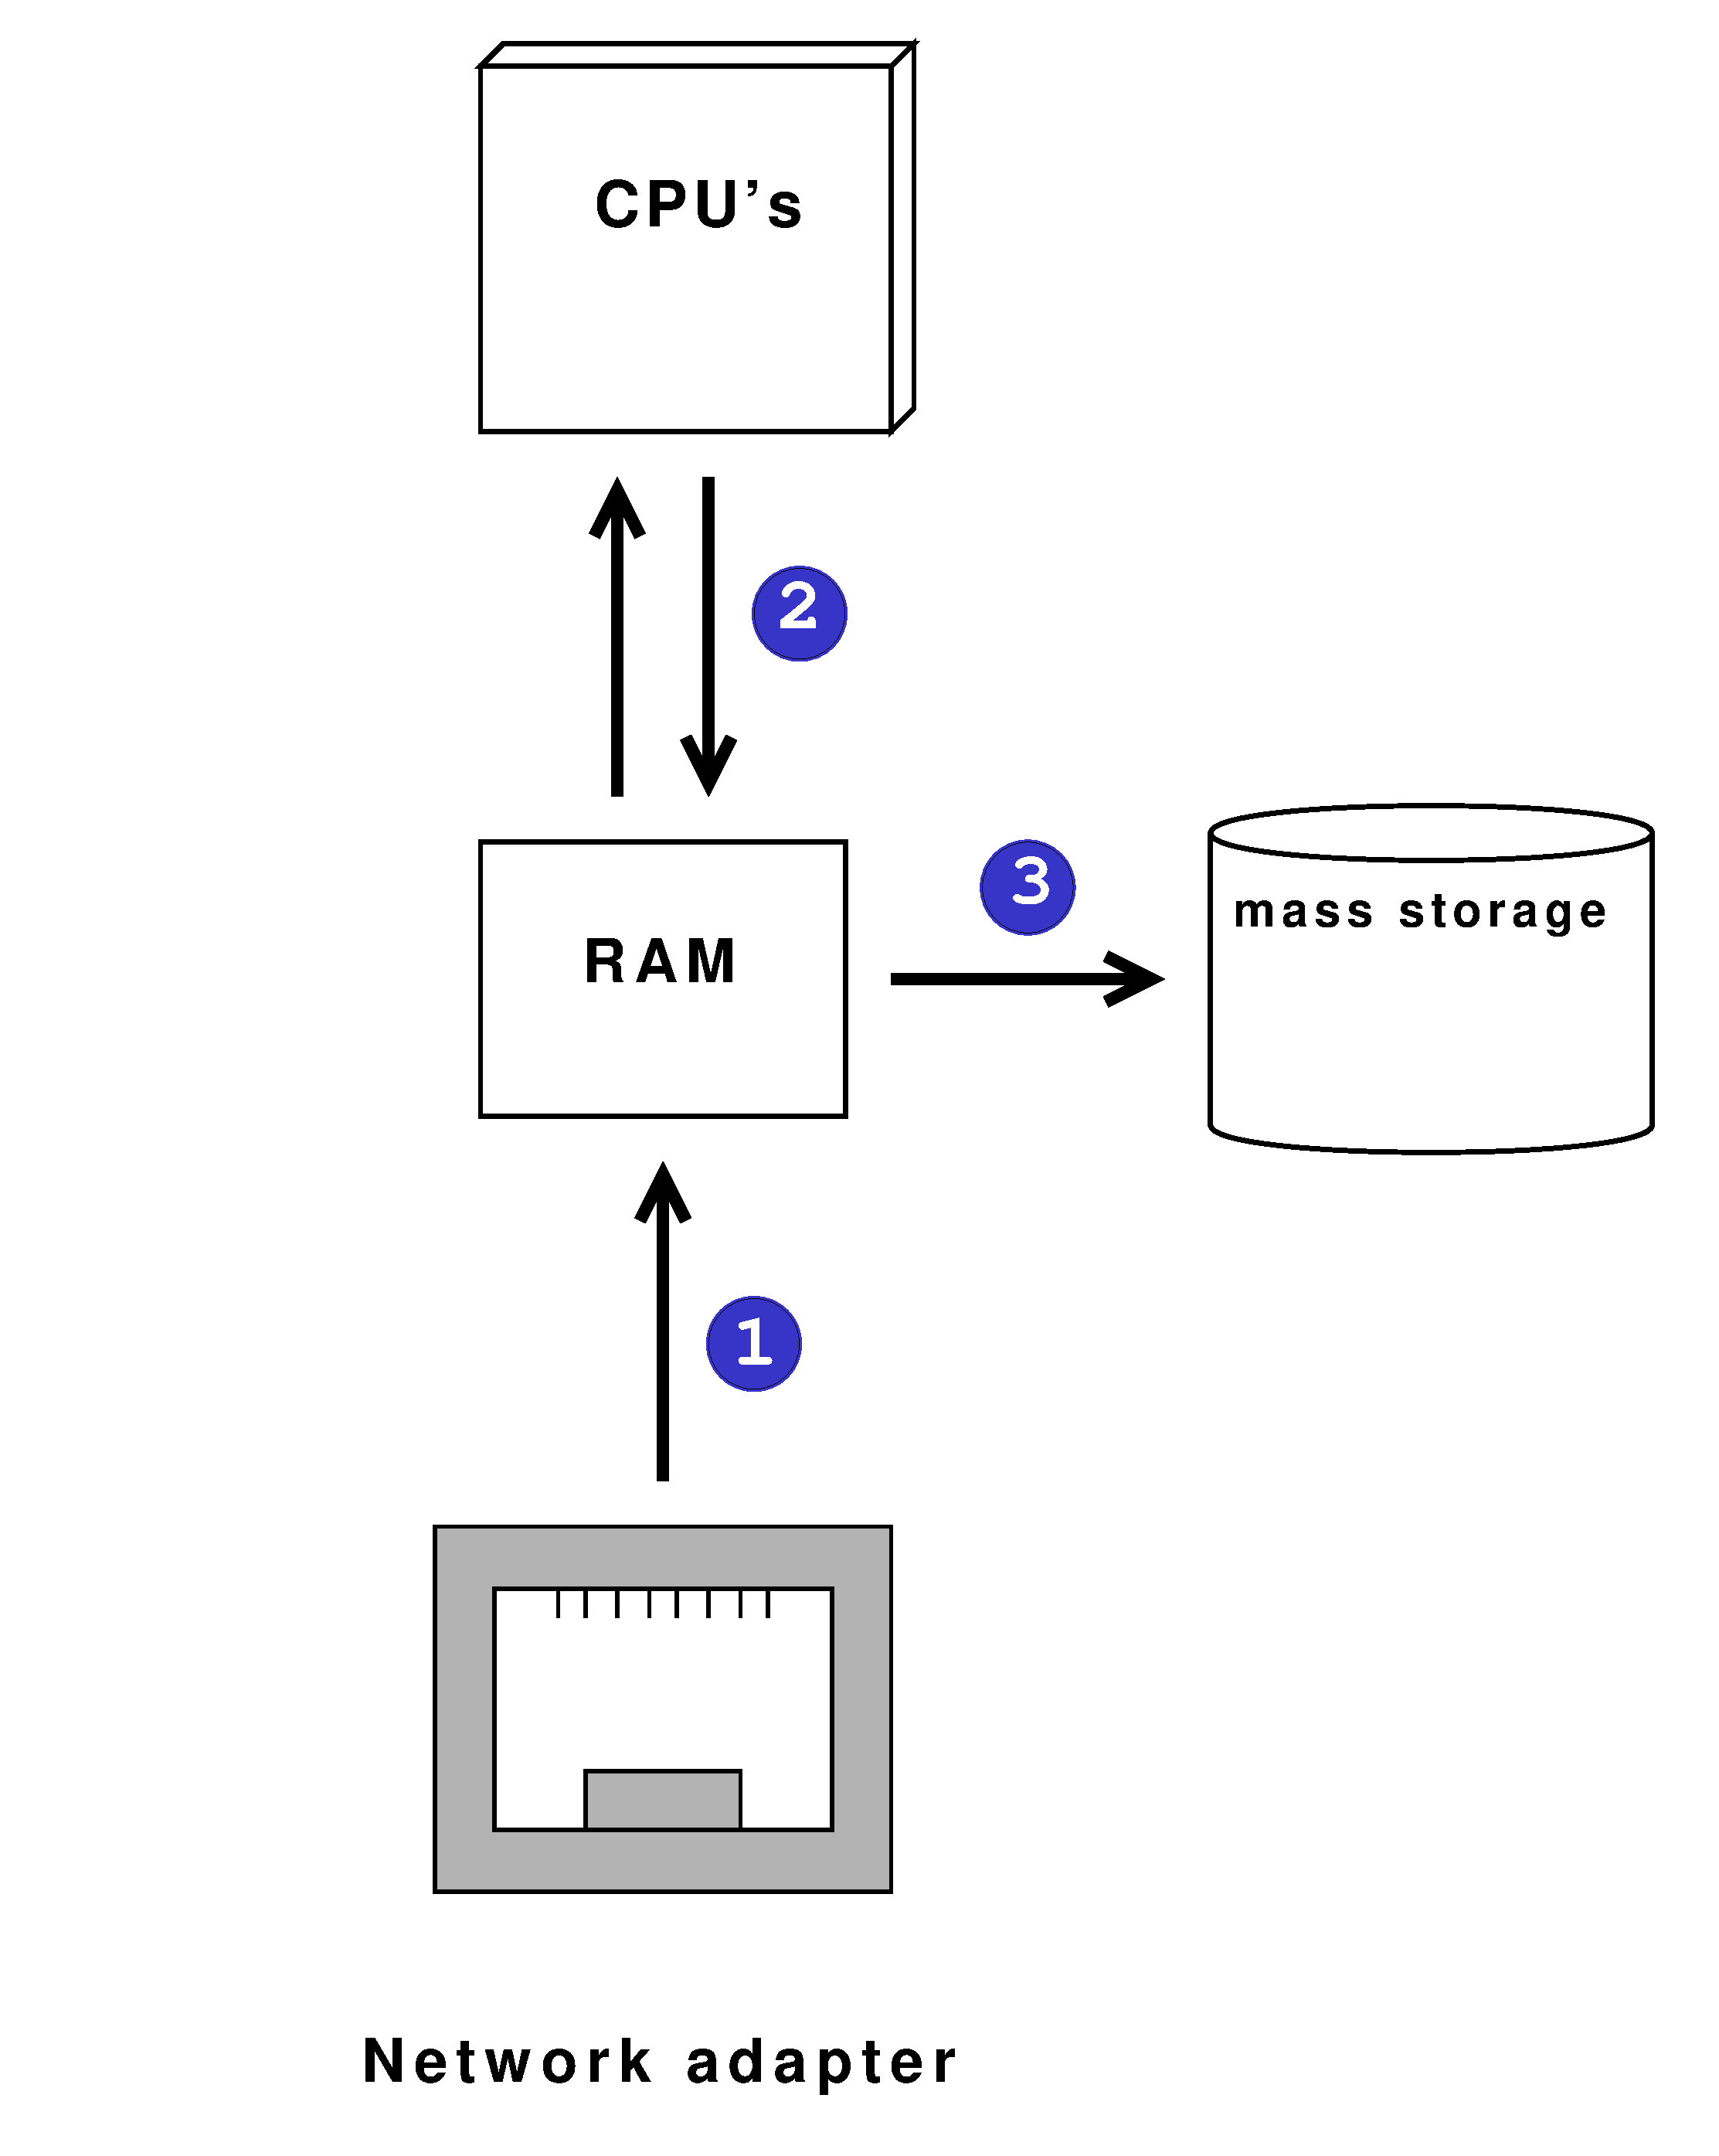
\includegraphics [width=0.82\textwidth, keepaspectratio]{pics/HardwareView}
\end{columns}
\end{frame}

%%%%%%%%%%%%%%%%%%%%%%%%%%%%%%%%%%%%%%%%%%%%%%%%%%%%%%%%%%%%%%%%%%%
\begin{frame}
\frametitle{FreeBSD Packet Capturing Stack}
\begin{itemize}
	\item \textbf{Network driver}
		\begin{itemize}
			\item Receiving the packets\newline
		\end{itemize}
	\item \textbf{Berkley Packet Filter} (BPF)
		\begin{itemize}
			\item Filtering the packets\newline
		\end{itemize}
	\item \textbf{Userspace application}
		\begin{itemize}
			\item Access to the received packets
			\item Initiates:
				\begin{itemize}
					\item Storing of packets to hard drive
					\item Output packet information to the terminal
				\end{itemize}
		\end{itemize}
\end{itemize}
\end{frame}

\subsection*{Capturing}
%%%%%%%%%%%%%%%%%%%%%%%%%%%%%%%%%%%%%%%%%%%%%%%%%%%%%%%%%%%%%%%%%%%
\begin{frame}
	\begin{center}
	\huge{The way of the packet during capturing}
	\end{center}
\end{frame}


%%%%%%%%%%%%%%%%%%%%%%%%%%%%%%%%%%%%%%%%%%%%%%%%%%%%%%%%%%%%%%%%%%%
\begin{frame}
\frametitle{FreeBSD-7 Packet Capturing Stack}
\begin{columns}
\column[t]{0.5\textwidth}
\vspace{0em}
\begin{itemize}
\item <7-> Access packets
	\begin{itemize}
		\item <7->due to the \emph{read}-Syscall
		\item <7->BPF-Buffer $\Rightarrow$ 	User-Buffer
	\end{itemize}
\item <5-> Packet filtering
	\begin{itemize}
		\item <5->Filtering the packets 
		\item <6->Packet-Buffer $\Rightarrow$ BPF-Buffer
	\end{itemize}
\item <4-> Interrupt Service Routine
\item <3-> Interrupt
\item <2-> DMA-Transfer
	\begin{itemize}
		\item <2->Adapter-FIFO $\Rightarrow$ Packet-Buffer
	\end{itemize}
\end{itemize}
\column[t]{0.5\textwidth}
\vspace{-2em}
\begin{figure}
	\only<1>{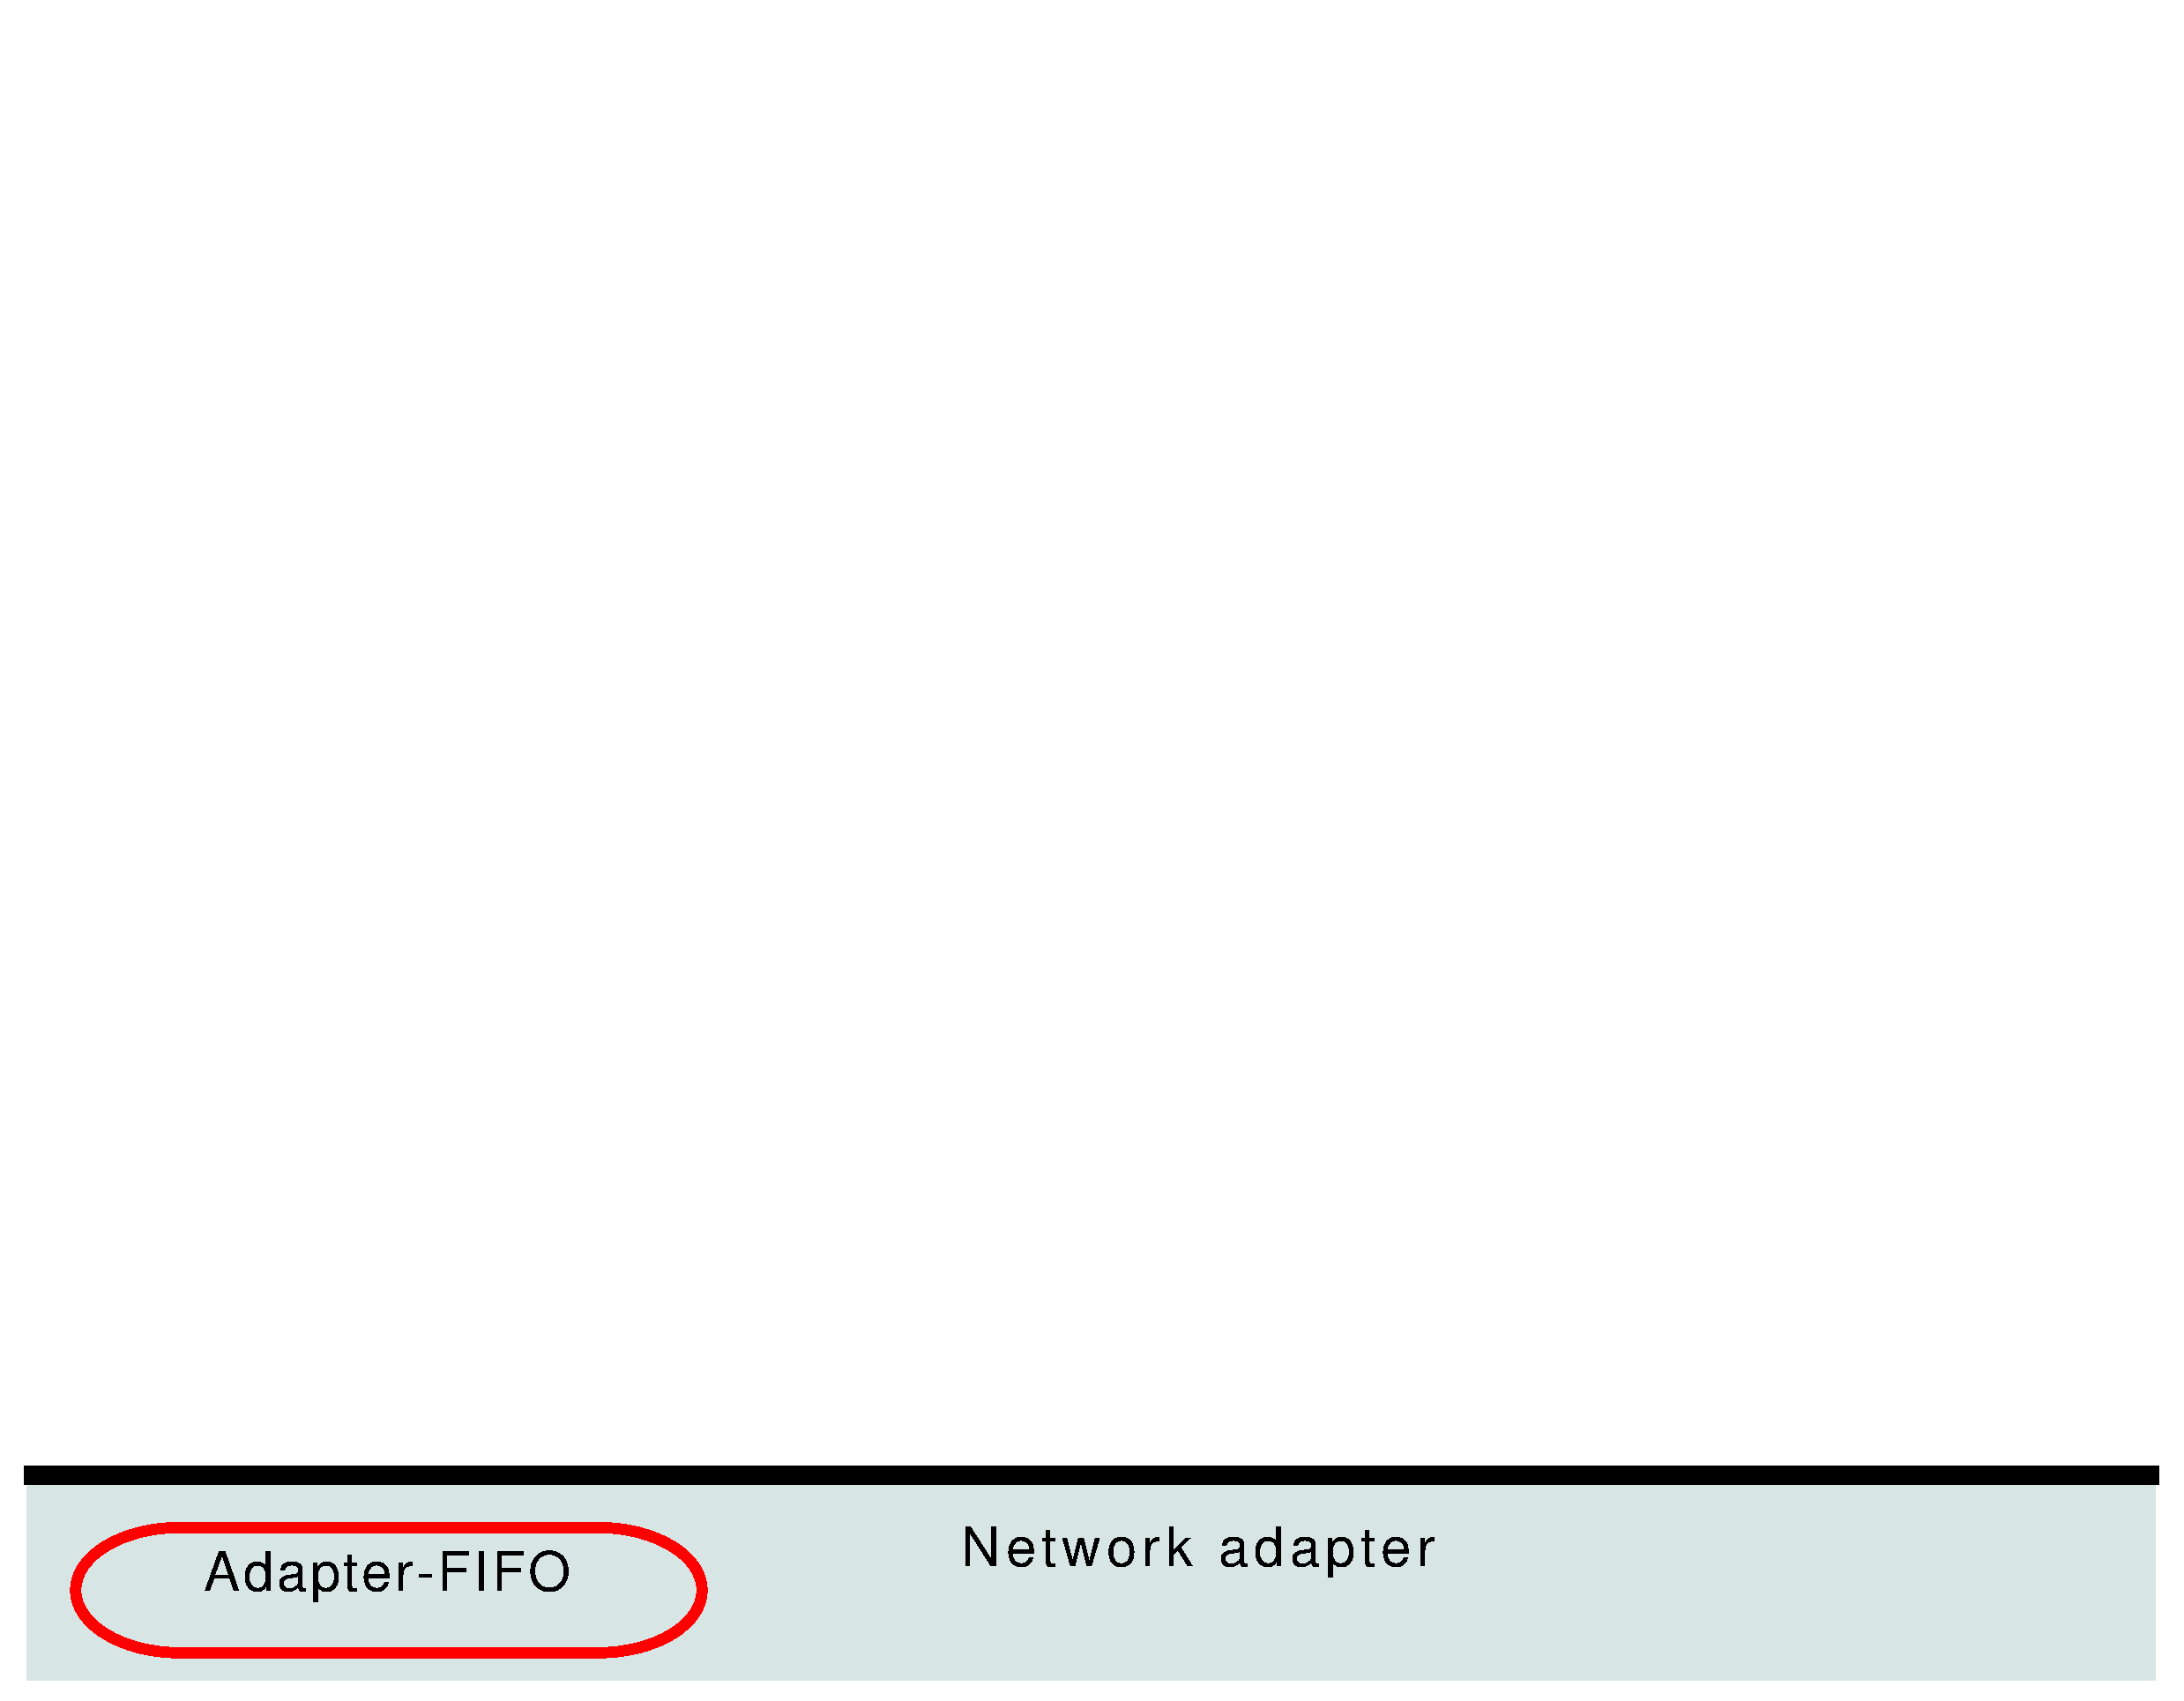
\includegraphics [height=64mm,width=60mm]{pics/3copy_0}}
	\only<2>{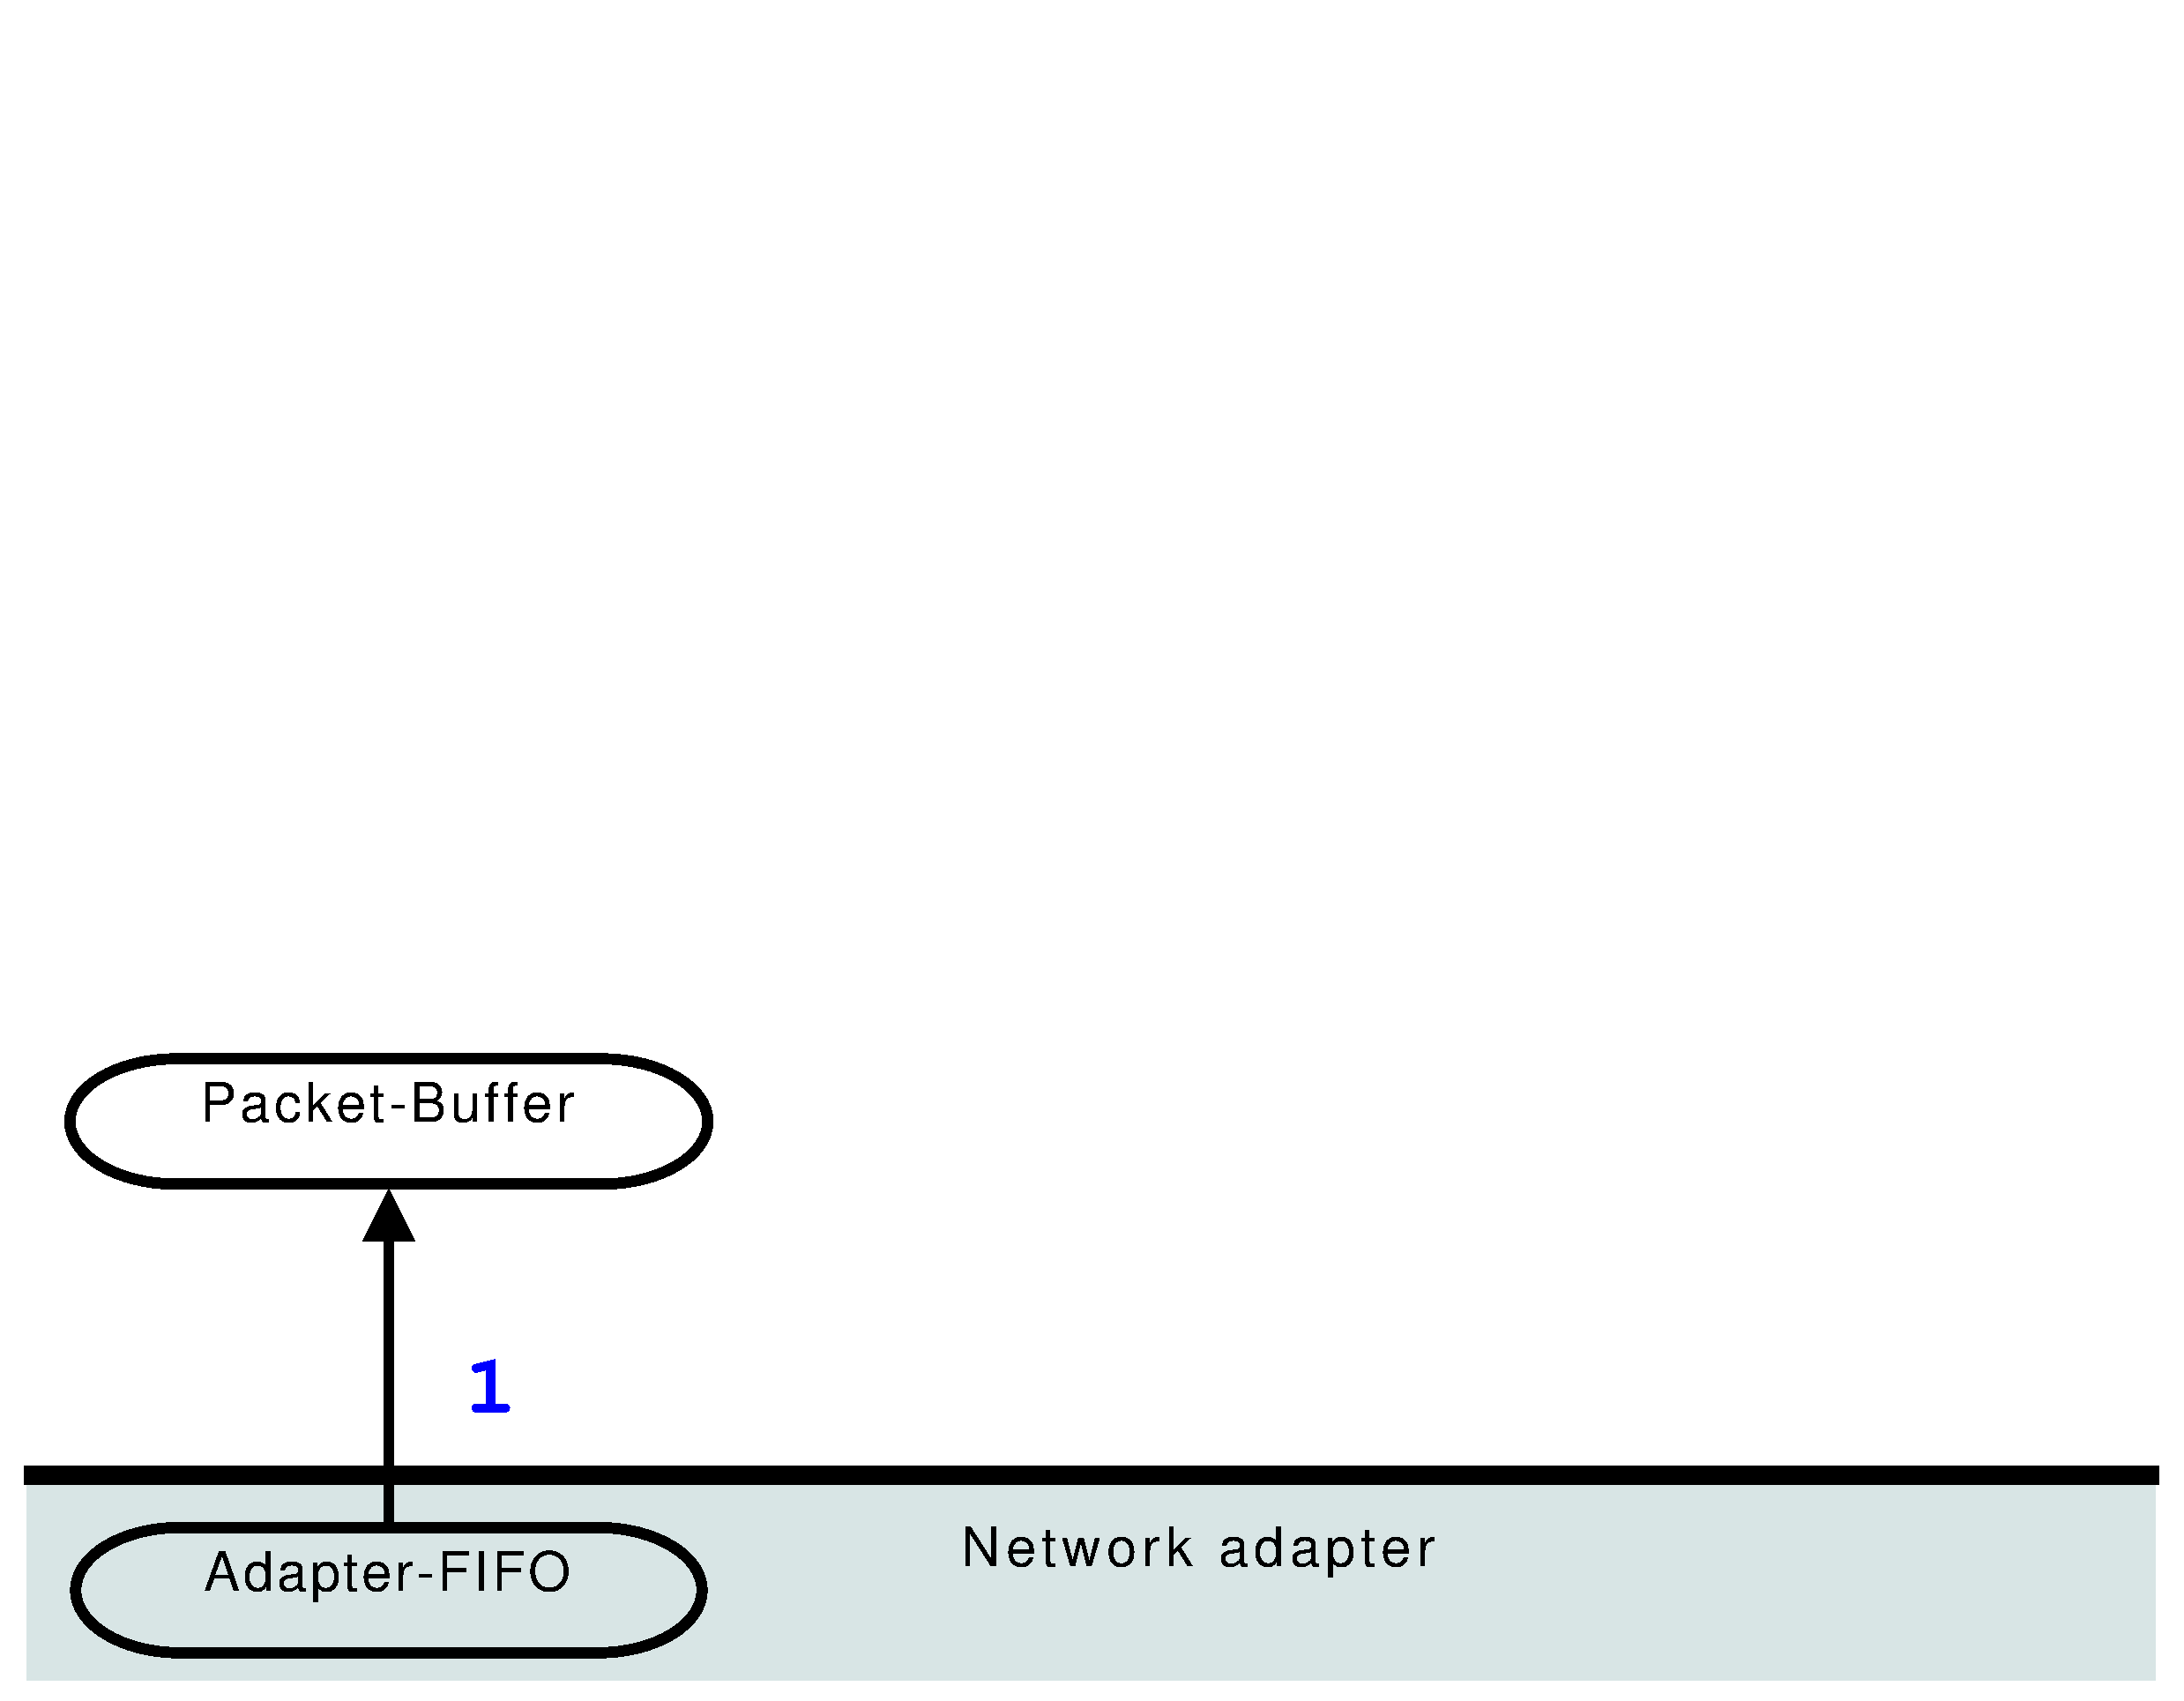
\includegraphics [height=64mm,width=60mm]{pics/3copy_0.5.eps}}
	\only<3>{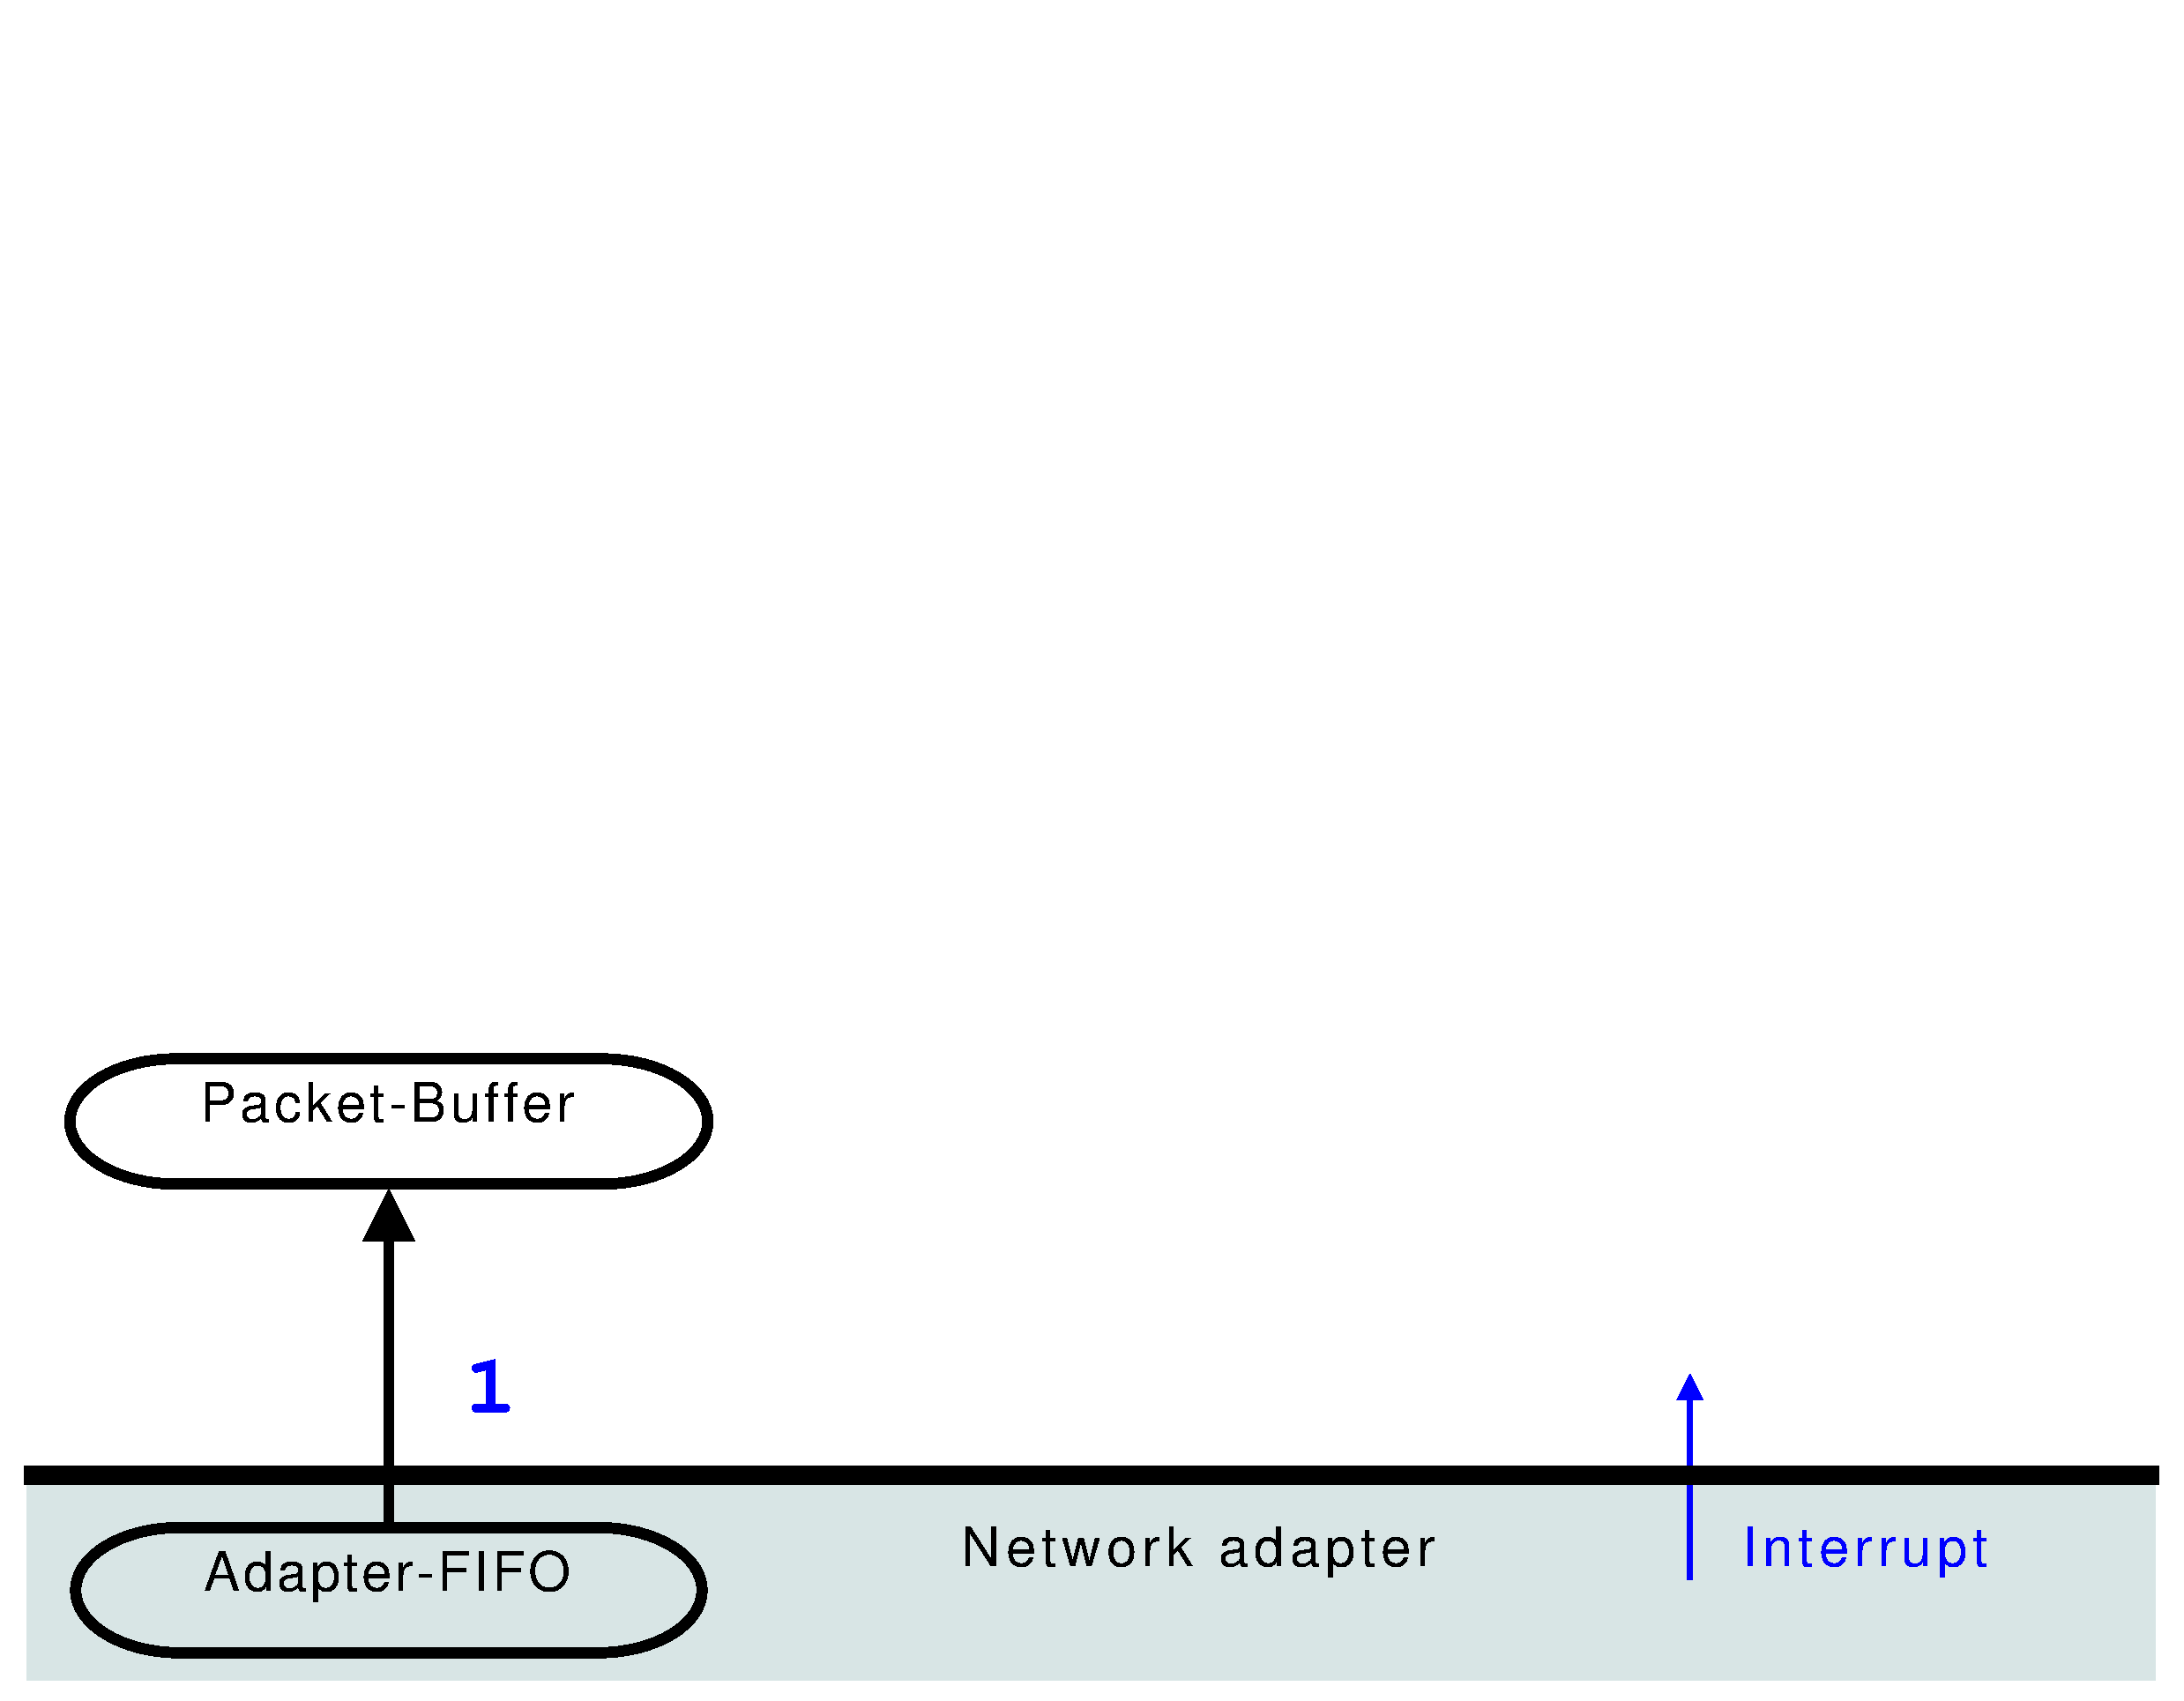
\includegraphics [height=64mm,width=60mm]{pics/3copy_0.7.eps}}
	\only<4>{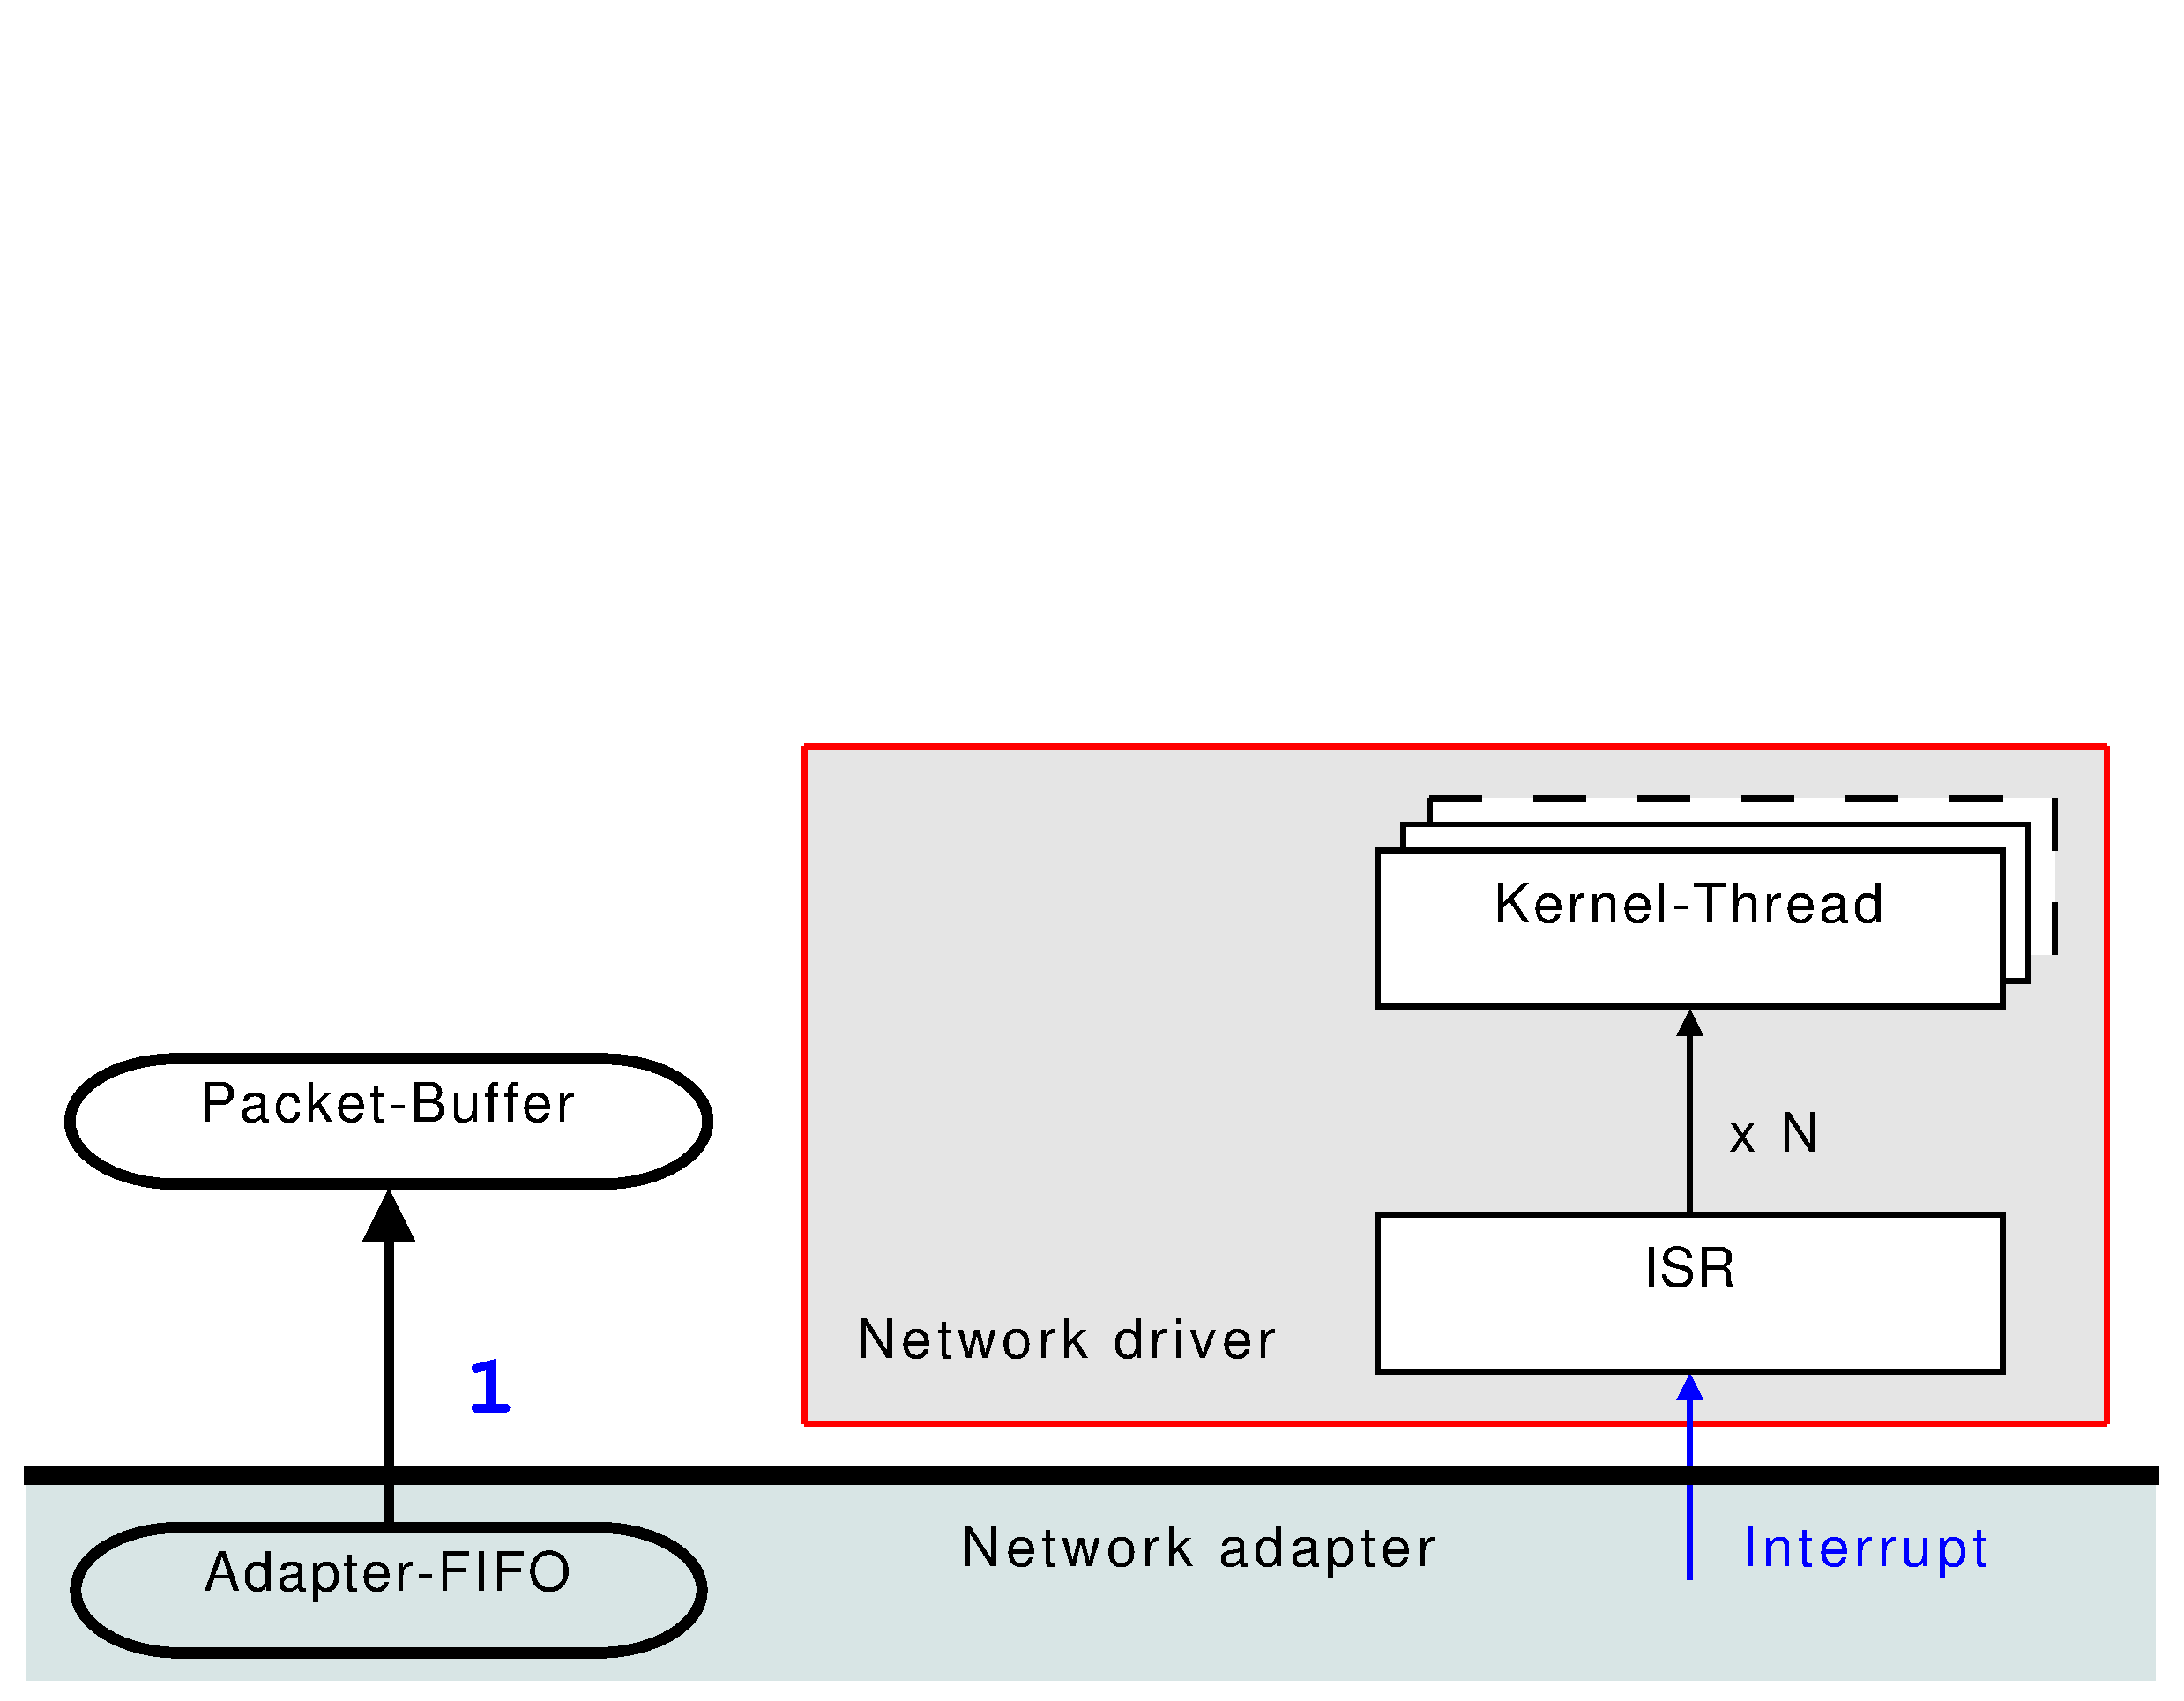
\includegraphics [height=64mm,width=60mm]{pics/3copy_1}}
	\only<5>{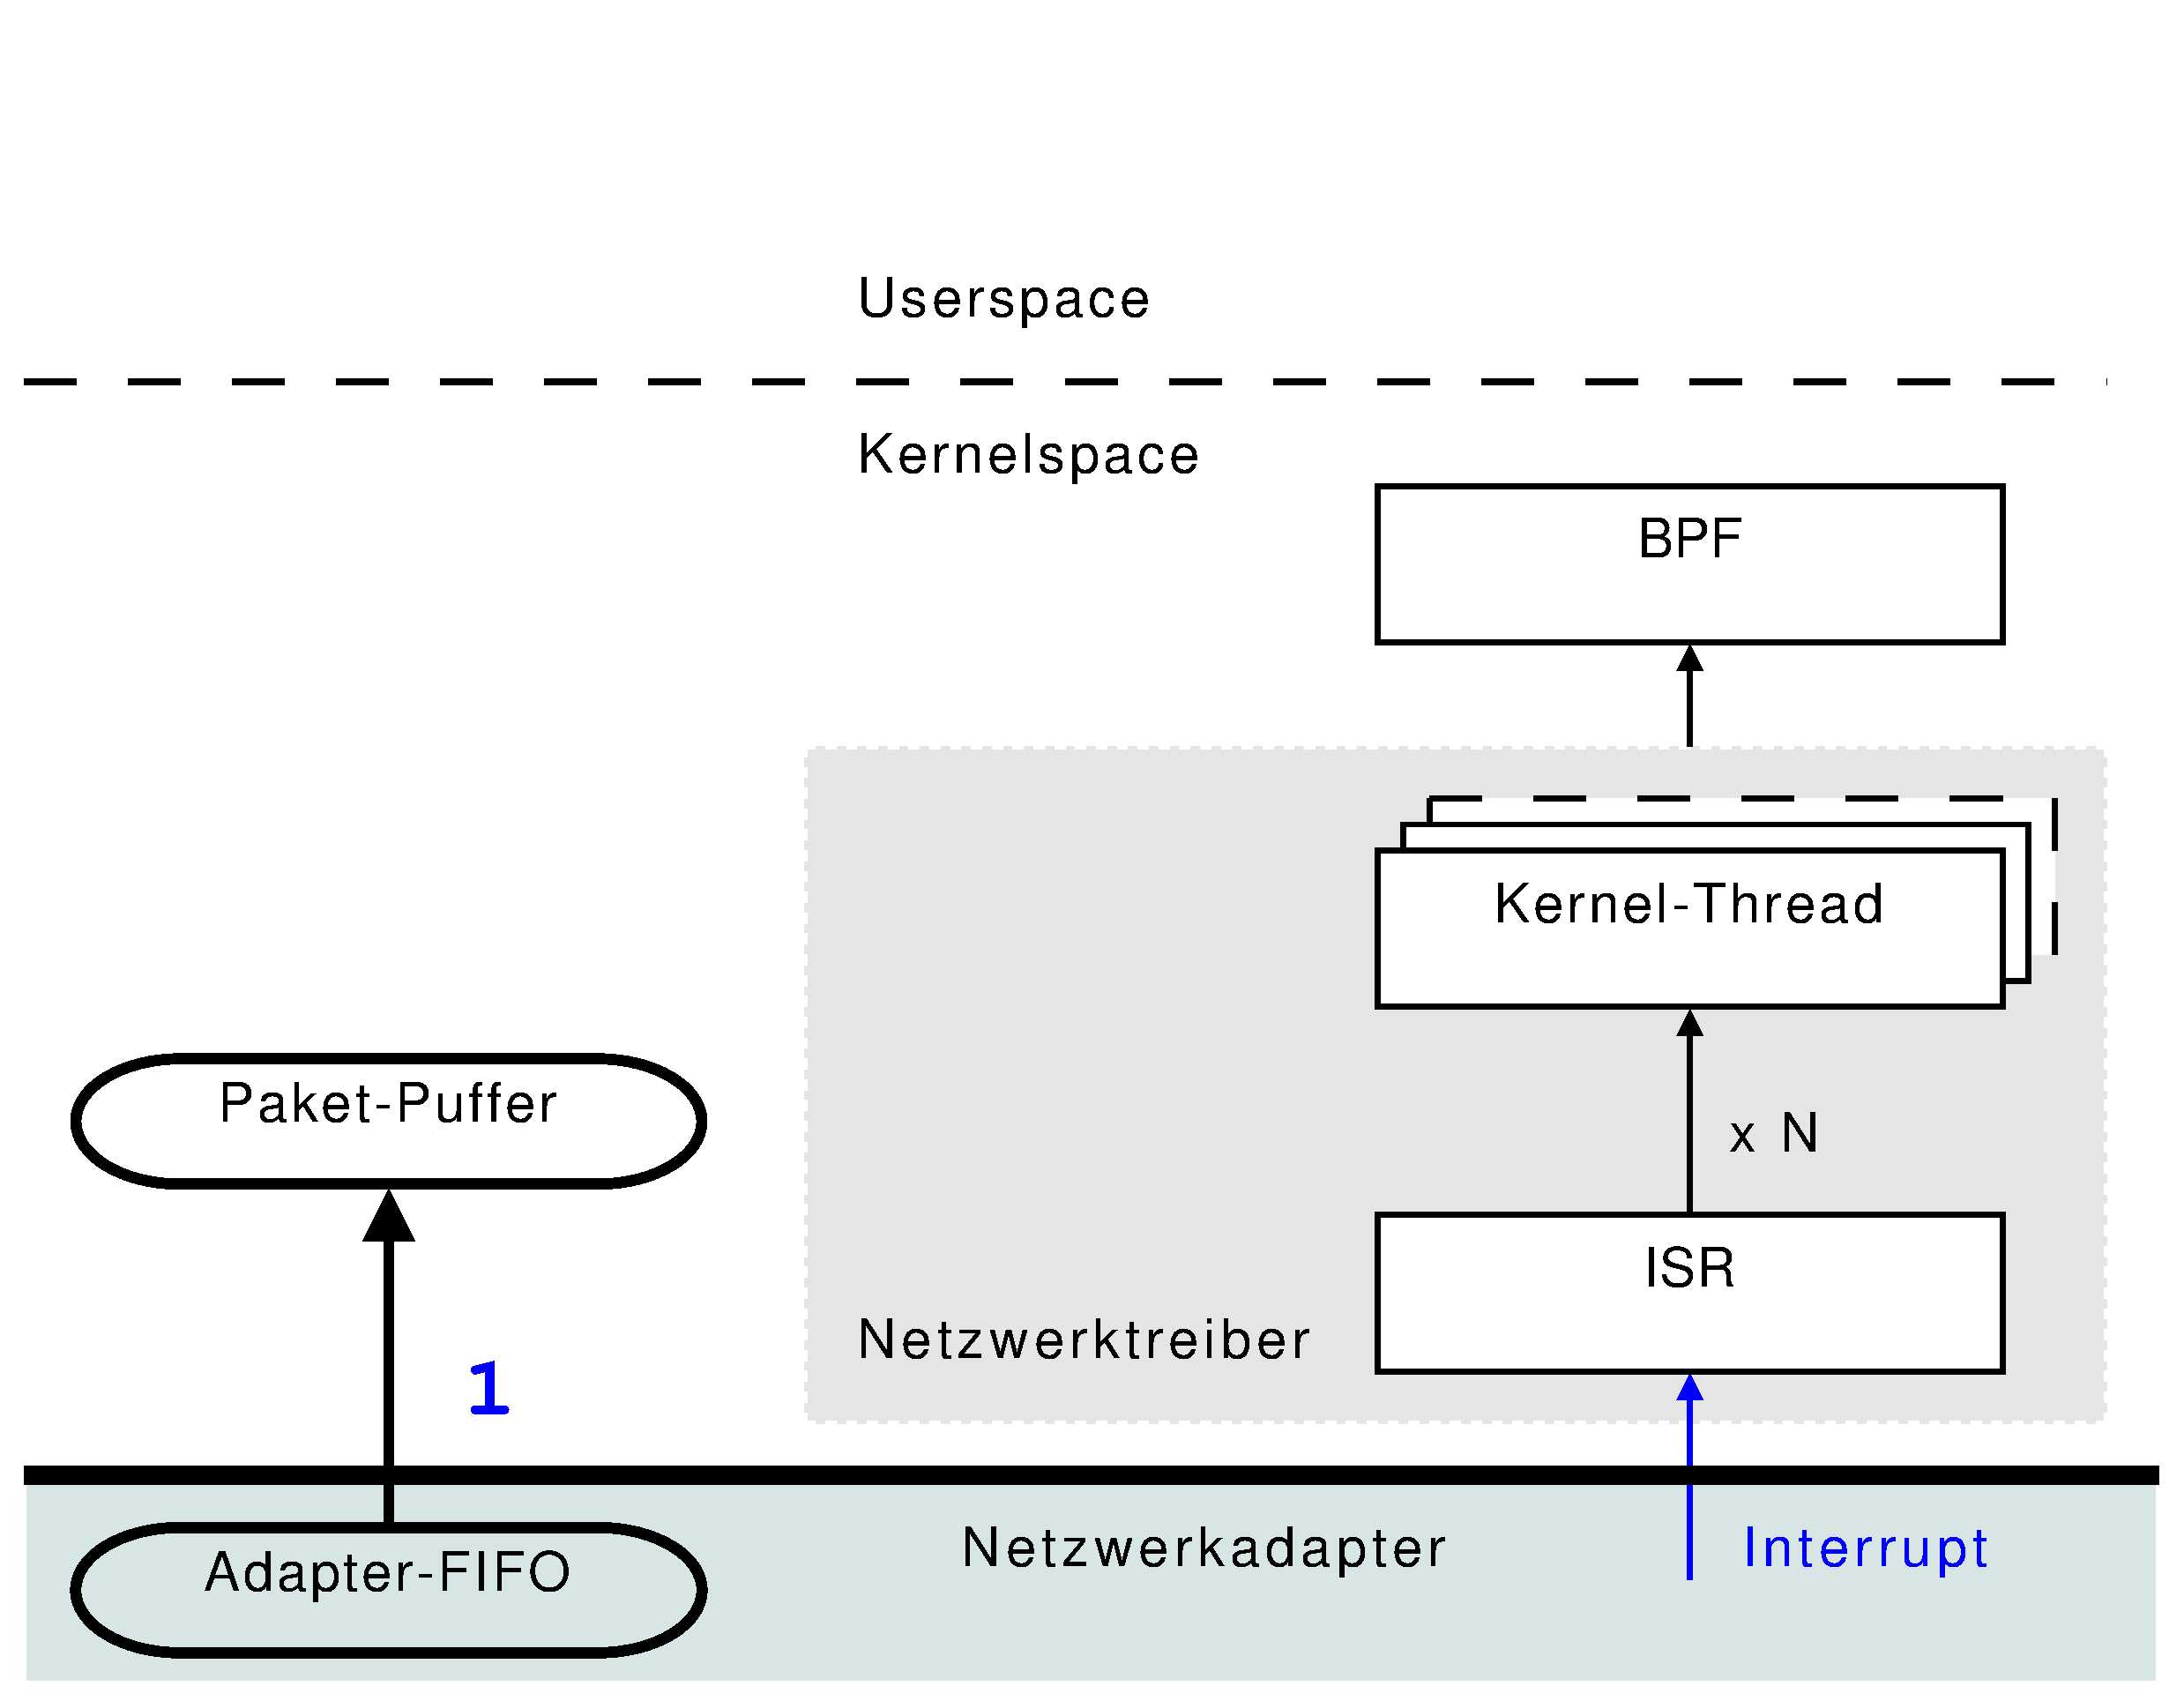
\includegraphics [height=64mm,width=60mm]{pics/3copy_1_1}}
	\only<6>{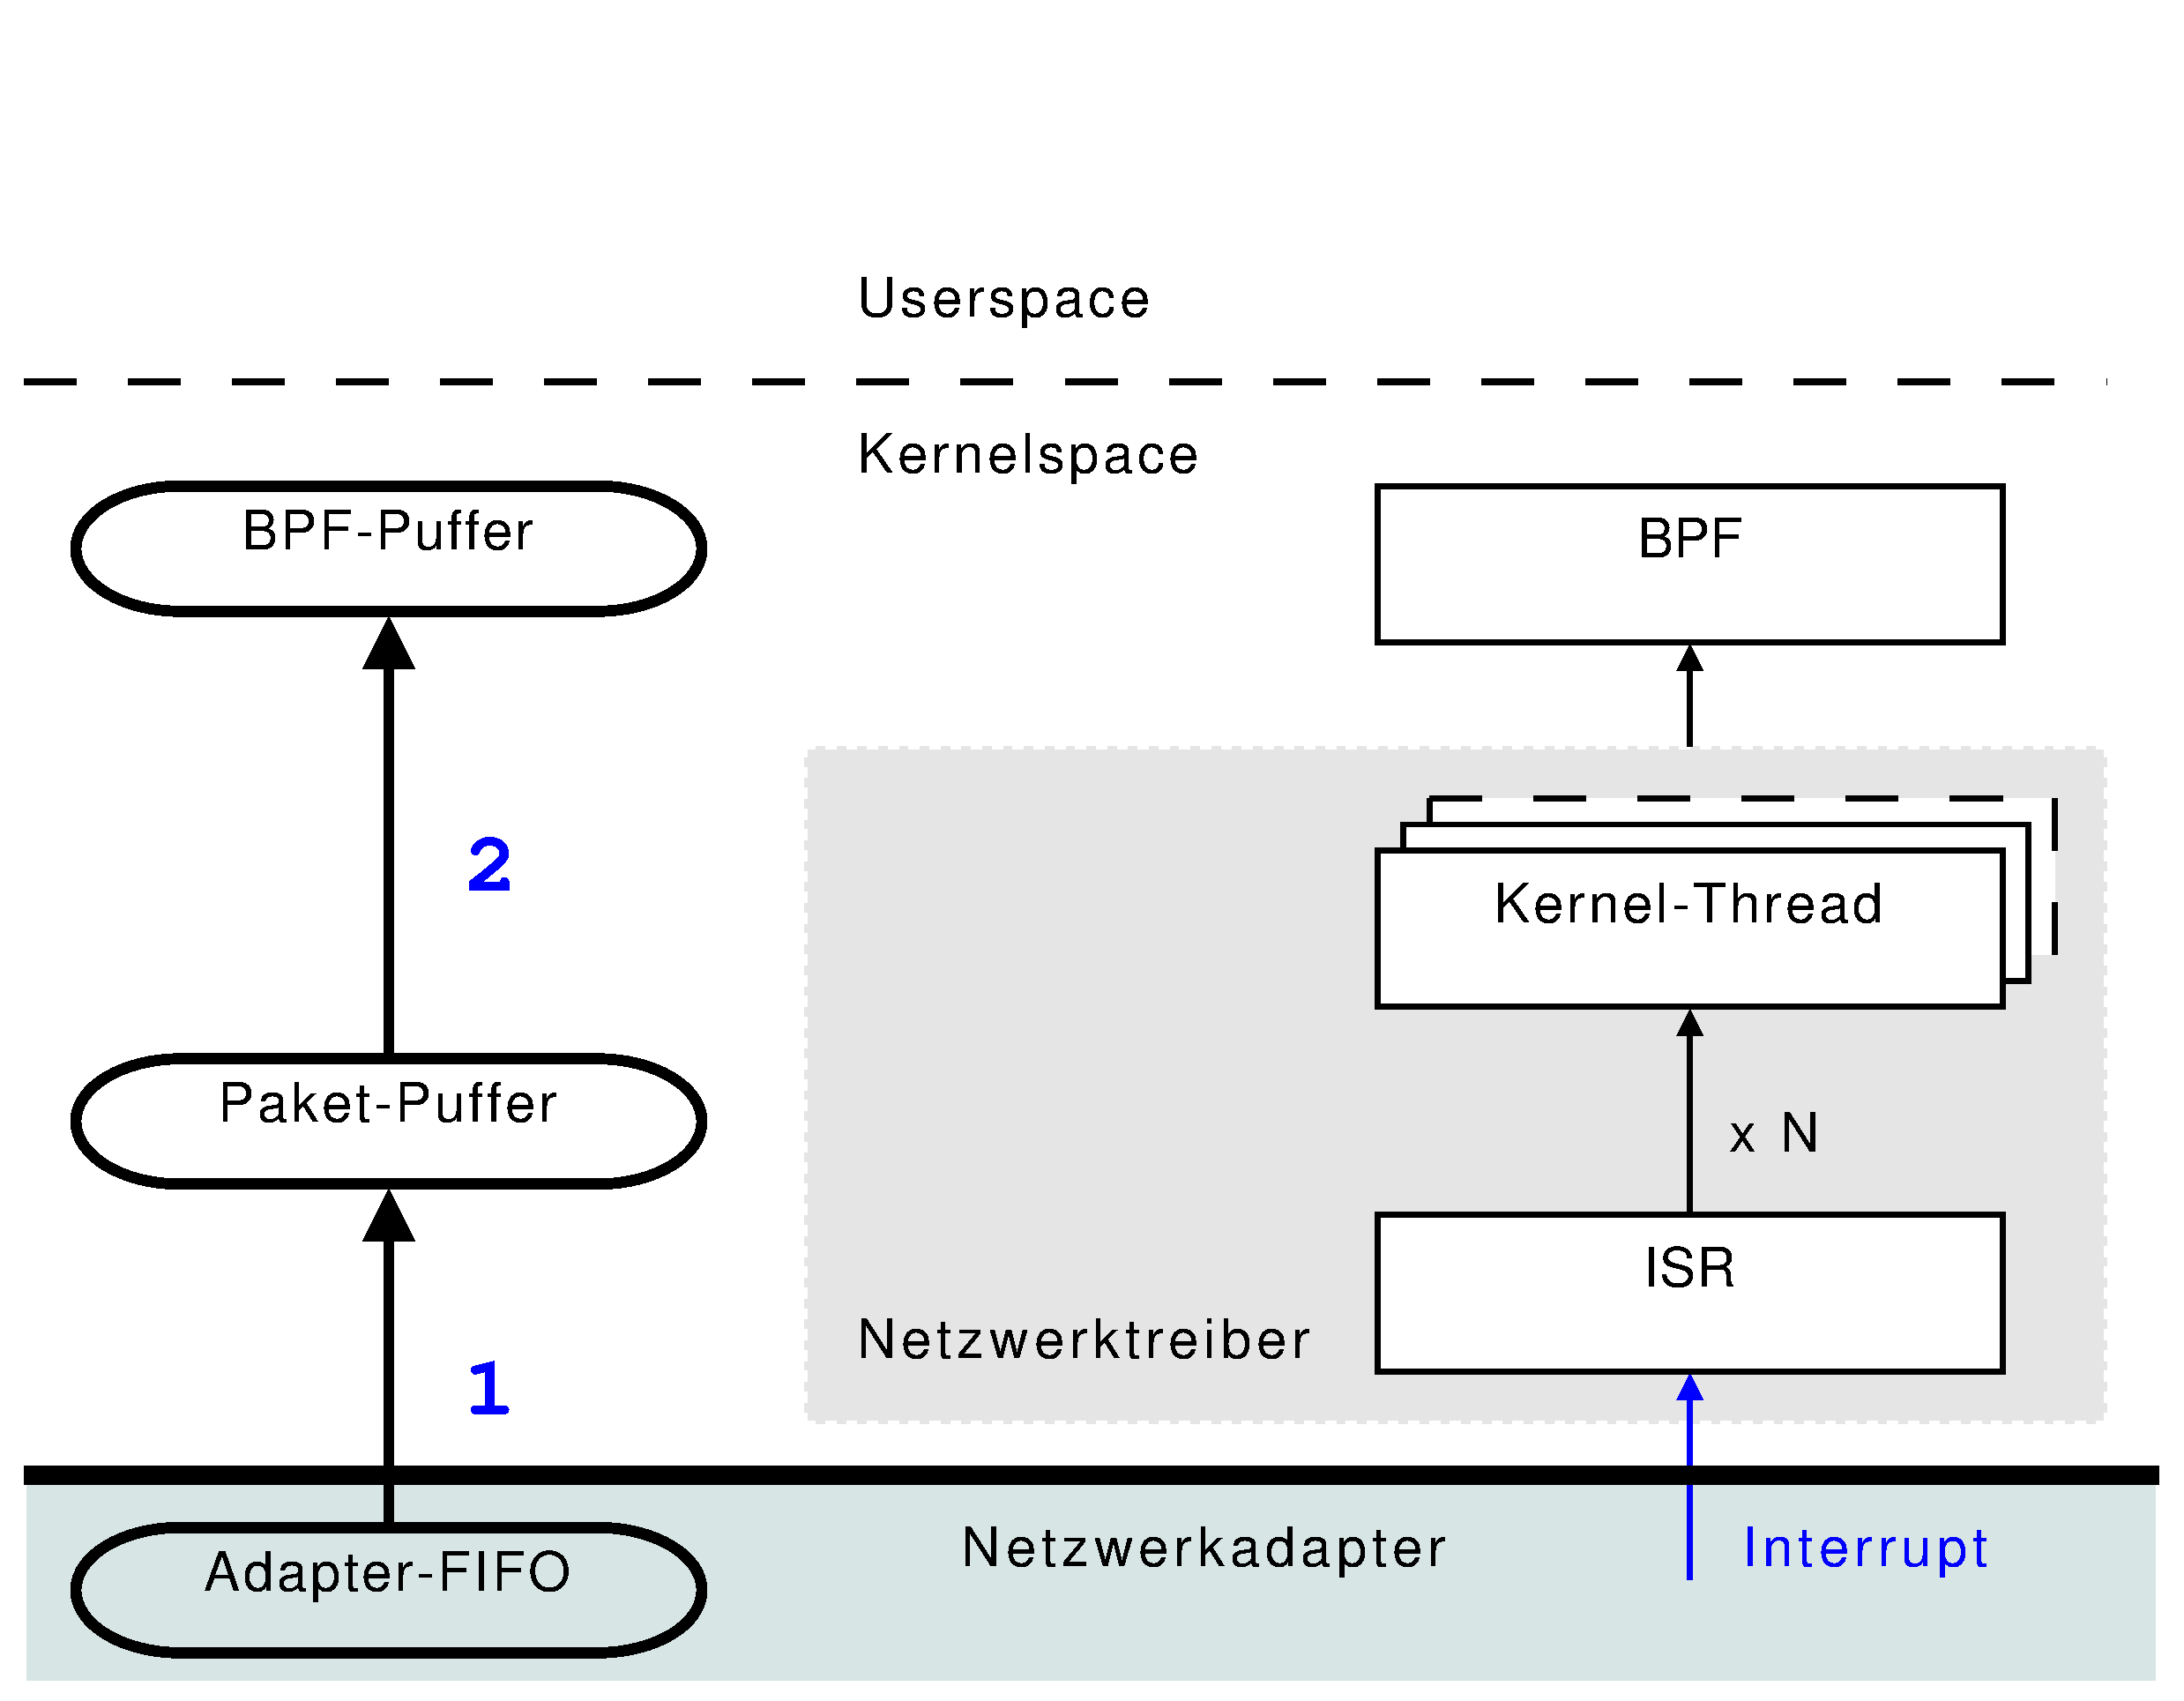
\includegraphics [height=64mm,width=60mm]{pics/3copy_2}}
	\only<7>{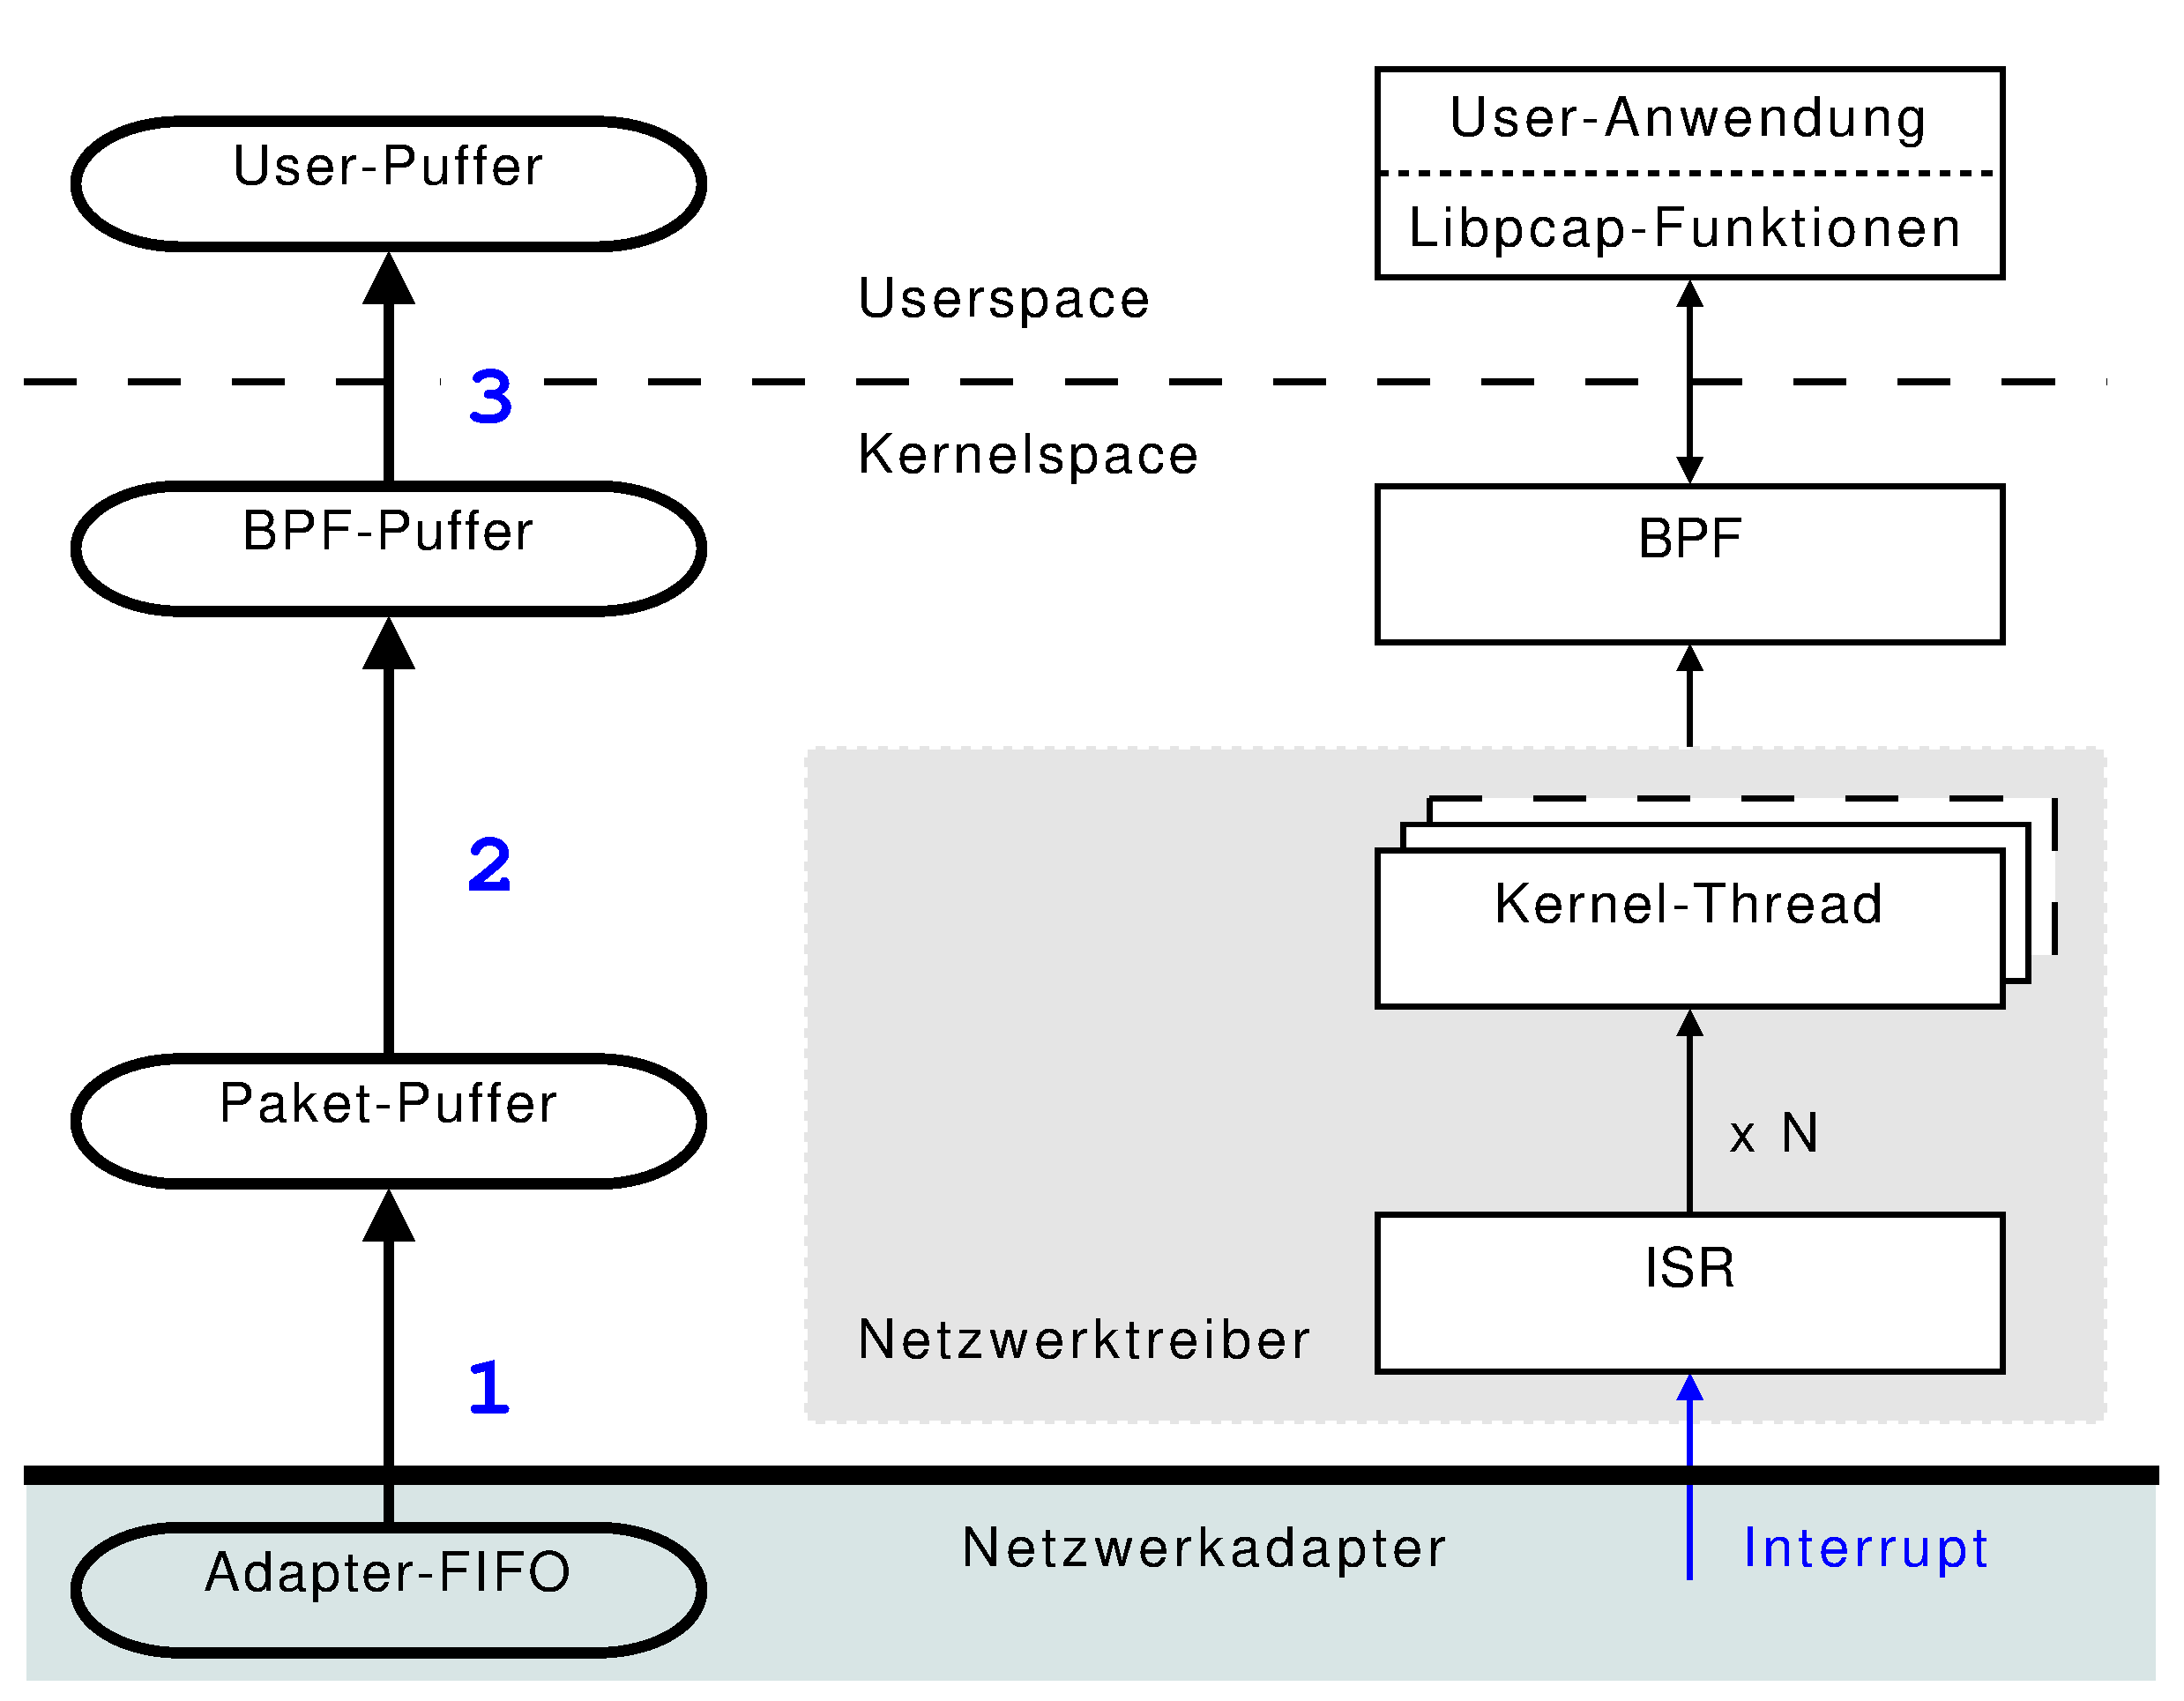
\includegraphics [height=64mm,width=60mm]{pics/3copy_3}}
\end{figure}
\end{columns}
\end{frame}


%%%%%%%%%%%%%%%%%%%%%%%%%%%%%%%%%%%%%%%%%%%%%%%%%%%%%%%%%%%%%%%%%%%

%	Description of Task, Goal, Aufgabenstellung
\section{Approach to a solution}

\begin{frame}
	\begin{center}
	\huge{Approach to a solution}
	\end{center}
\end{frame}


\subsection*{Capturing stacks}
%%%%%%%%%%%%%%%%%%%%%%%%%%%%%%%%%%%%%%%%%%%%%%%%%%%%%%%%%%%%%%%%%%%
\begin{frame}
\frametitle{Packet Capturing Stacks}
\textbf{ringmap:}
\begin{itemize}
	\item Our new packet capturing stack.
	\item Based on \textbf{generic}-Stack, but "`a little"' changed.\newline
\end{itemize}
\textbf{generic:}
\begin{itemize}
	\item Standard Packet Capturing Stack in FreeBSD-\textbf{7.x}\newline
\end{itemize}
\only<2>{Where the changes are taking place?}
\end{frame}


\subsection*{Changes in generic-Stack}
%%%%%%%%%%%%%%%%%%%%%%%%%%%%%%%%%%%%%%%%%%%%%%%%%%%%%%%%%%%%%%%%%%%
\begin{frame}
\frametitle{What is in generic changed}
\begin{columns}
\column[t]{0.5\textwidth}
\begin{itemize}
	\item <2->Disable TCP/IP-Stack\newline
	\item <3->No optimization for storing the packets\newline
	\item <4->Kernel-Thread, BPF and Libpcap will be optimized\newline
		\begin{itemize}
			\item <4->ISR is not changed
		\end{itemize}
\end{itemize}
\column[t]{0.5\textwidth}
\vspace{-2em}
\only<1>{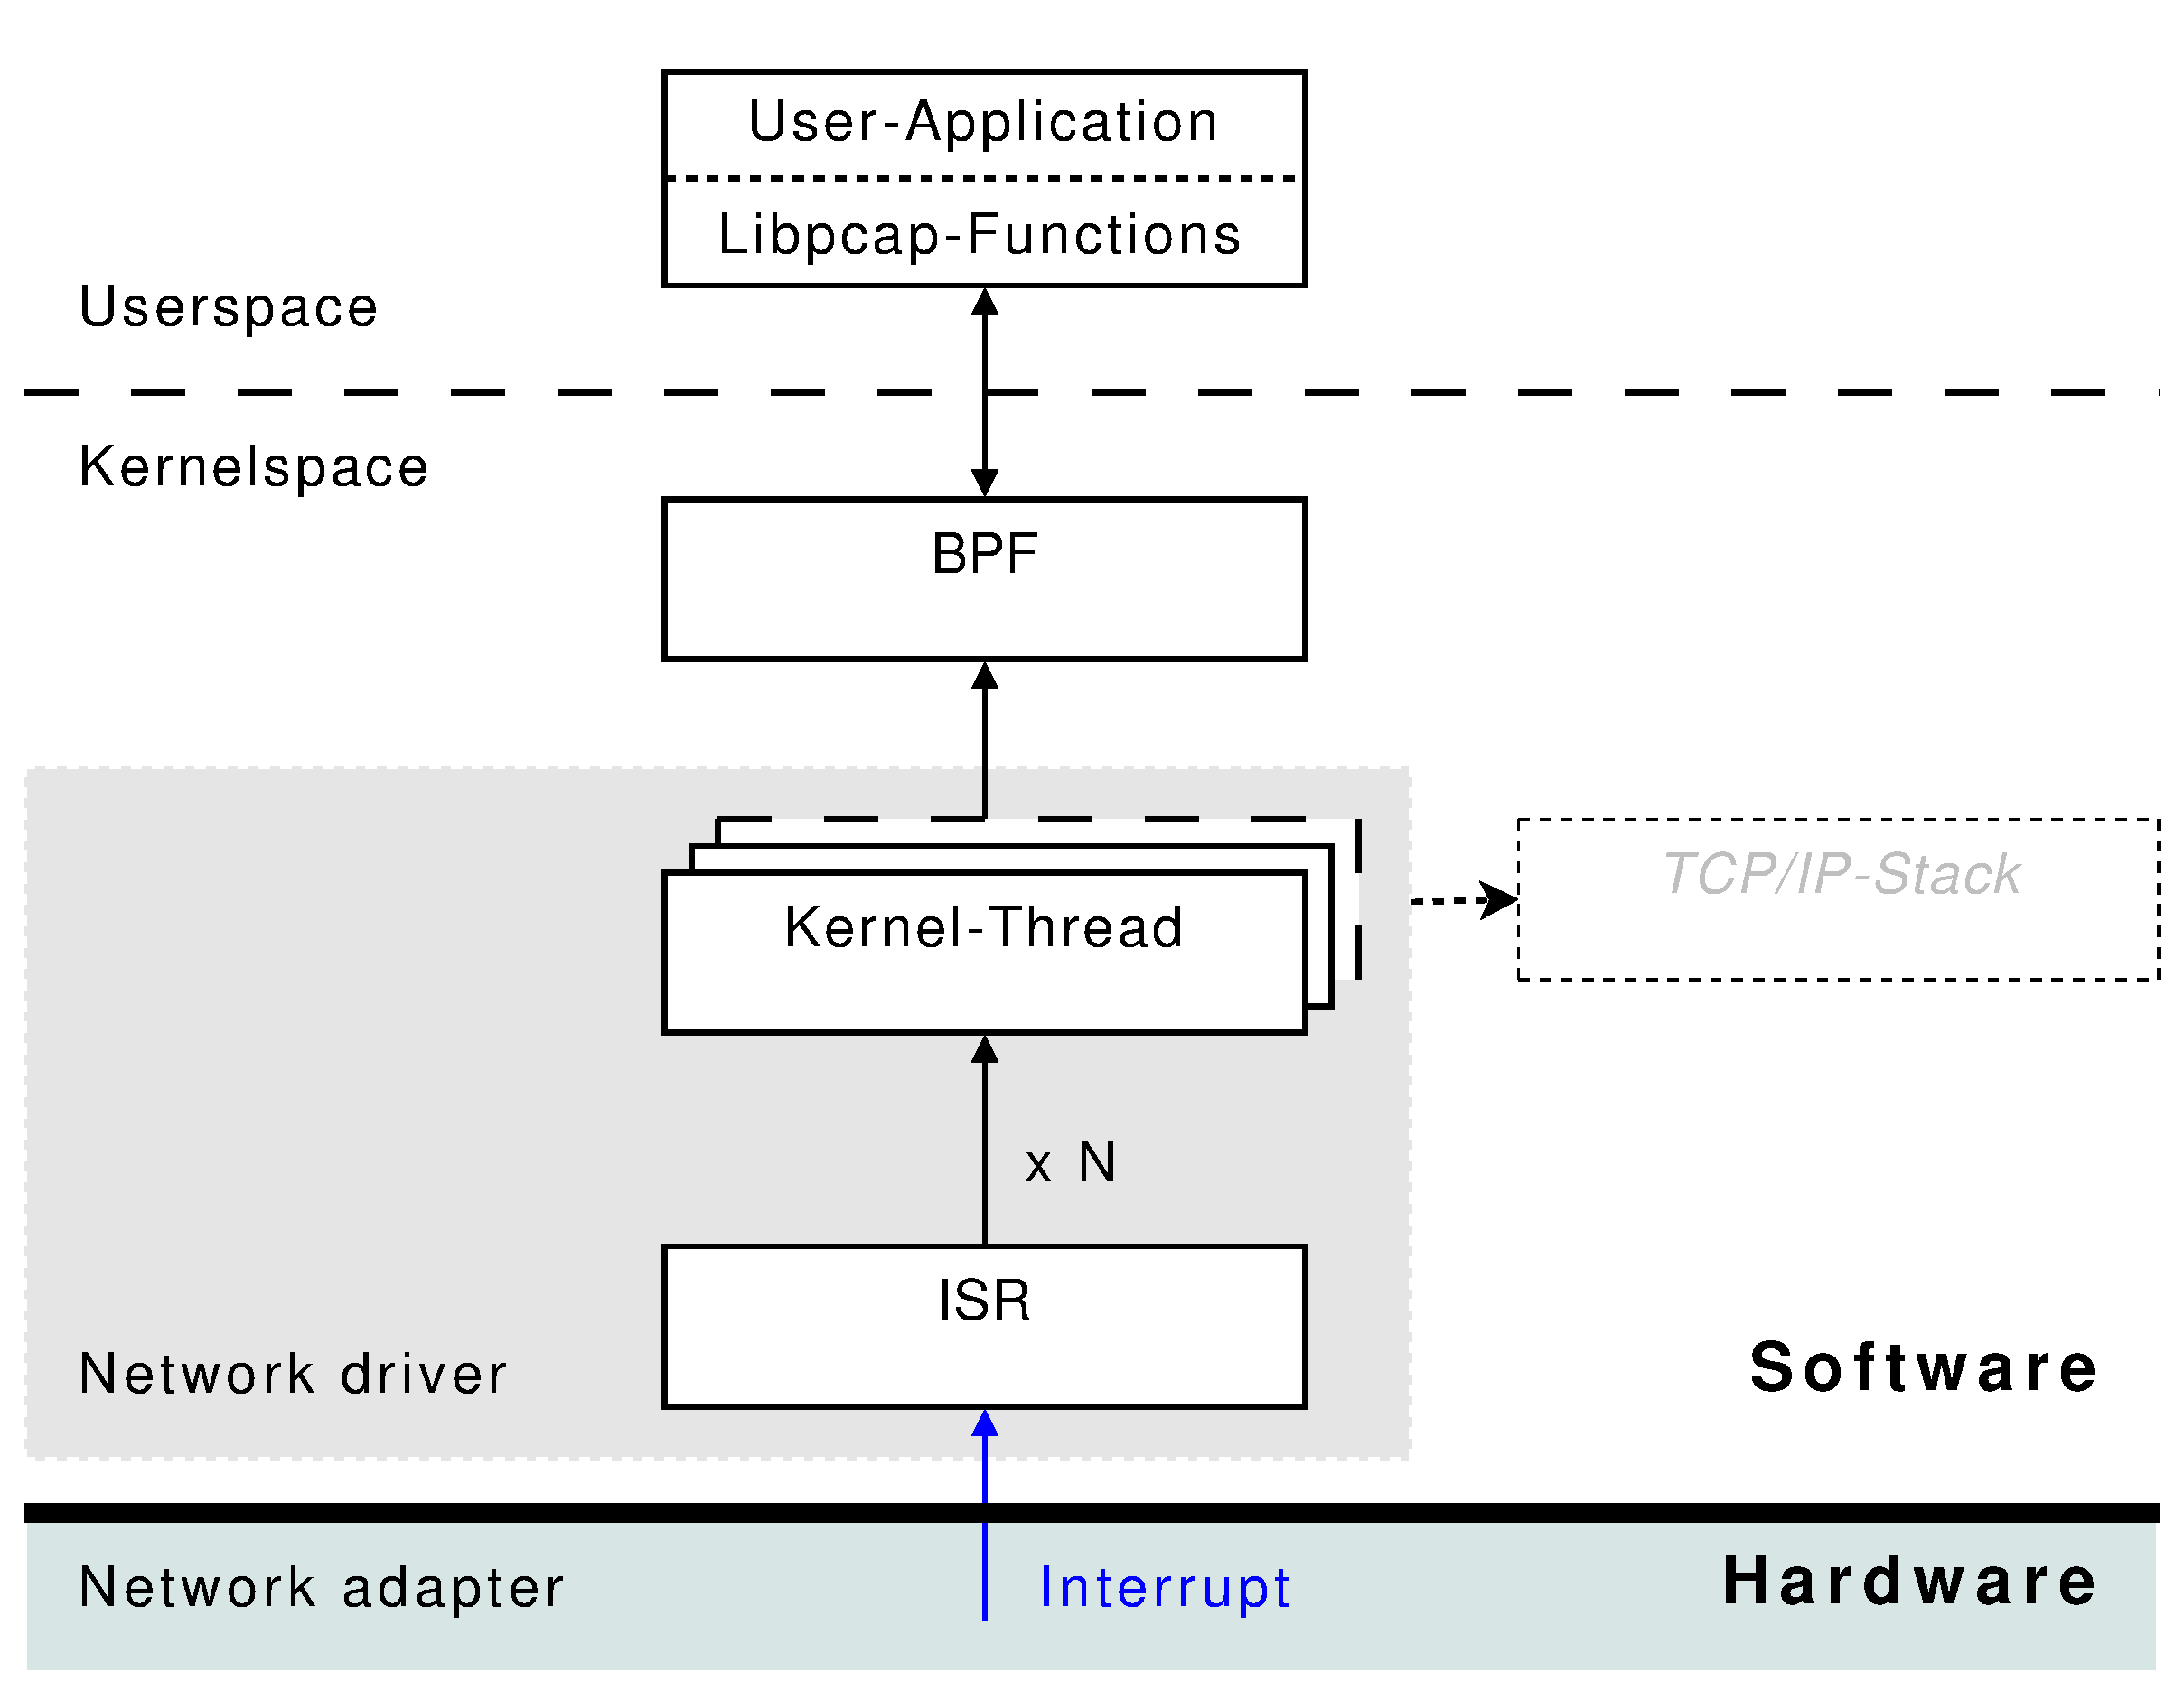
\includegraphics [height=65mm,width=60mm]{pics/PCS_funcs_ziel_DA_0}}
\only<2>{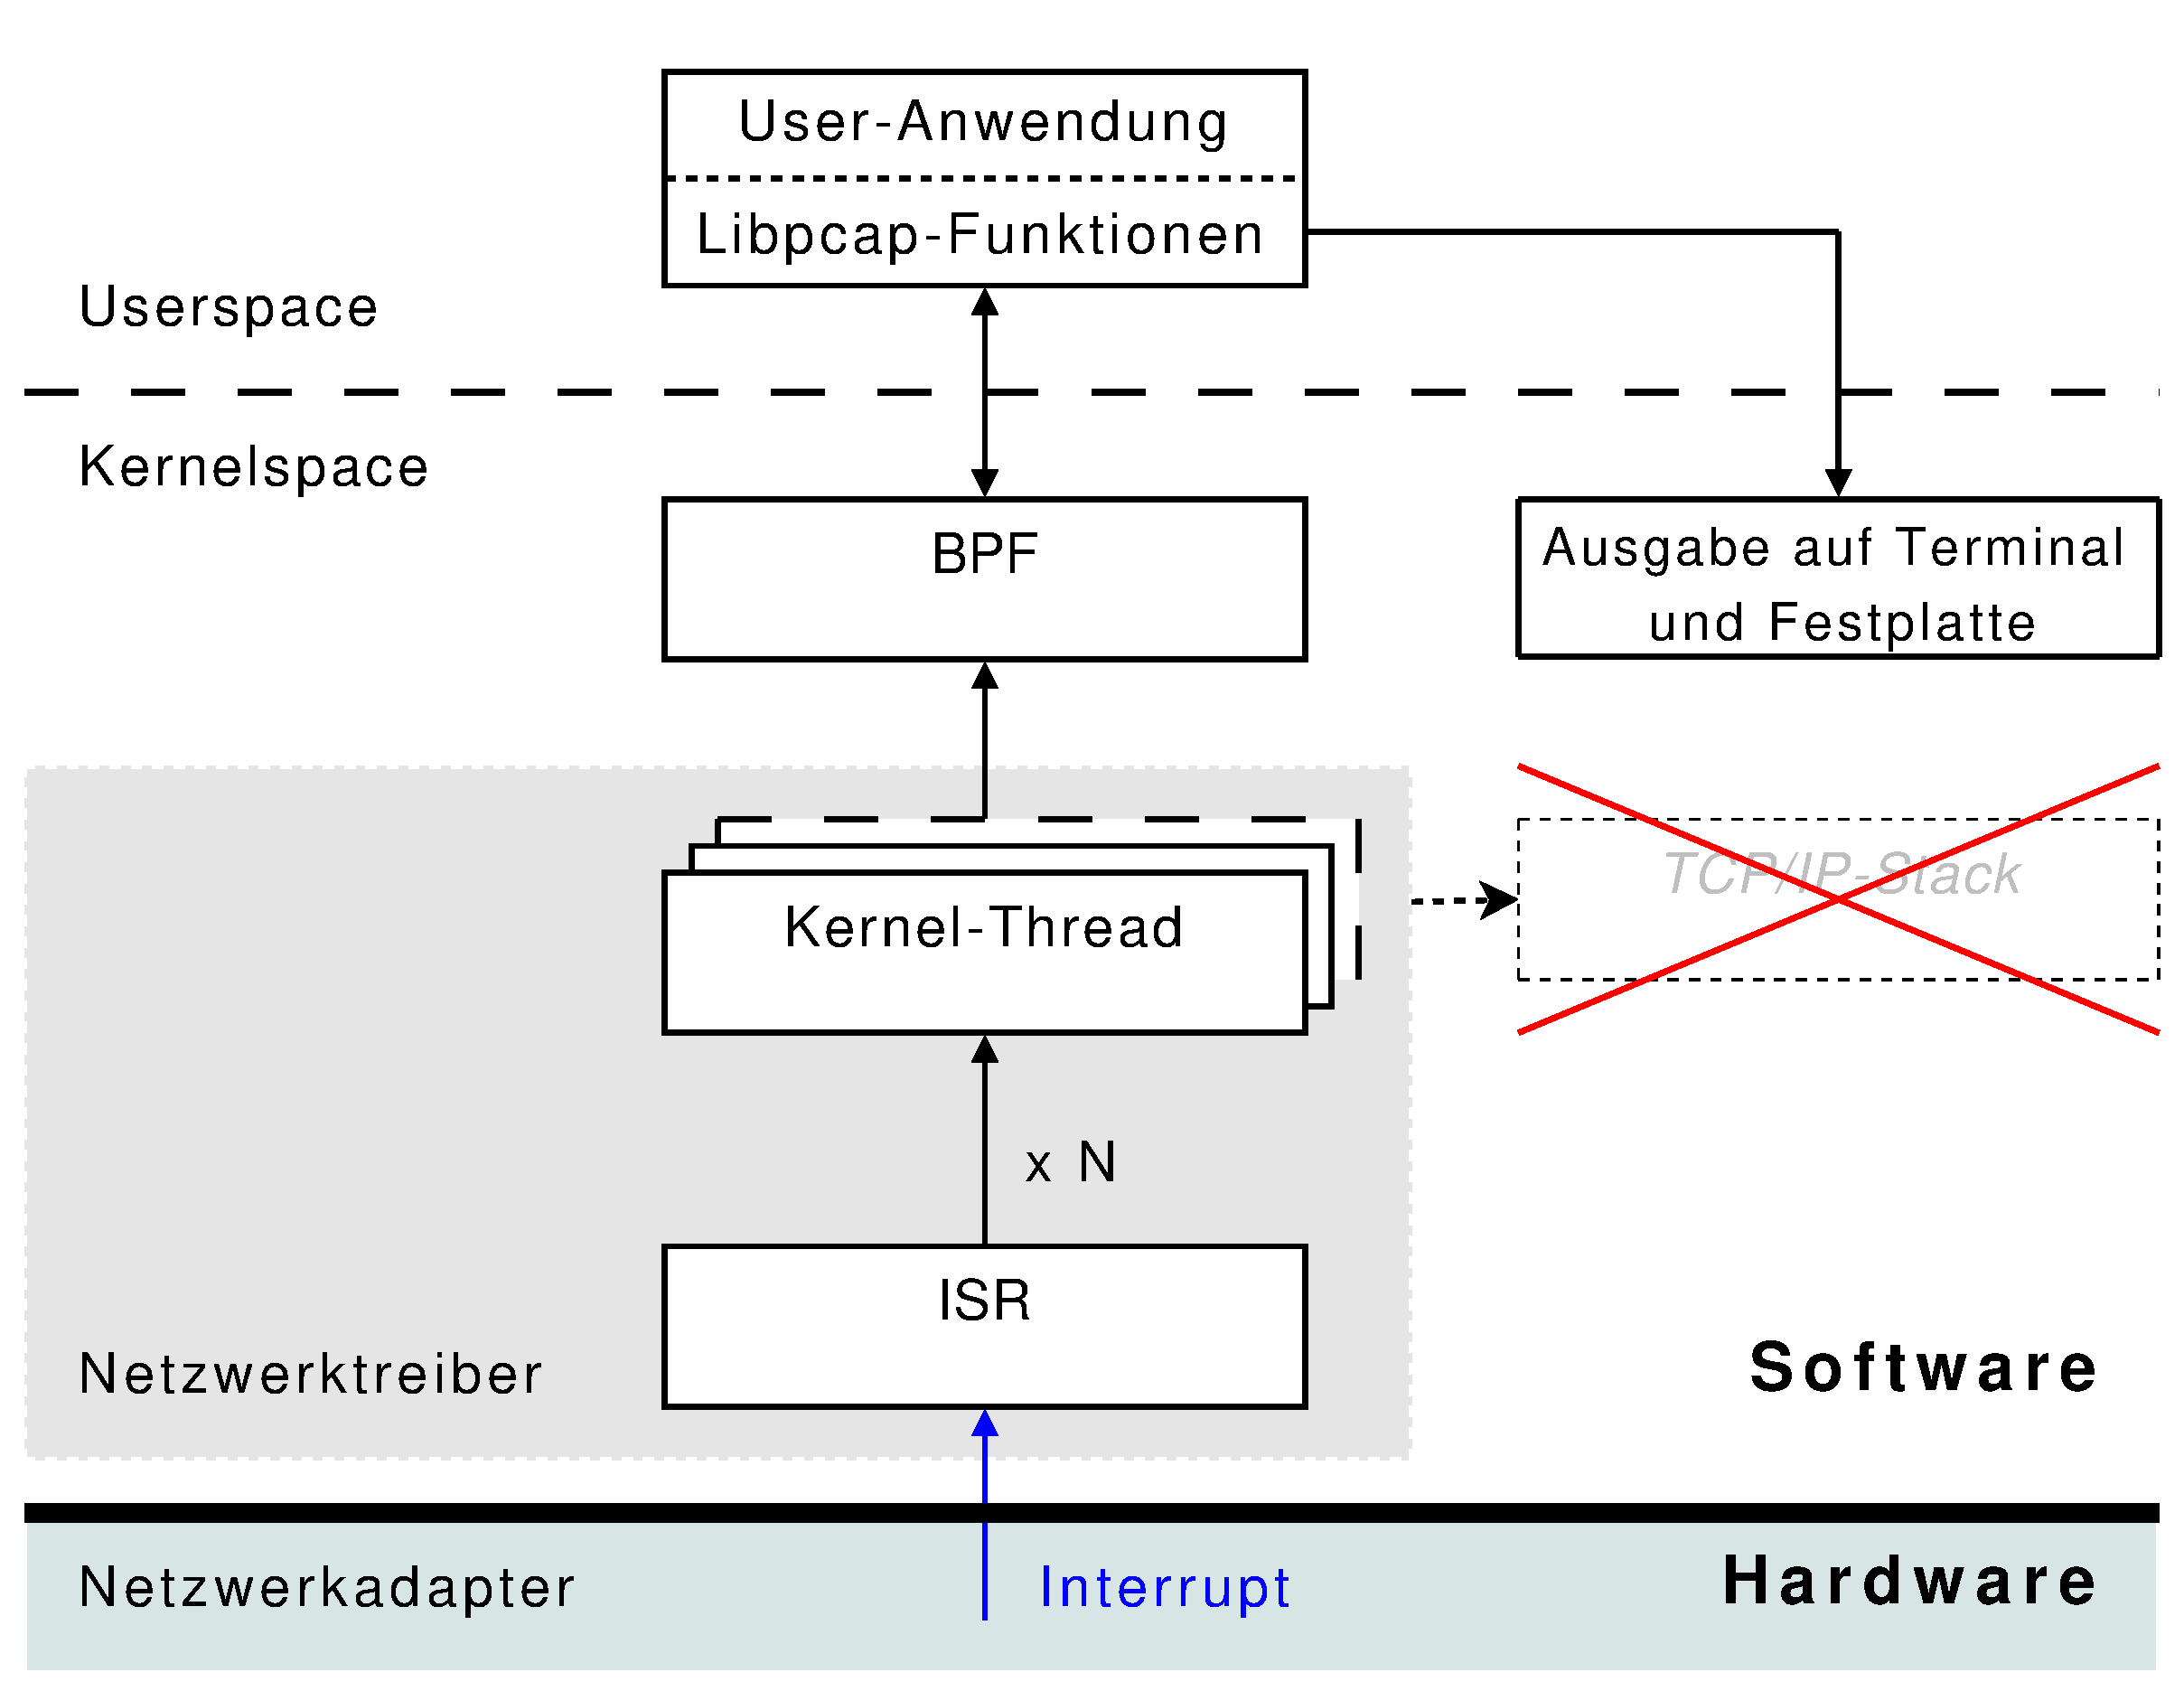
\includegraphics [height=65mm,width=60mm]{pics/PCS_funcs_ziel_DA_1}}
\only<3>{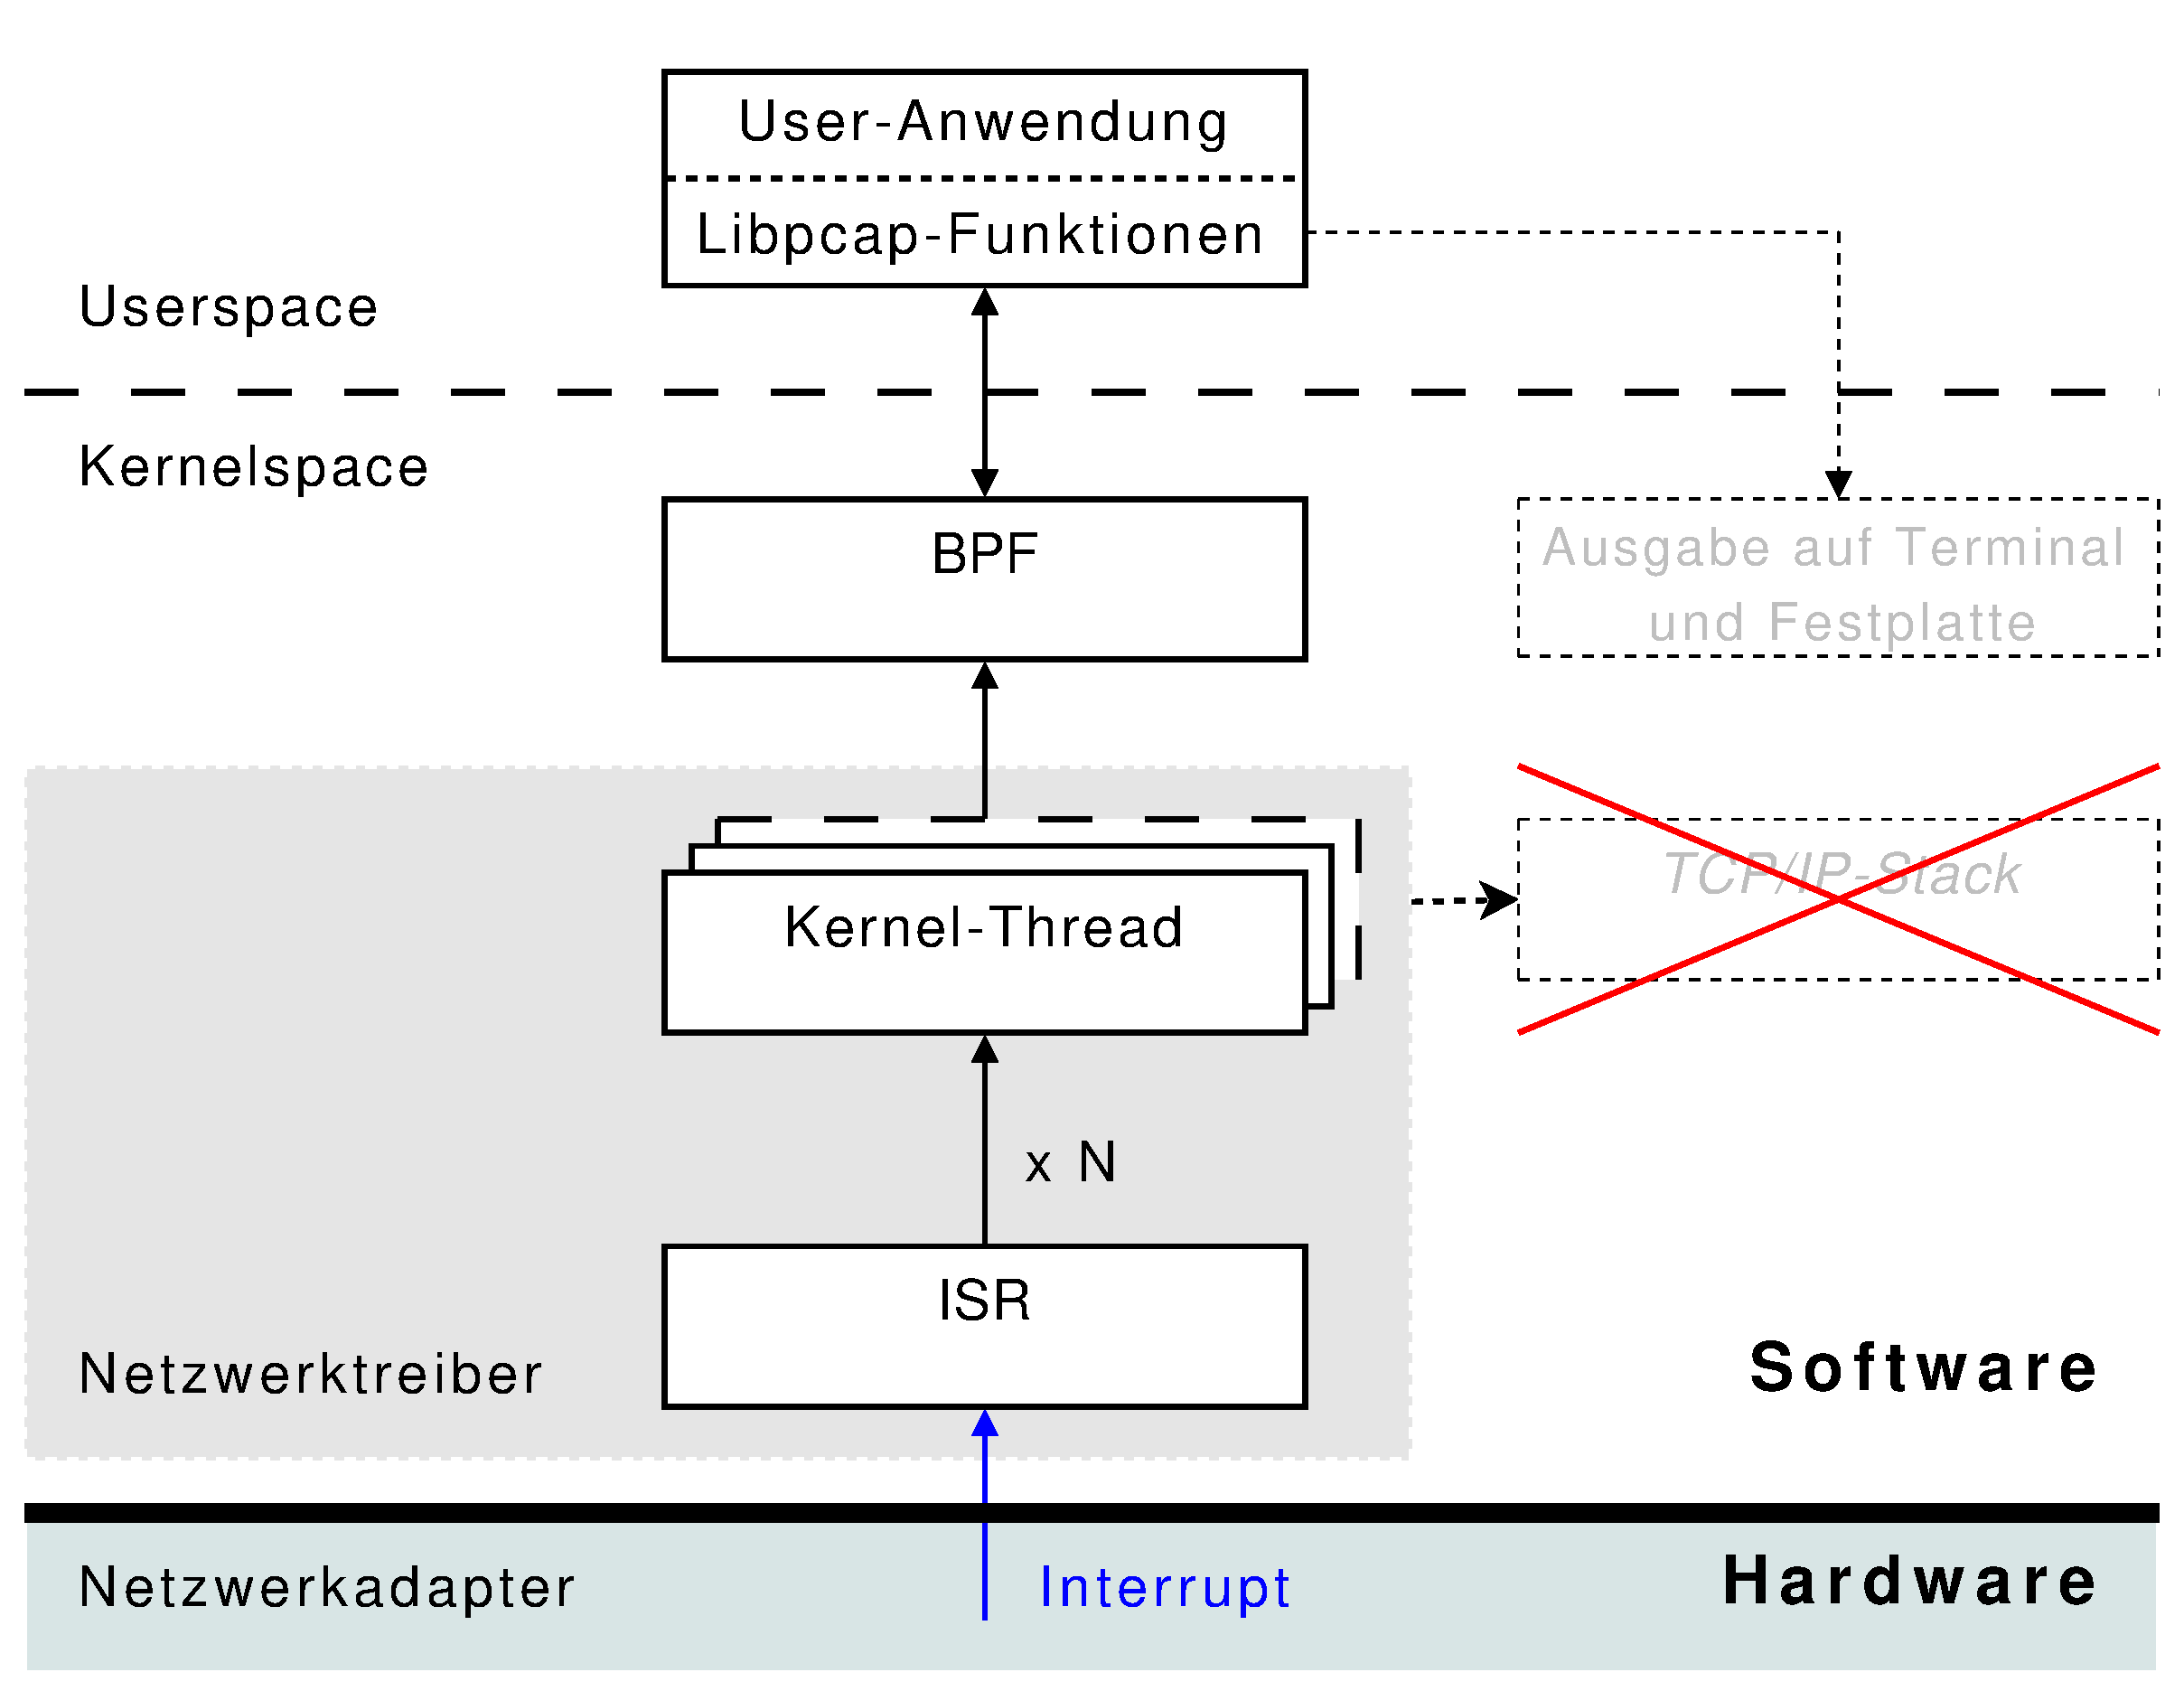
\includegraphics [height=65mm,width=60mm]{pics/PCS_funcs_ziel_DA_2}}
\only<4>{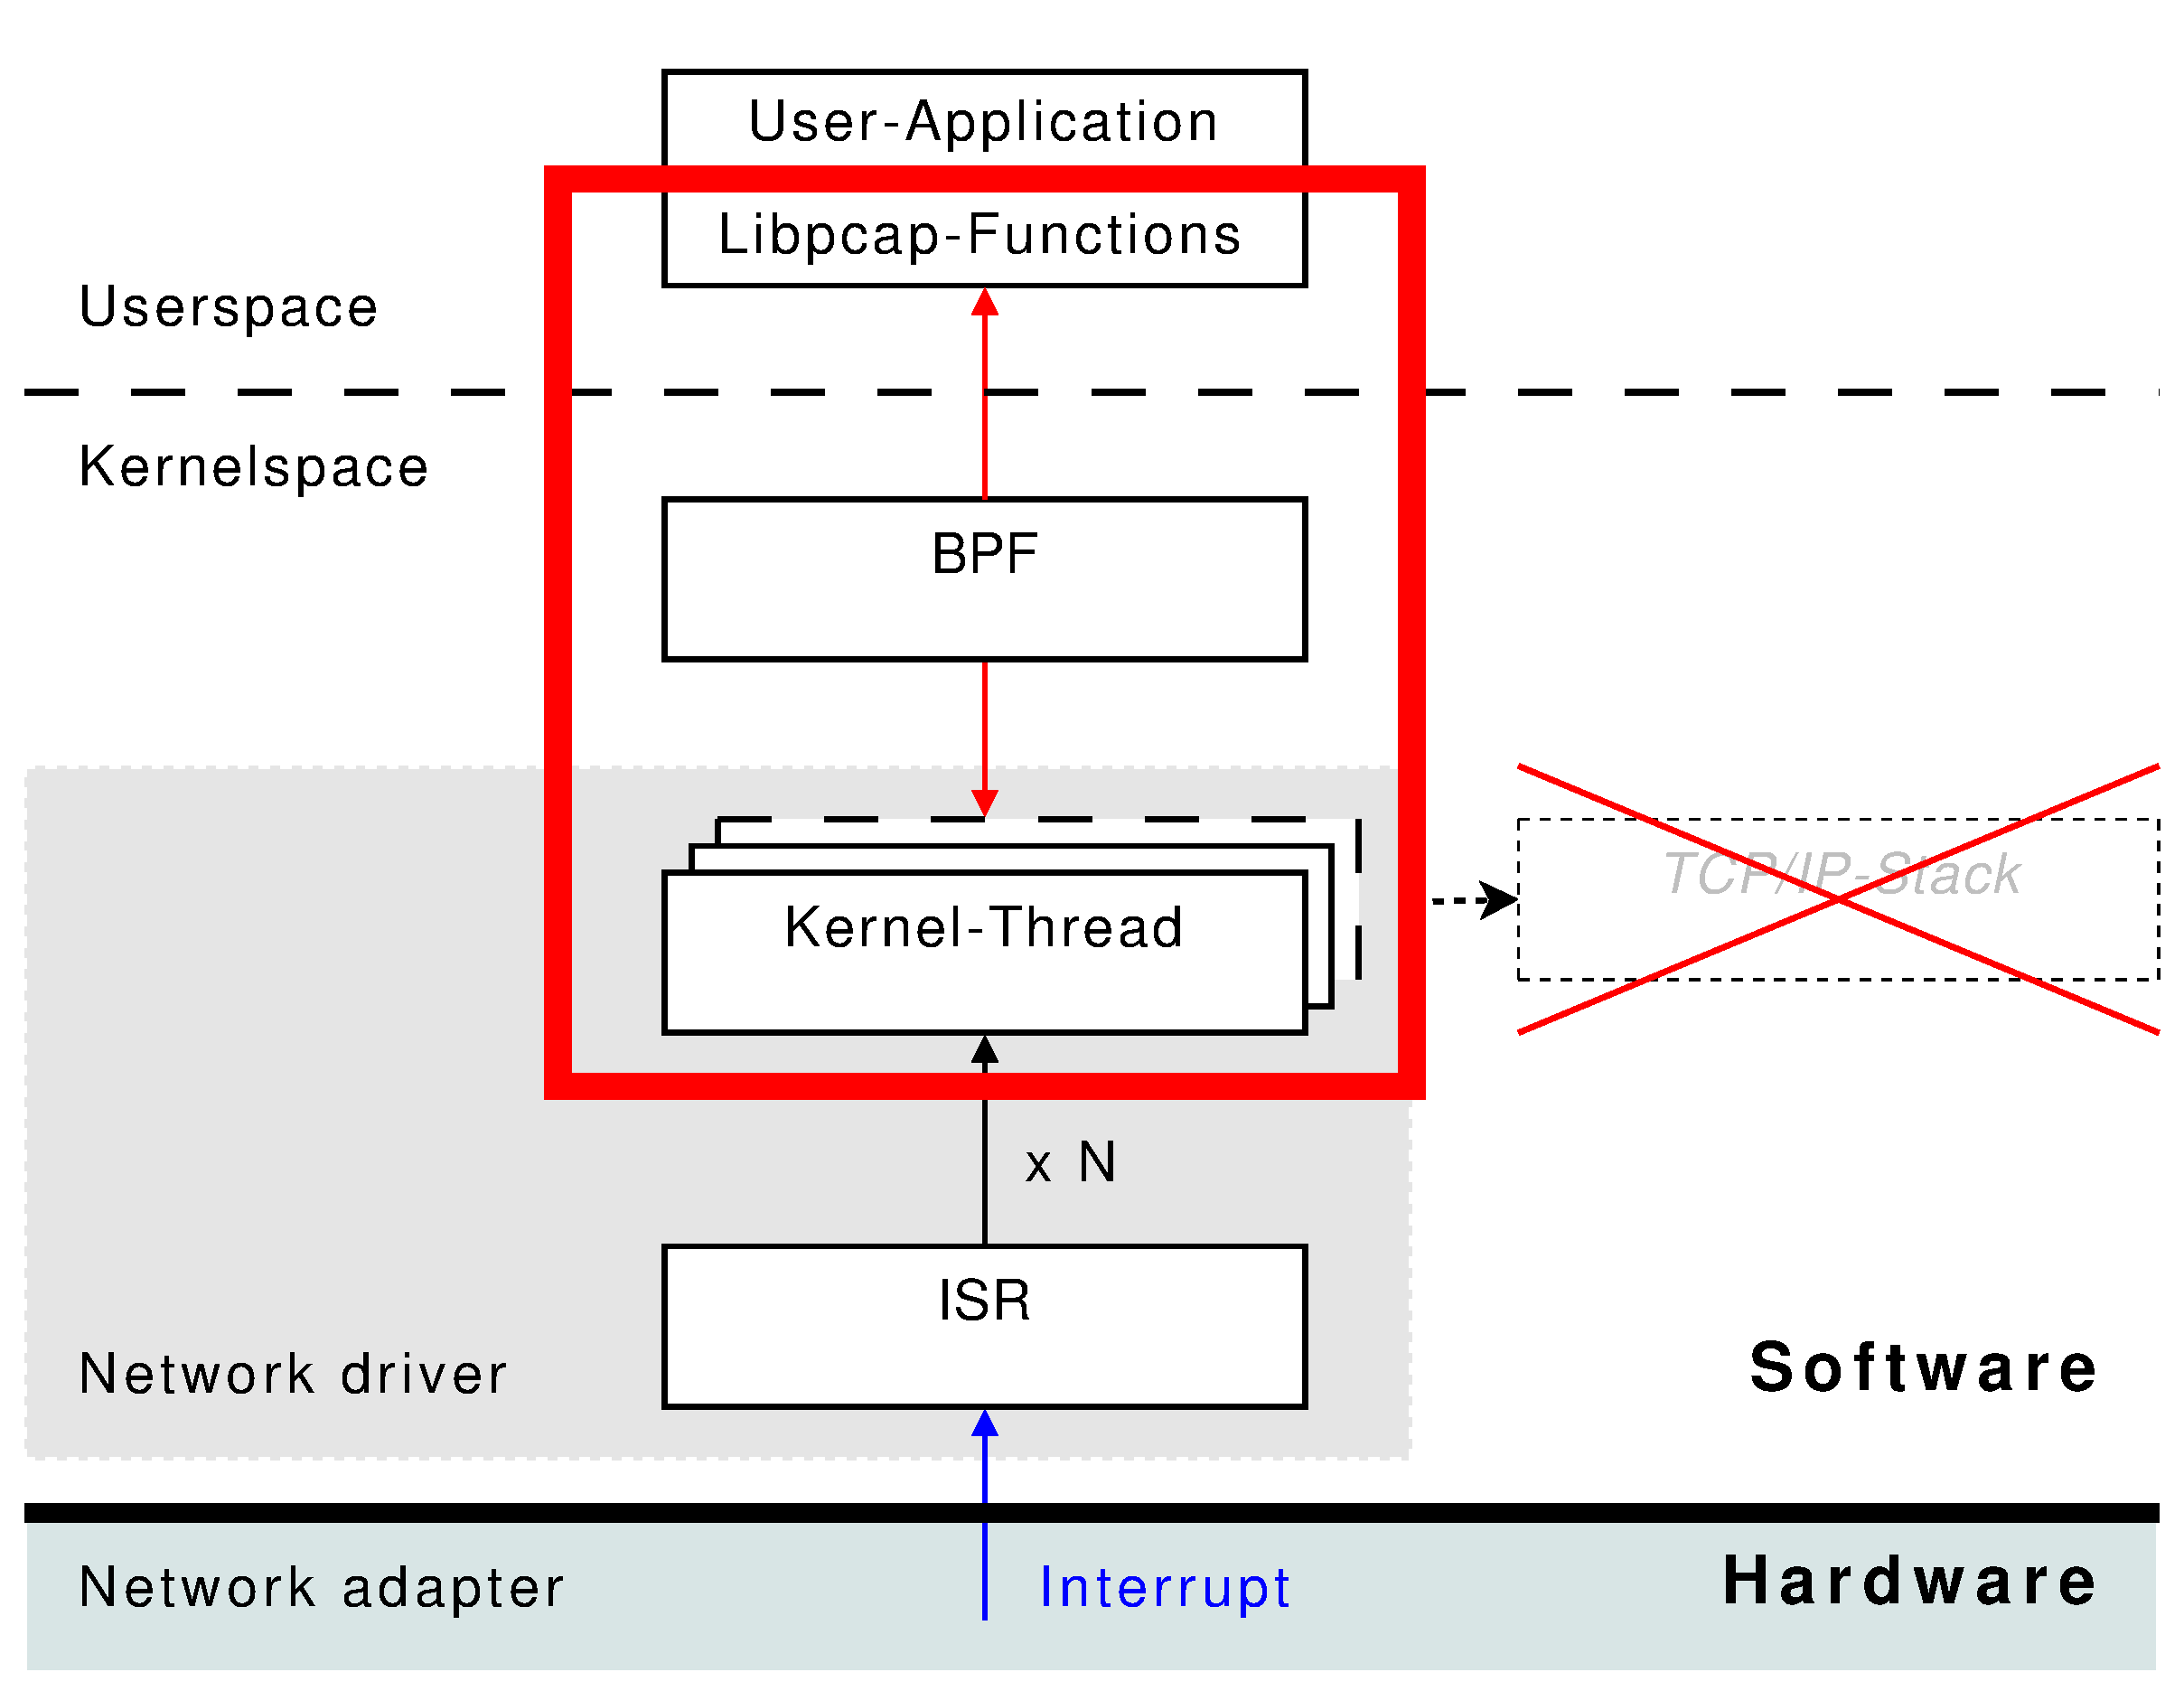
\includegraphics [height=65mm,width=60mm]{pics/PCS_funcs_ziel_DA}}
\end{columns}
\end{frame}

\subsection*{Vom generic zum ringmap}
%%%%%%%%%%%%%%%%%%%%%%%%%%%%%%%%%%%%%%%%%%%%%%%%%%%%%%%%%%%%%%%%%%%

\begin{frame}
\frametitle{Vom generic zum ringmap}
\begin{columns}
\column[t]{0.5\textwidth}
\vspace{-1em}
\begin{itemize}
	\item<2->Eliminieren Kopie-Vorg"ange und Systemaufrufe
	\item<3->BPF-Puffer wird nicht mehr gebraucht
	\item<4->Paket-Puffer in den Userspace einblenden
	\item<5->BPF in den Userspace verschieben
	\item<6->\textbf{ringmap}-Packet-Capturing-Stack
\end{itemize}
\column[t]{0.5\textwidth}
\vspace{-2em}
\only<1>{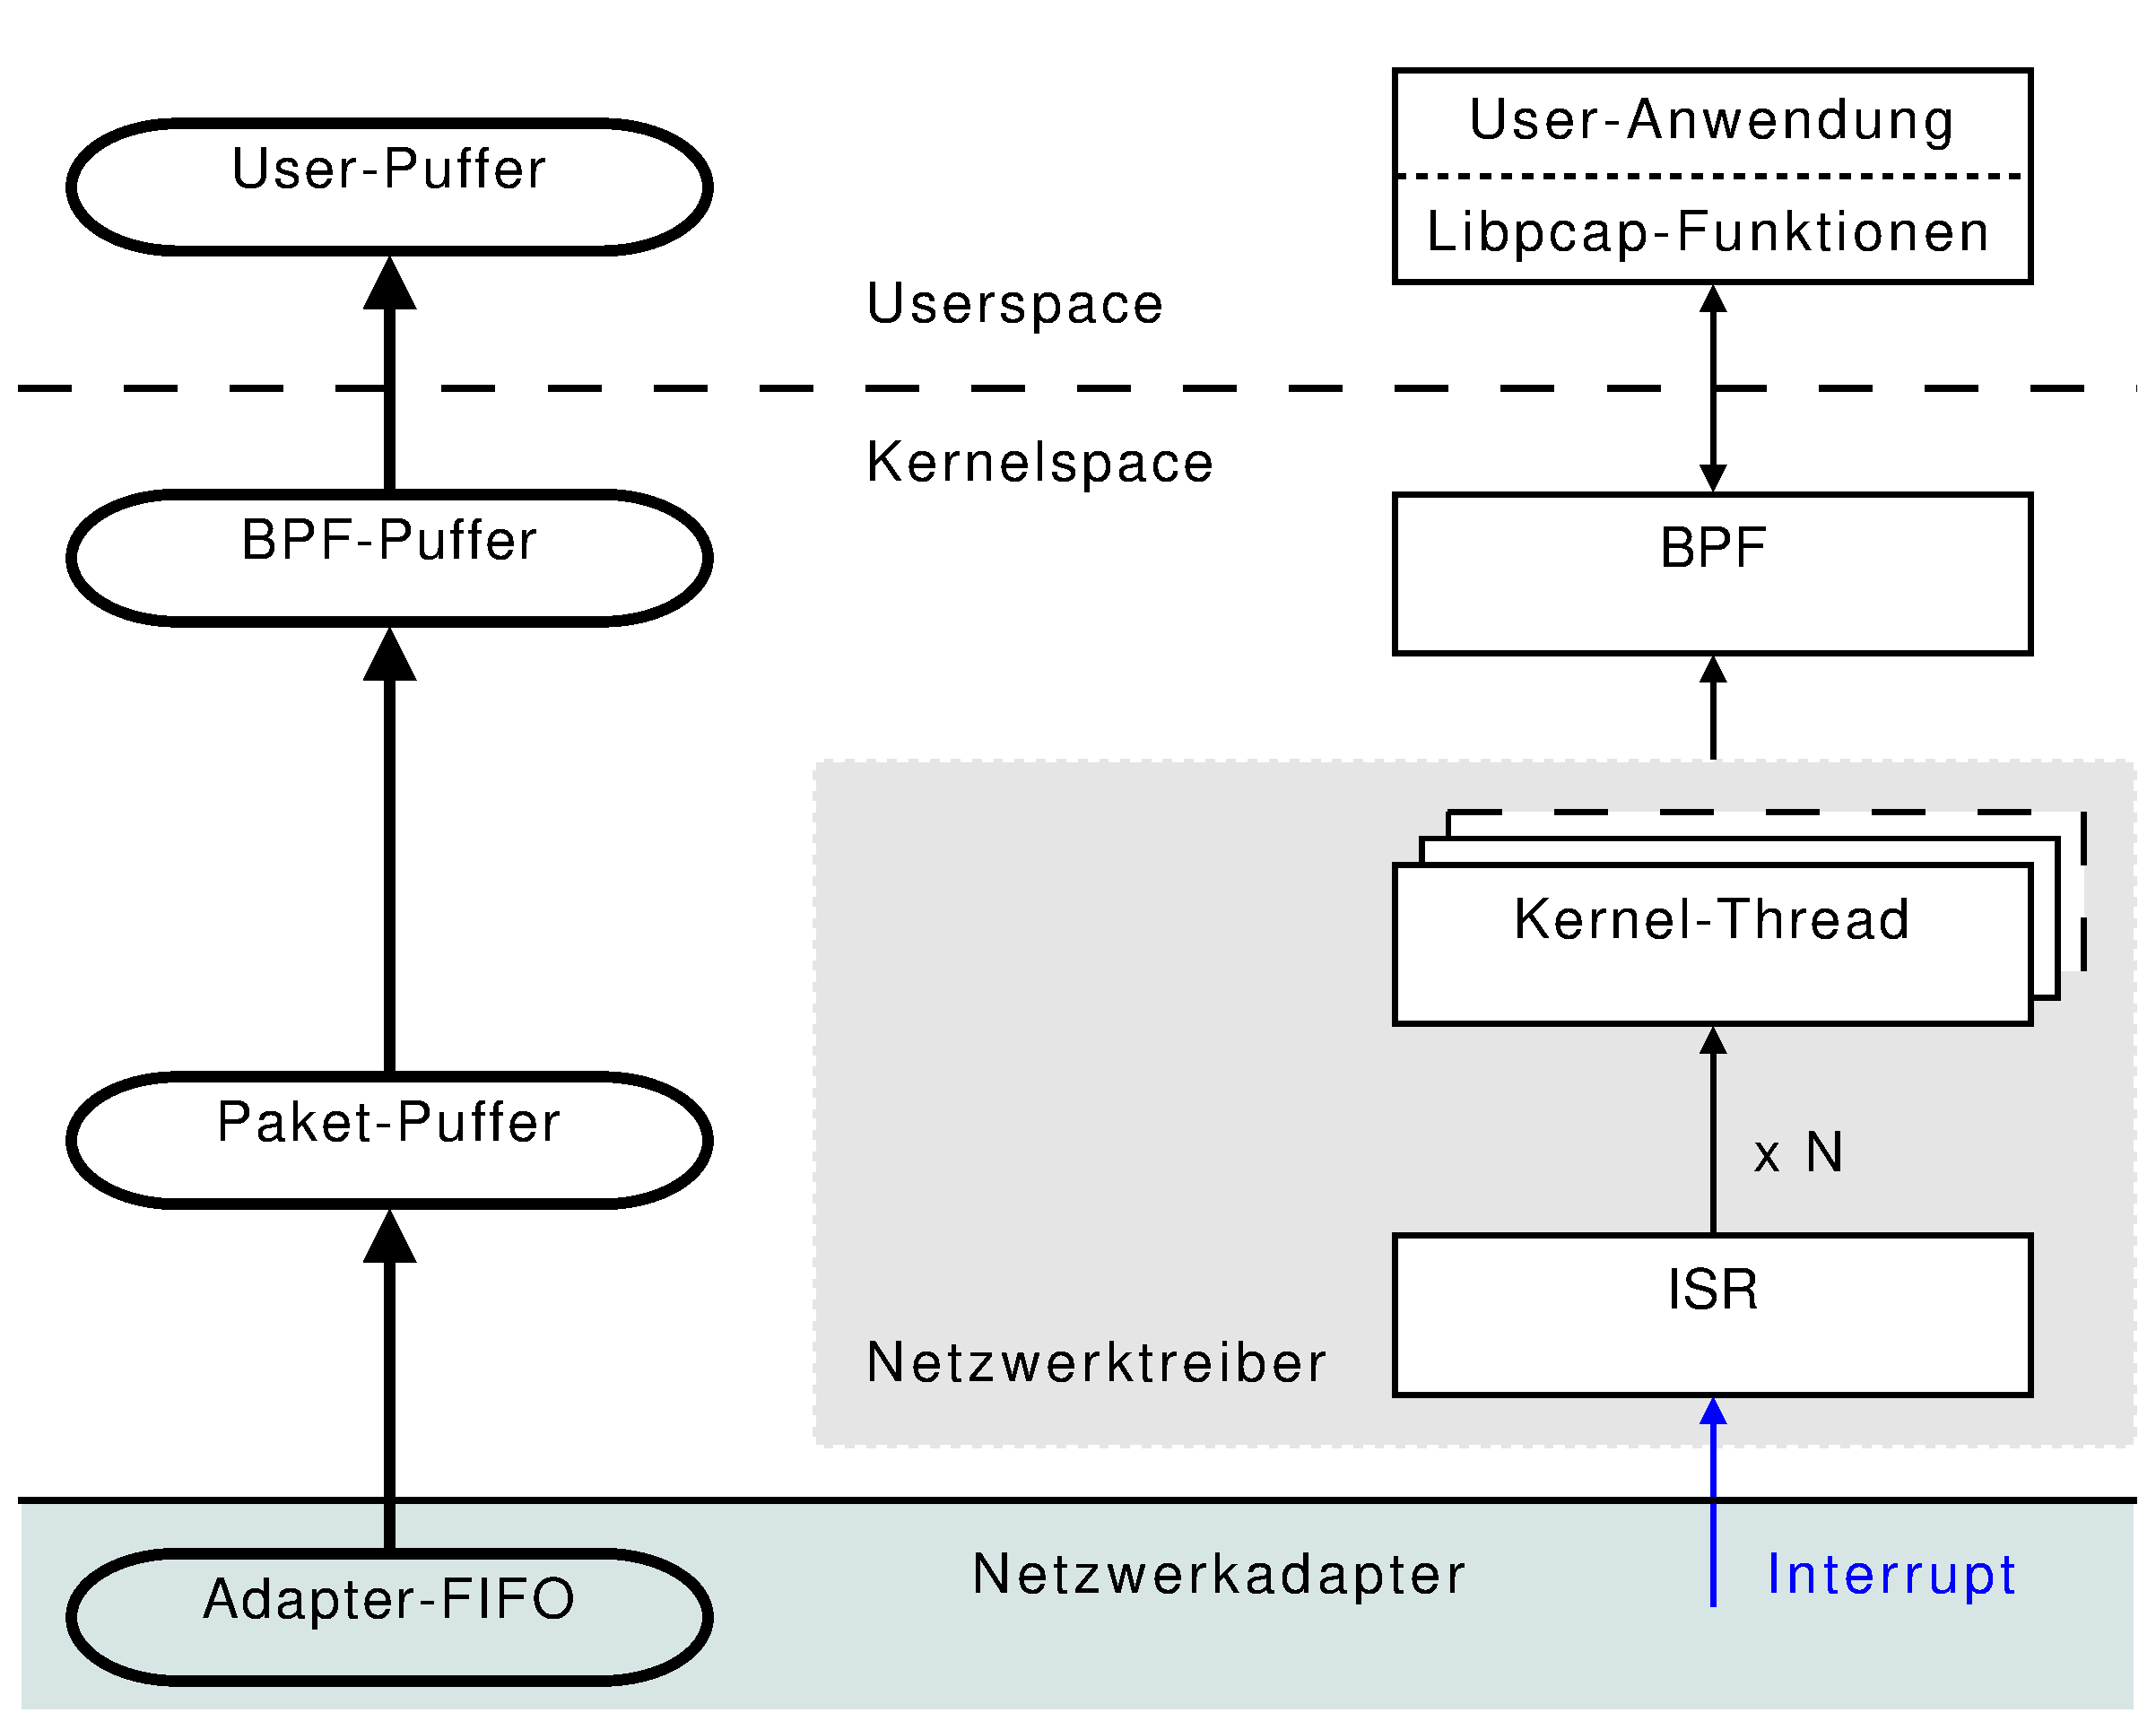
\includegraphics [height=59mm,width=60mm]{pics/3copy}}
\only<2>{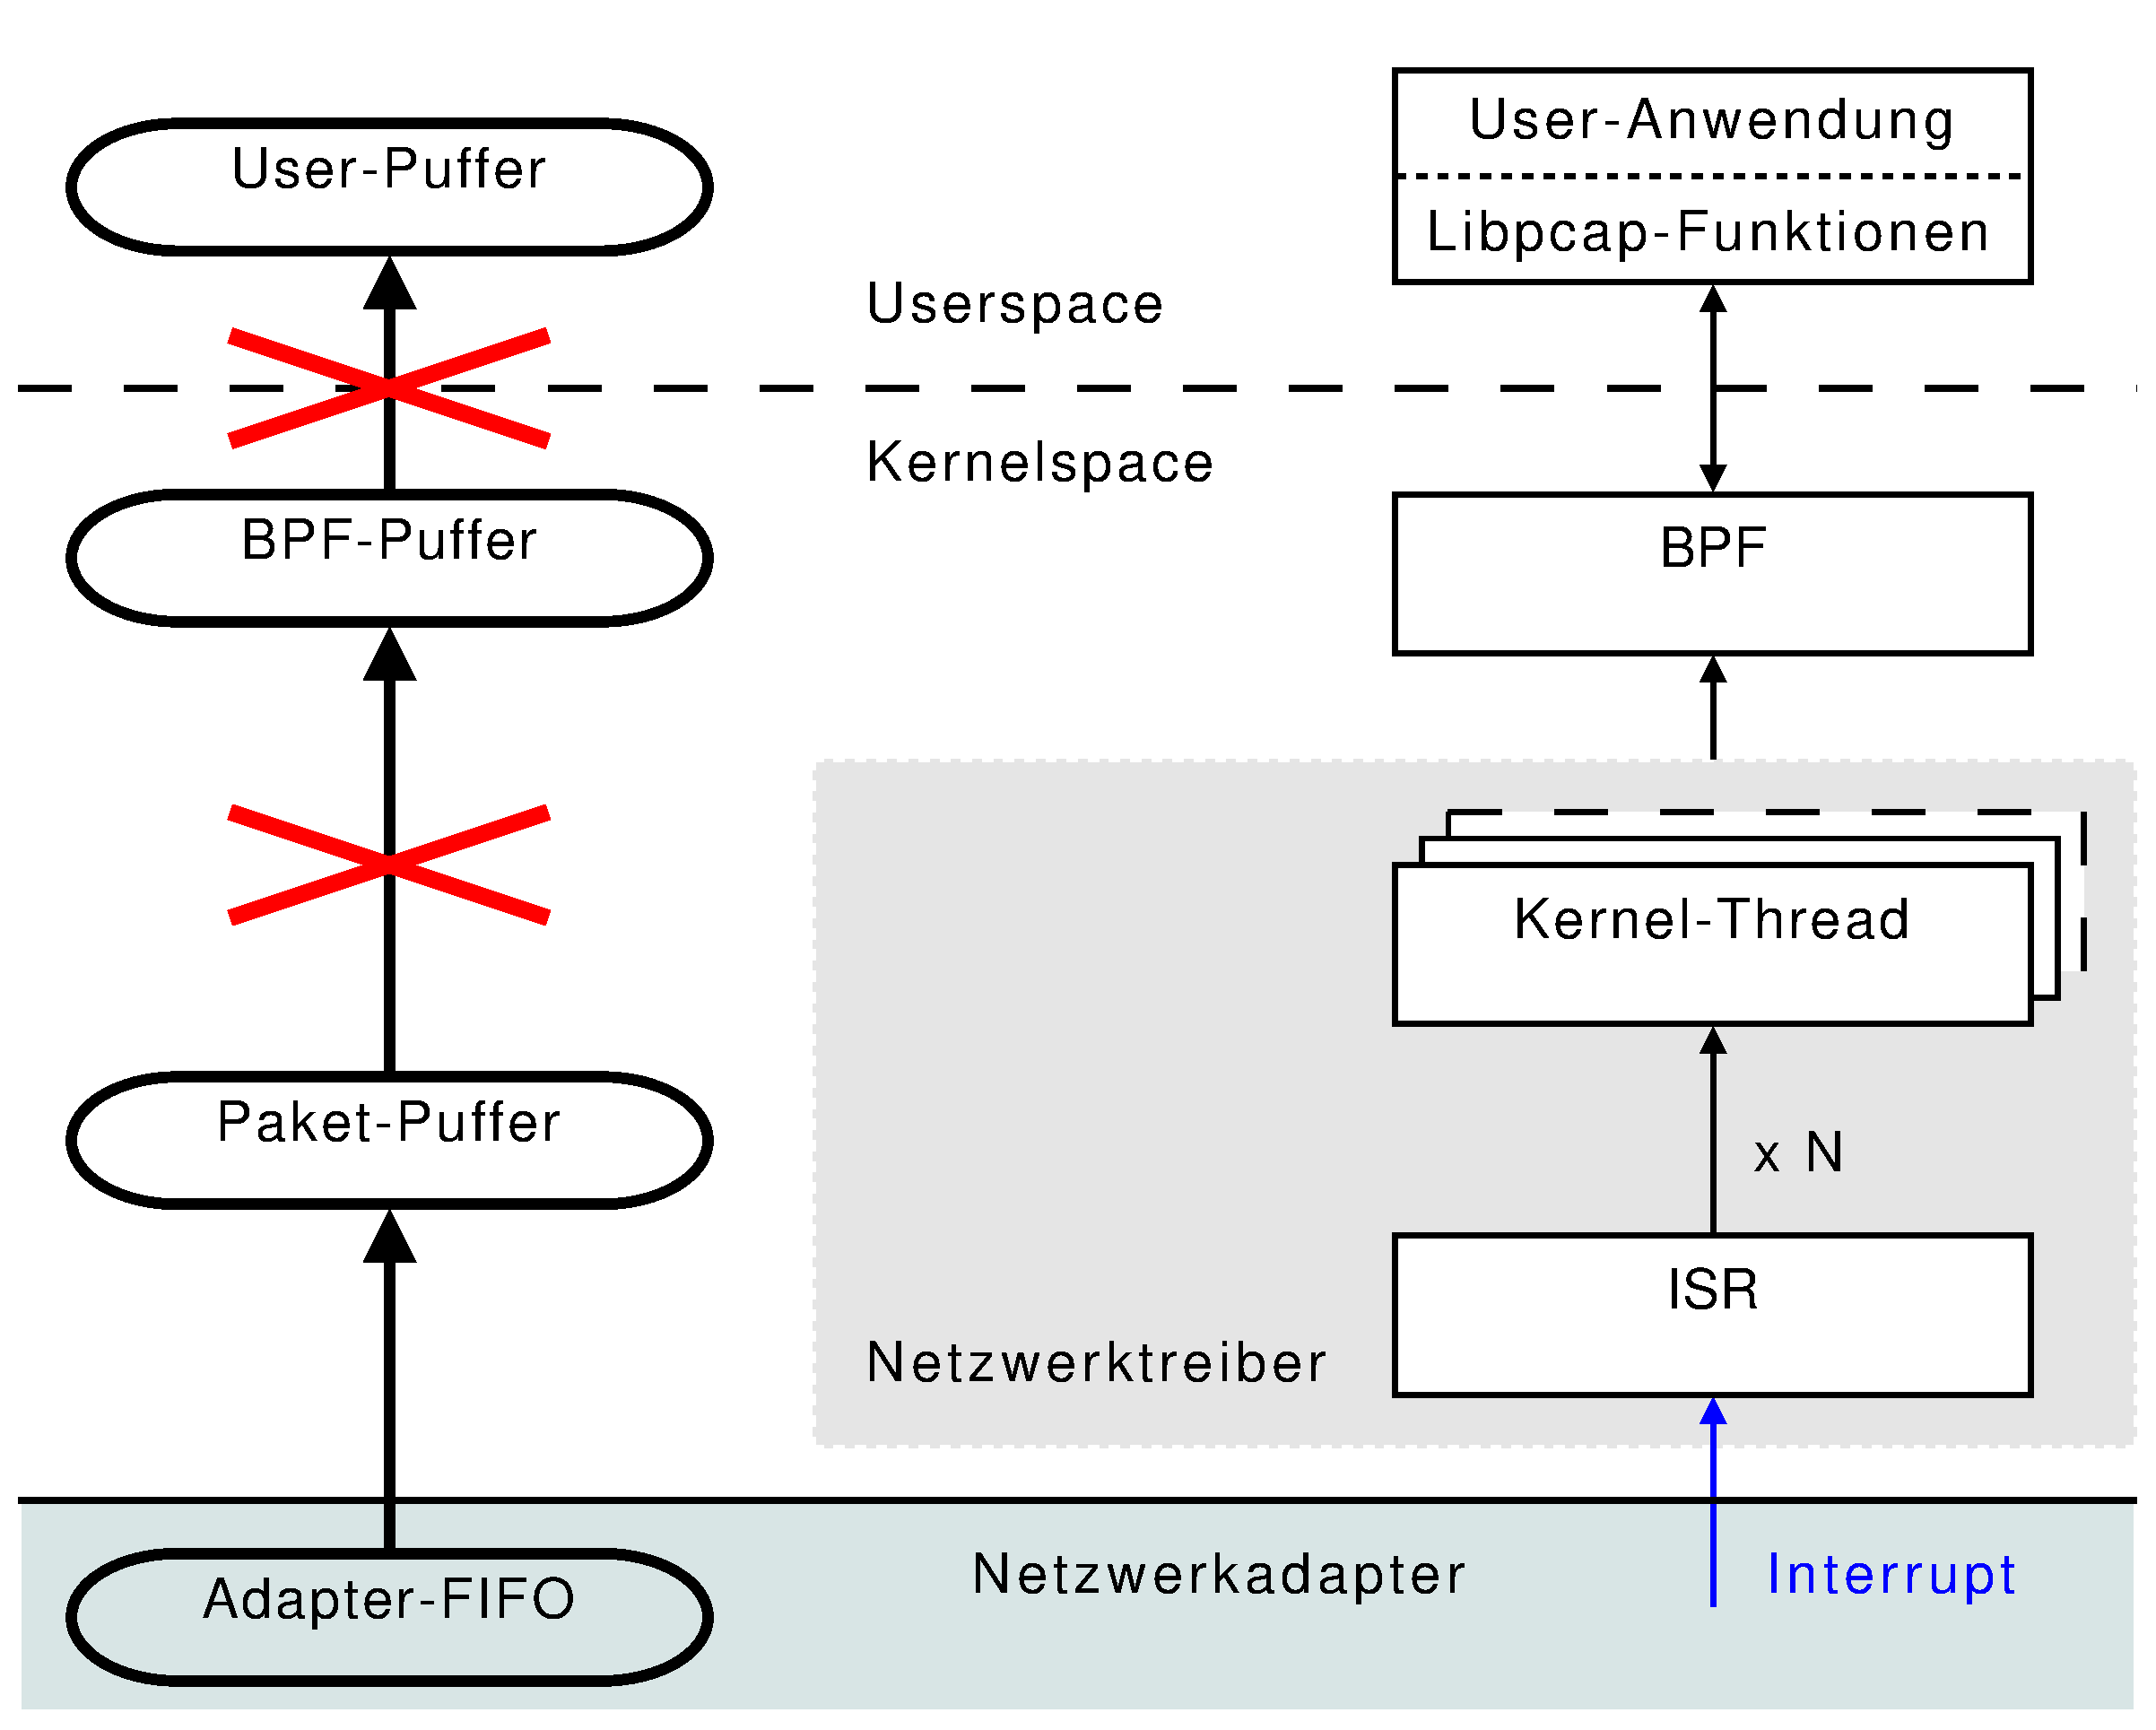
\includegraphics [height=59mm,width=60mm]{pics/3copy_solution_1}}
\only<3>{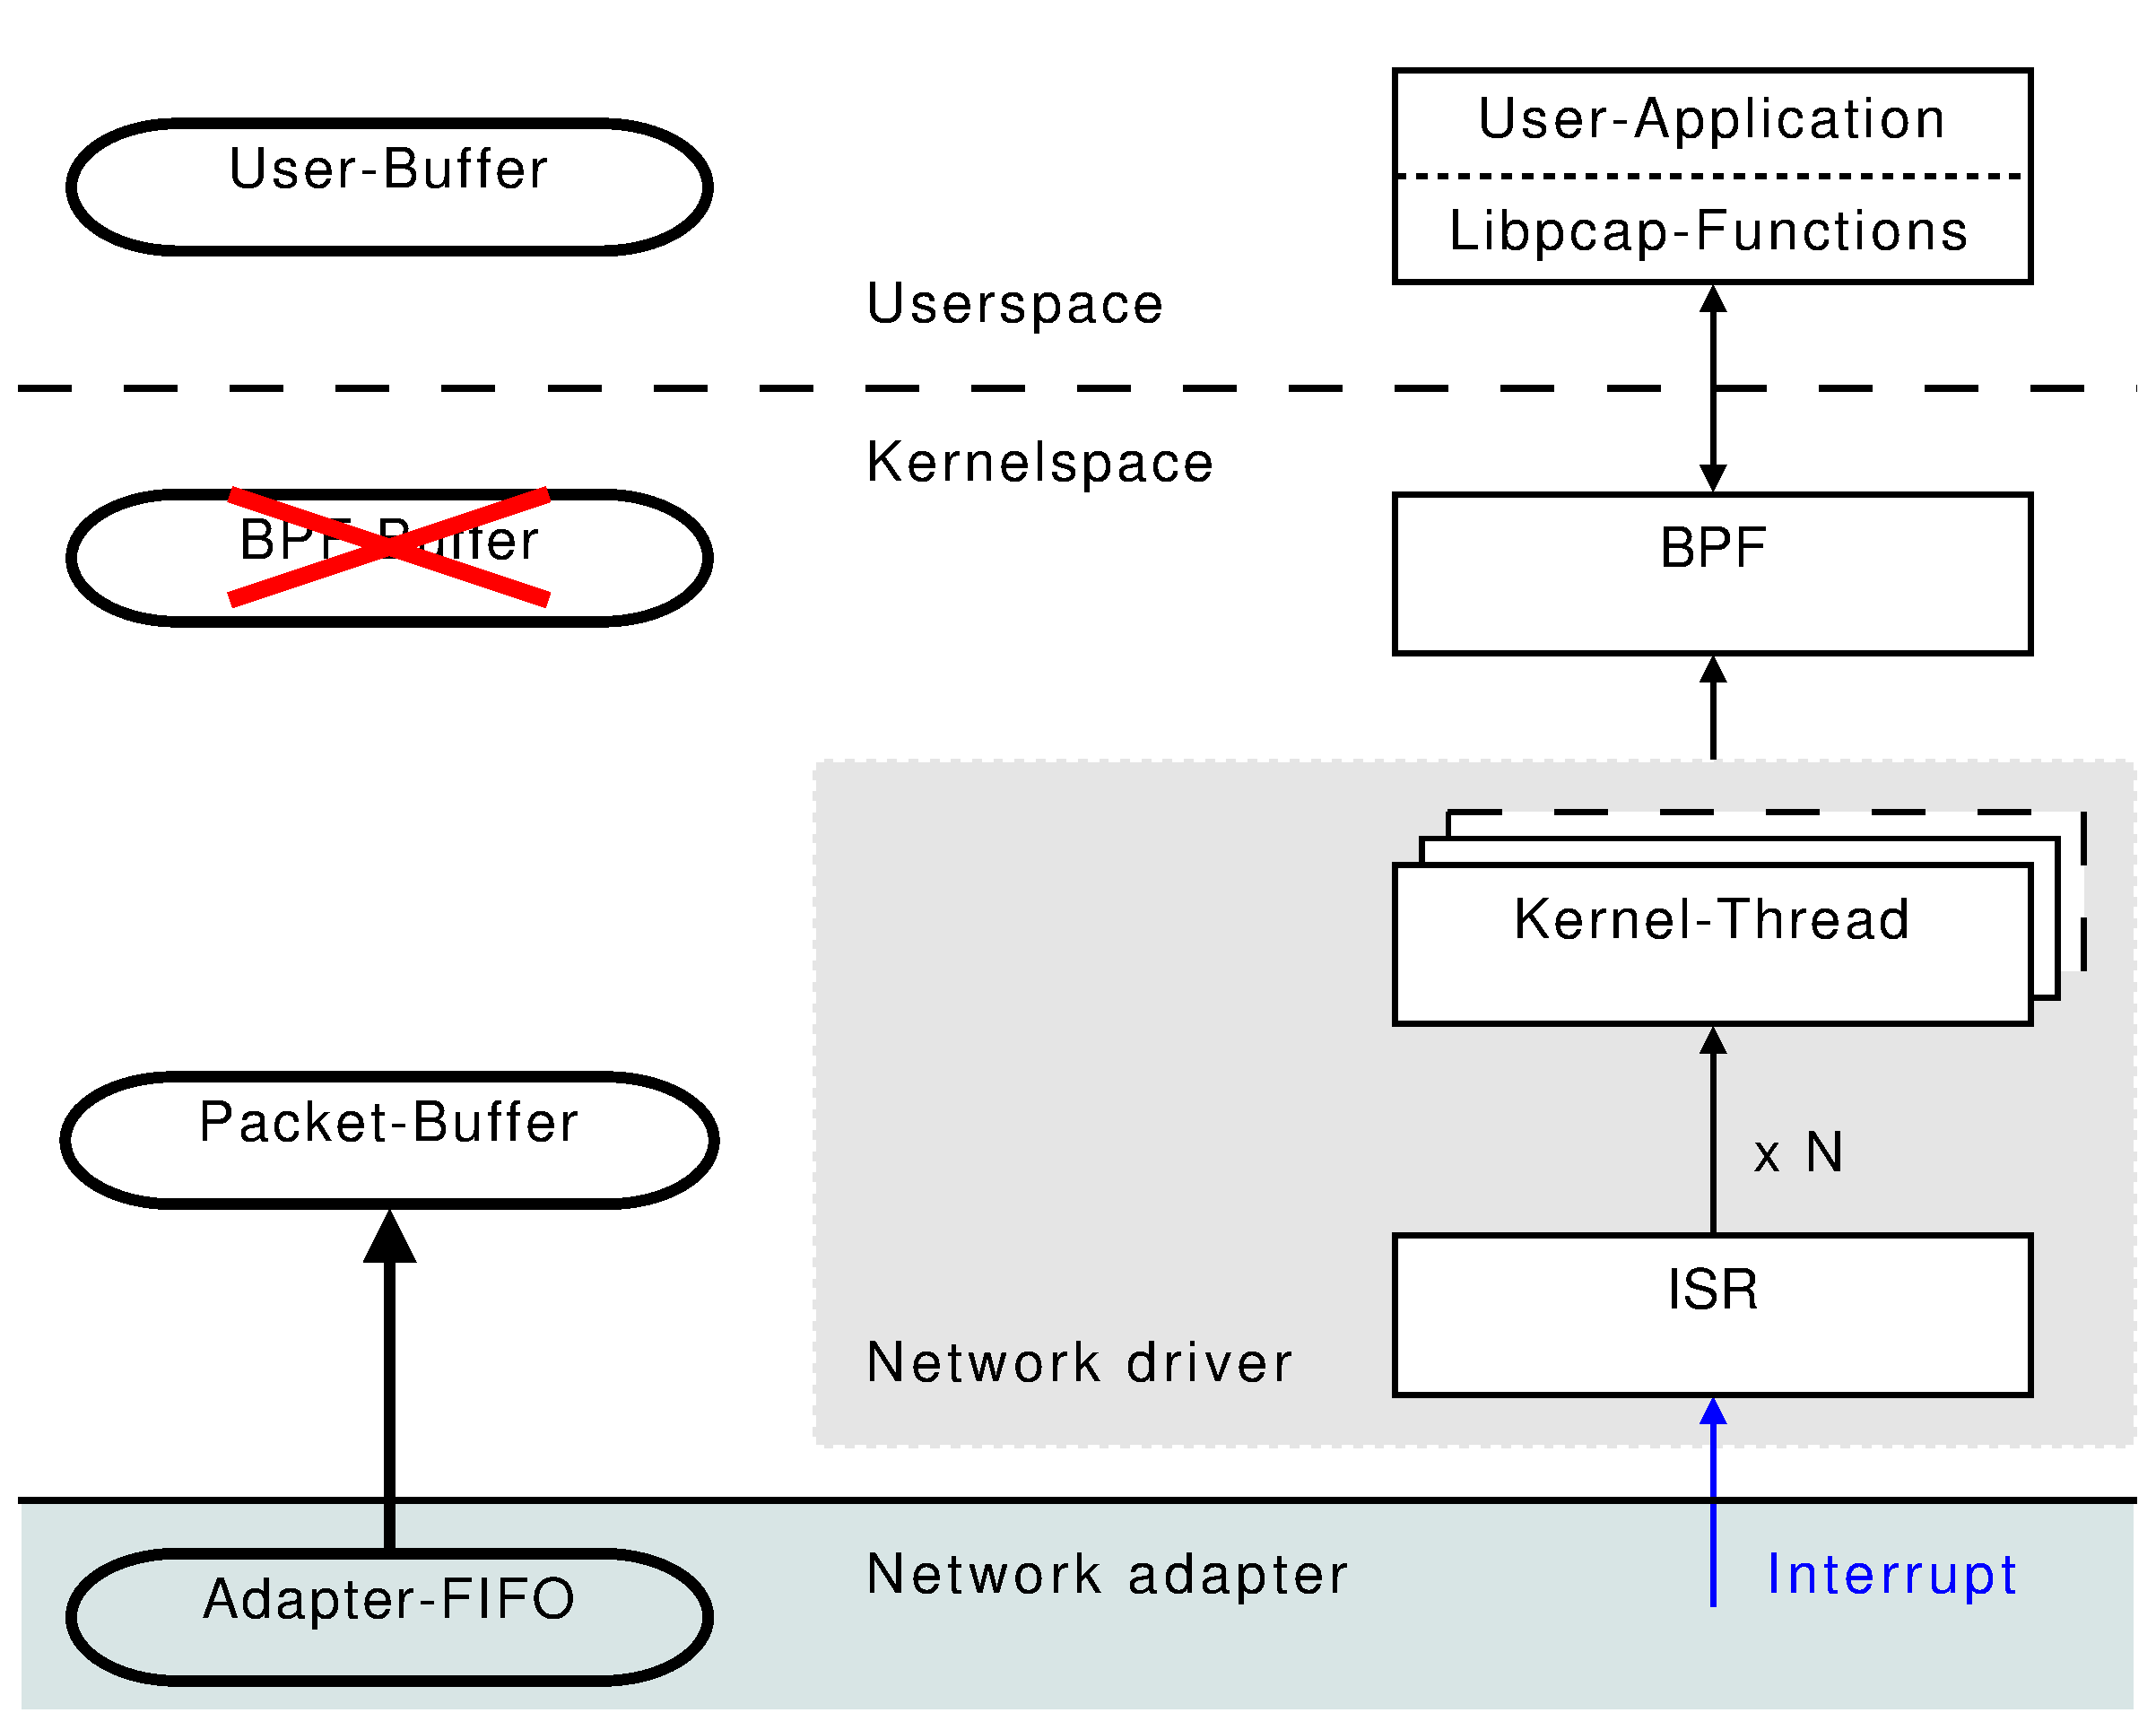
\includegraphics [height=59mm,width=60mm]{pics/3copy_solution_2}}
\only<4>{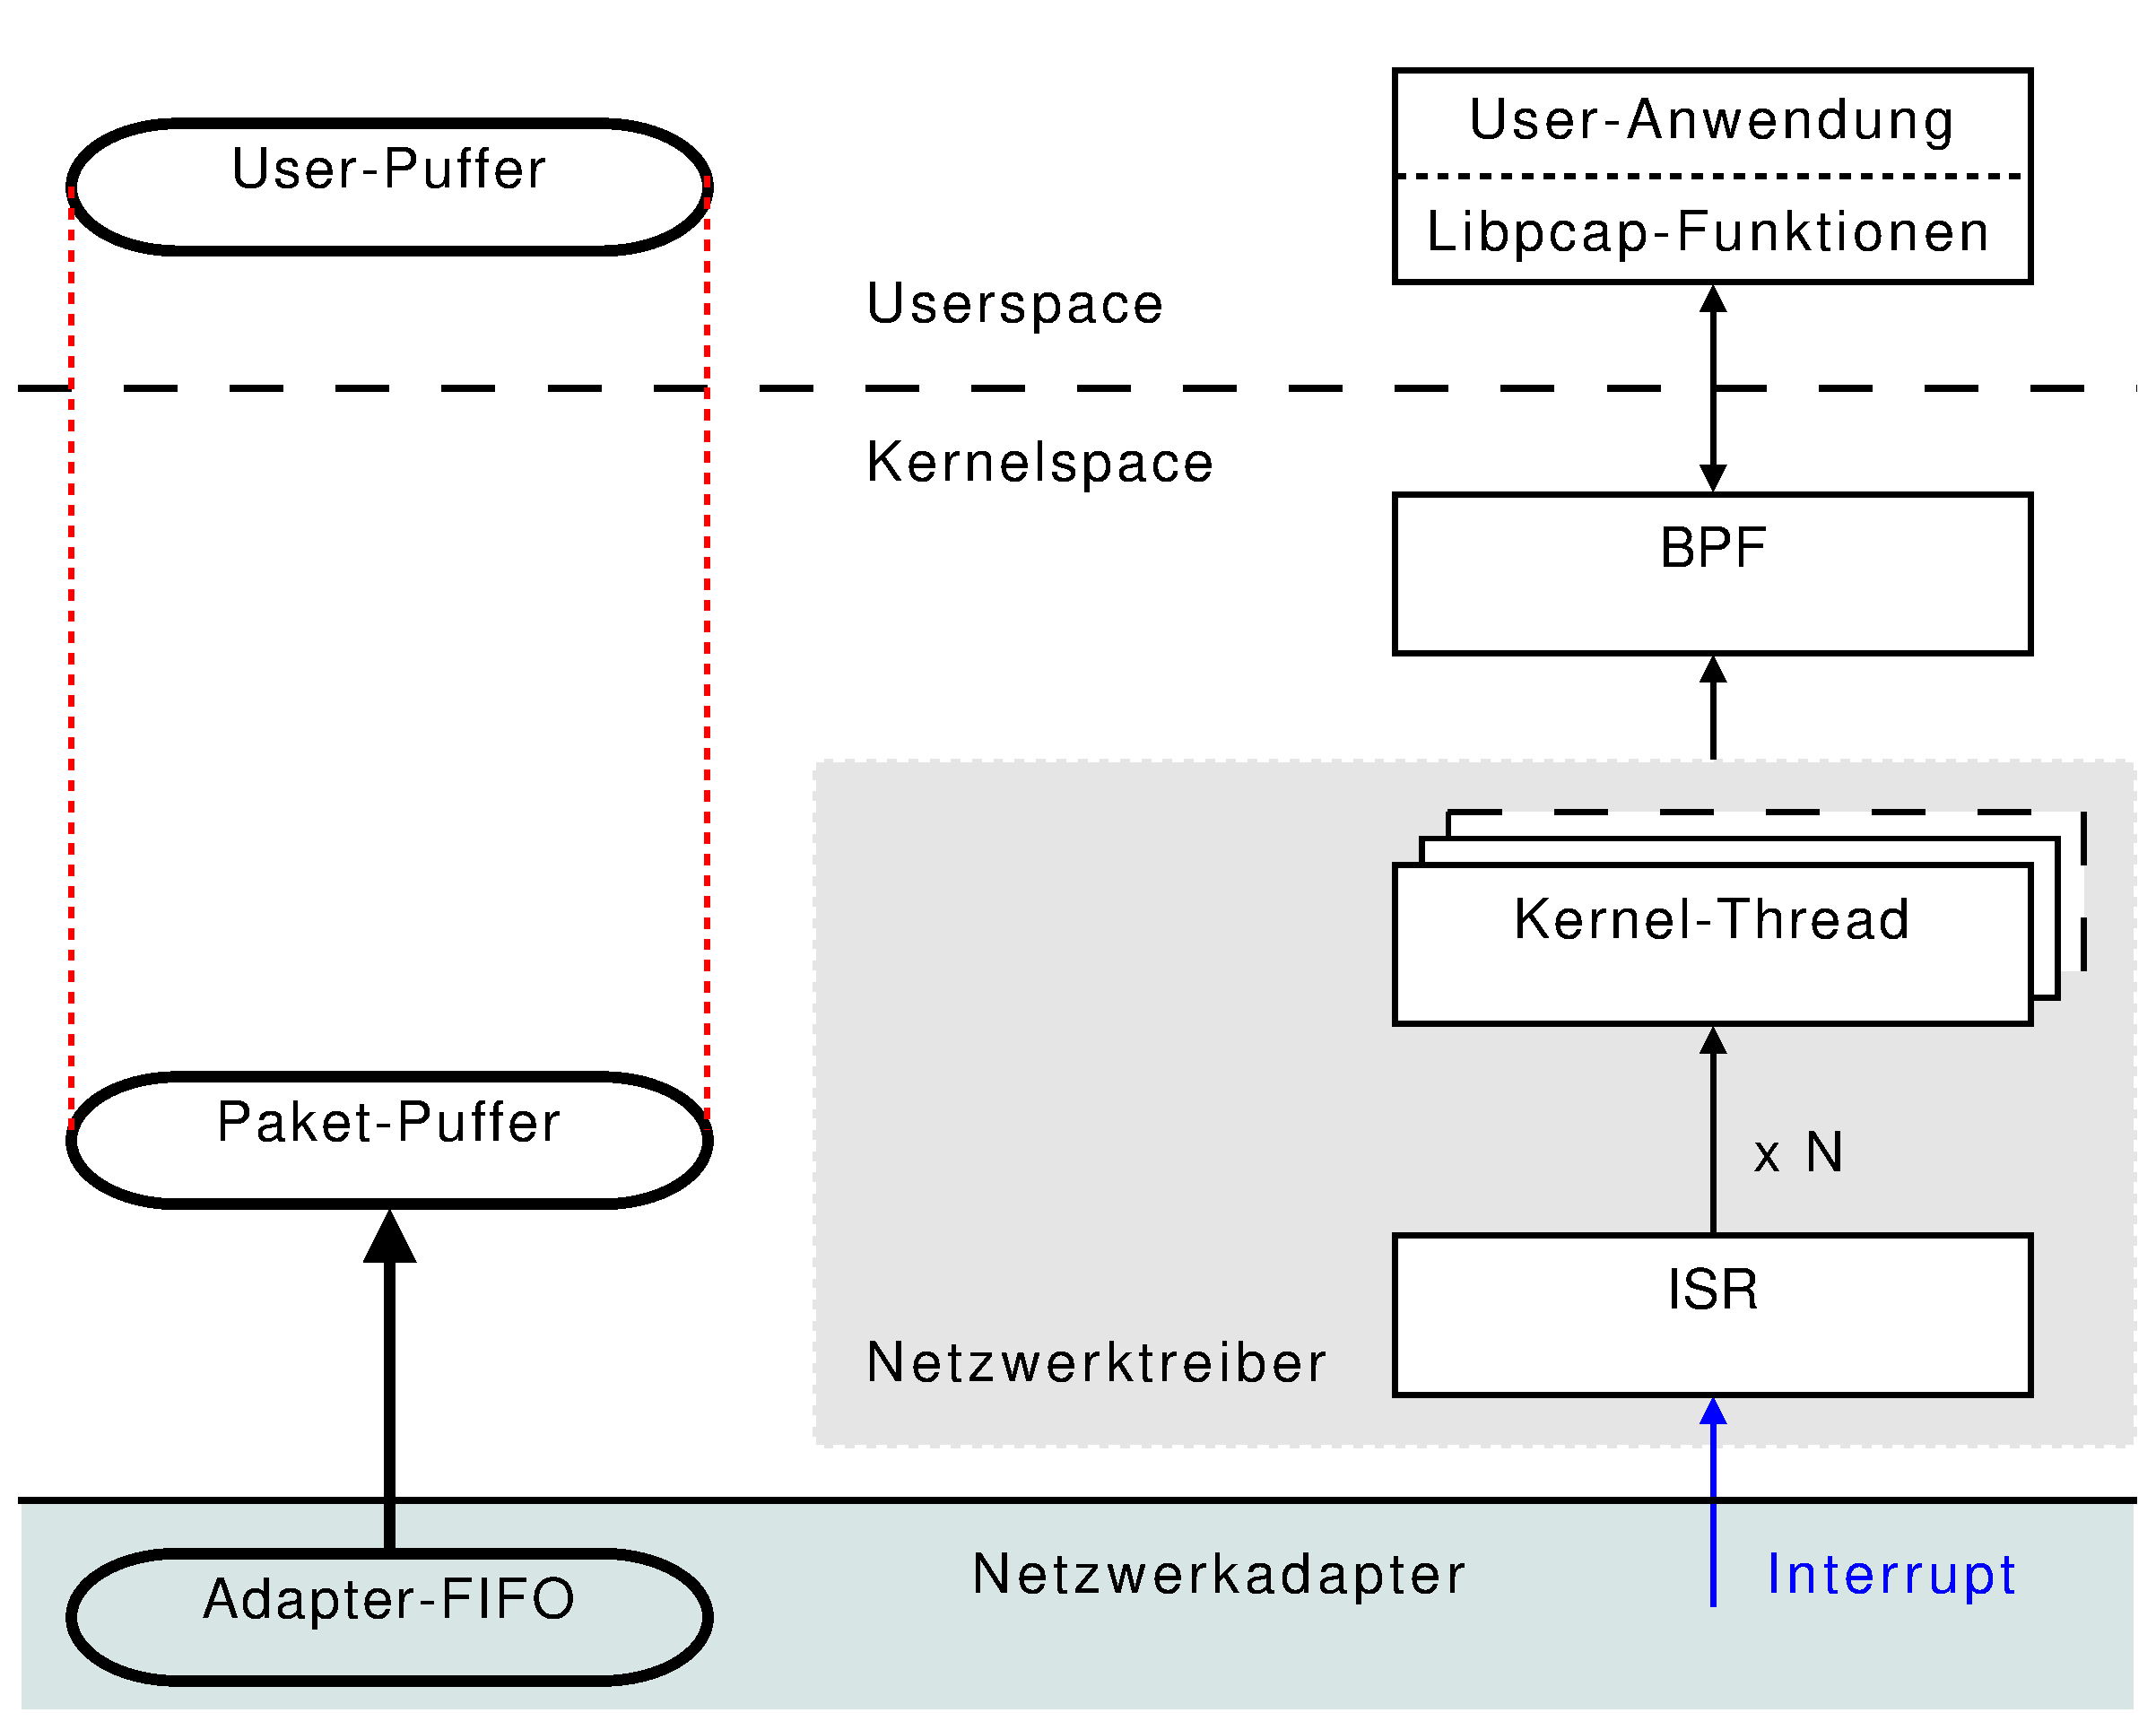
\includegraphics [height=59mm,width=60mm]{pics/3copy_solution_3}}
\only<5>{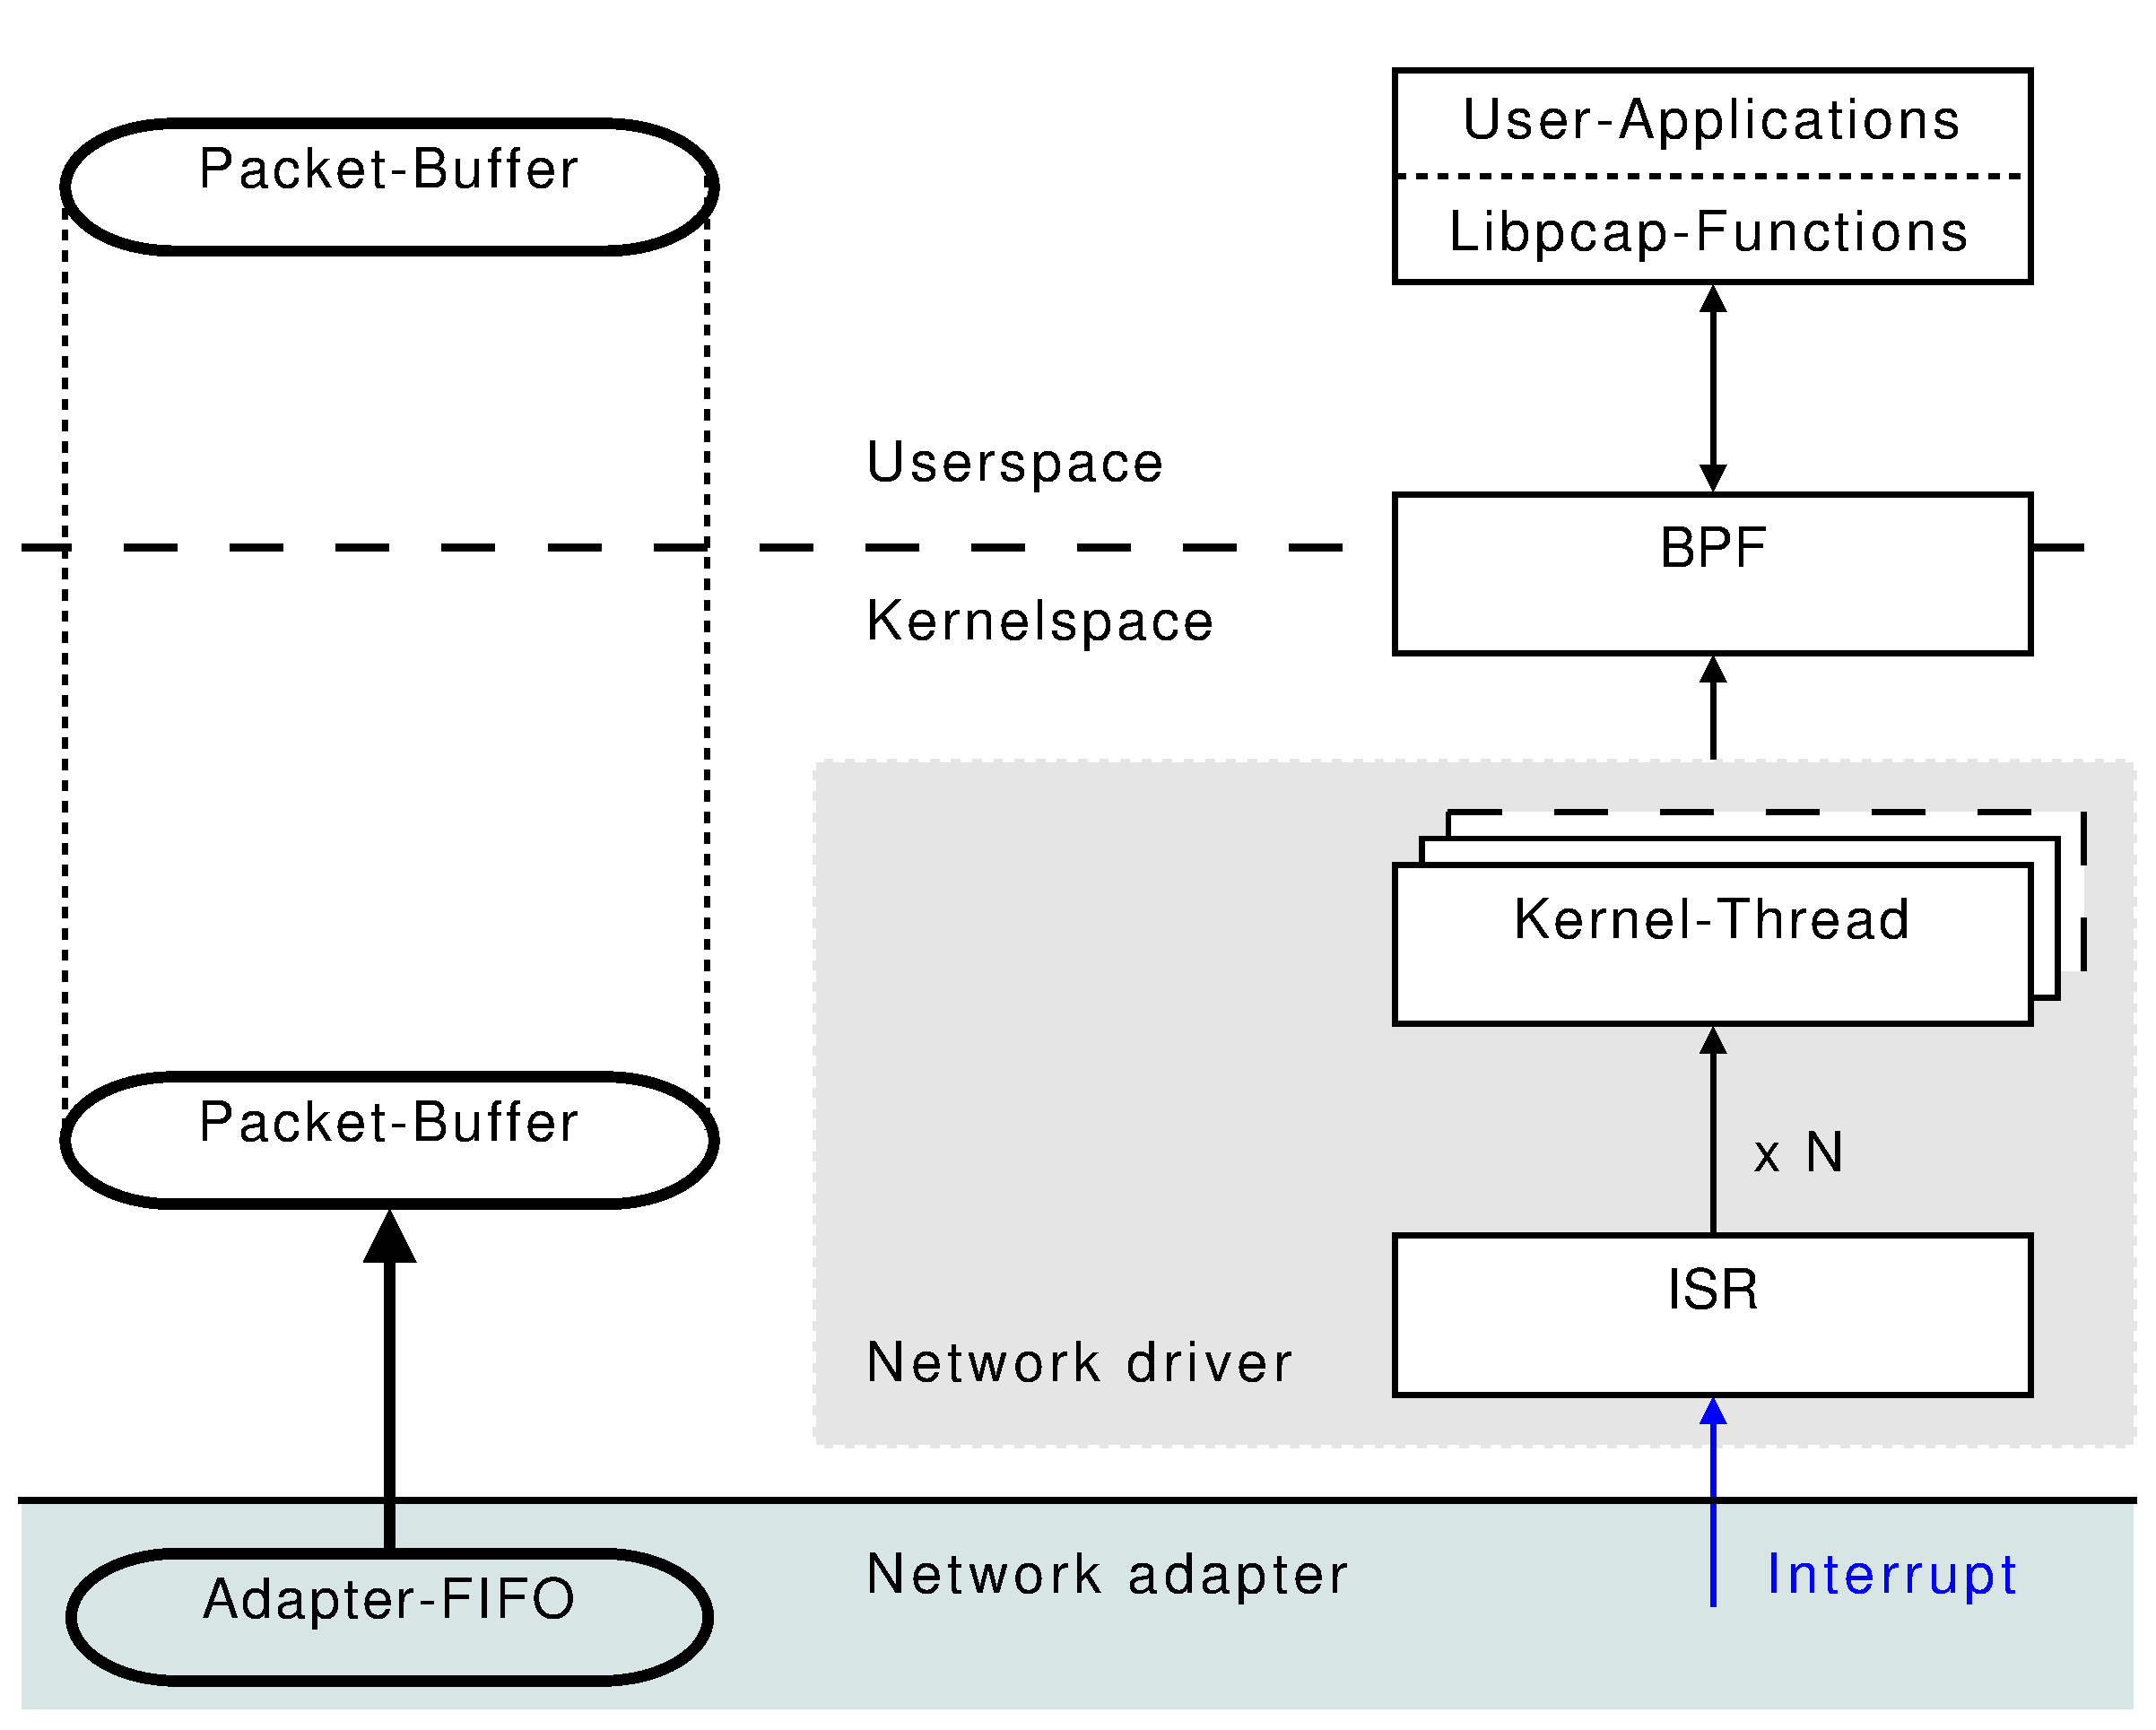
\includegraphics [height=59mm,width=60mm]{pics/3copy_solution_4}}
\only<6>{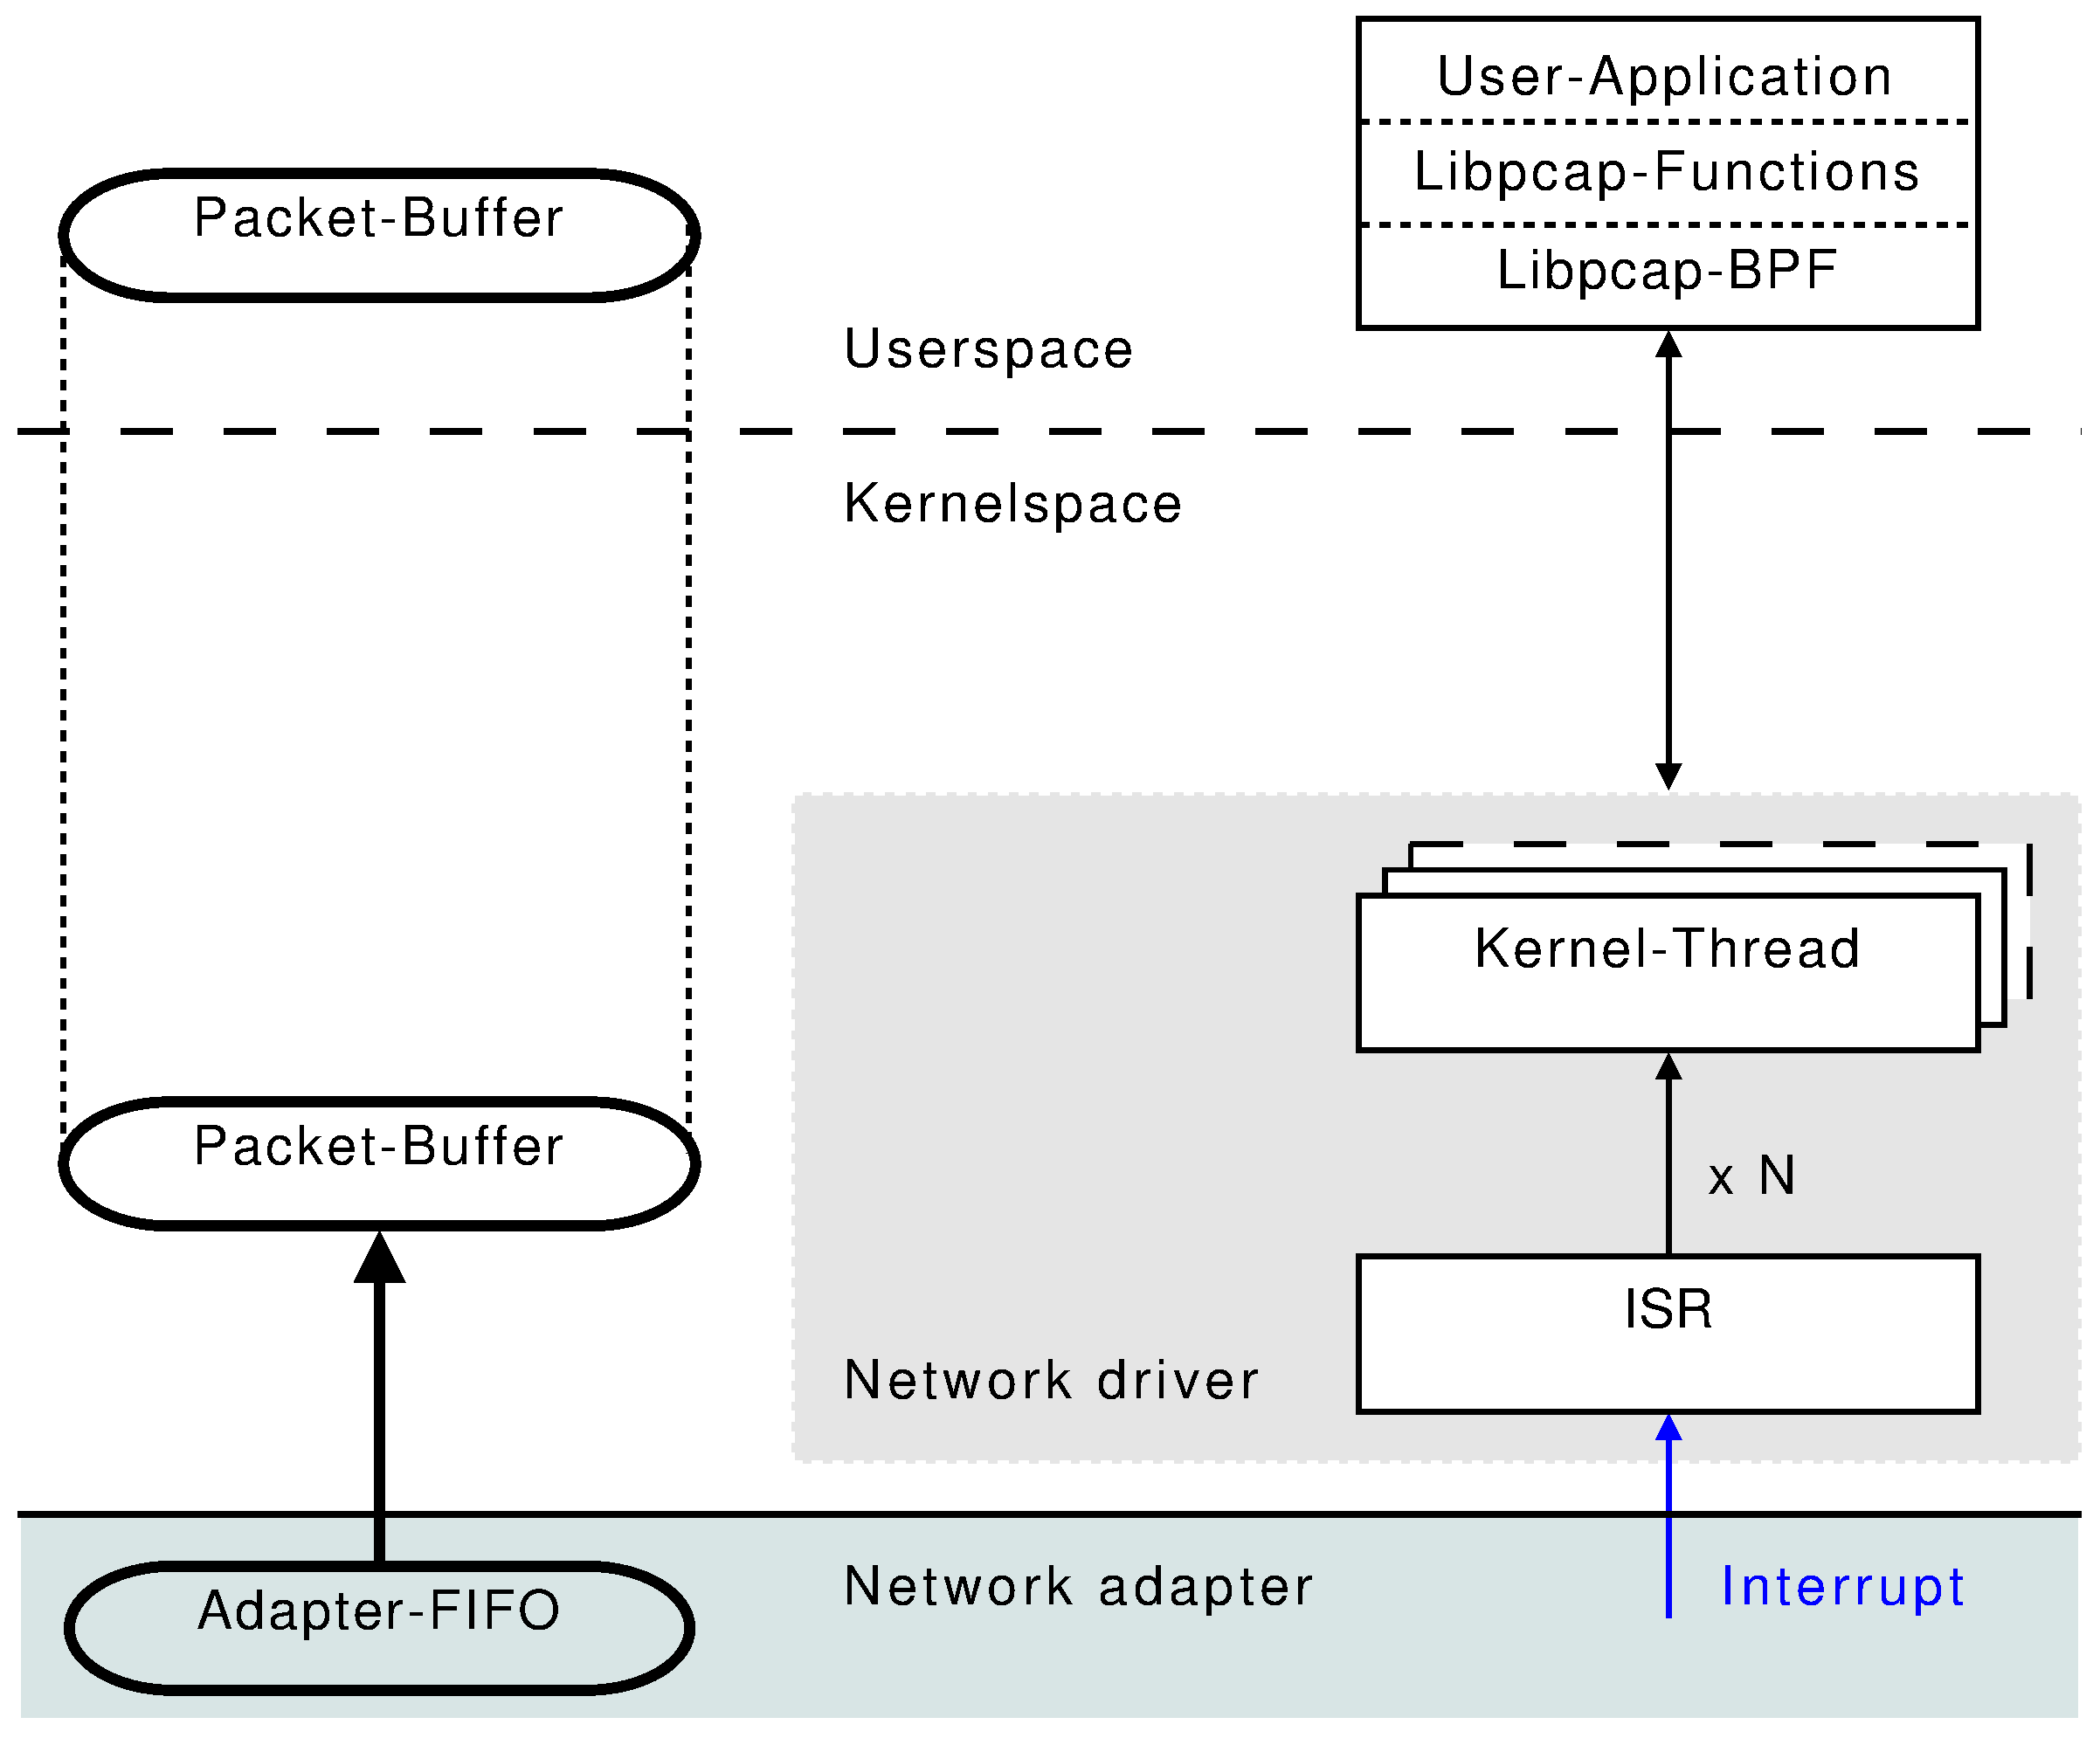
\includegraphics [height=59mm,width=60mm]{pics/3copy_solution_5}}
\end{columns}
\end{frame}

\subsection*{"Uberblick}
%%%%%%%%%%%%%%%%%%%%%%%%%%%%%%%%%%%%%%%%%%%%%%%%%%%%%%%%%%%%%%%%%%%
\begin{frame}
\frametitle{"Uberblick: Kopie-Operationen}
\begin{center}
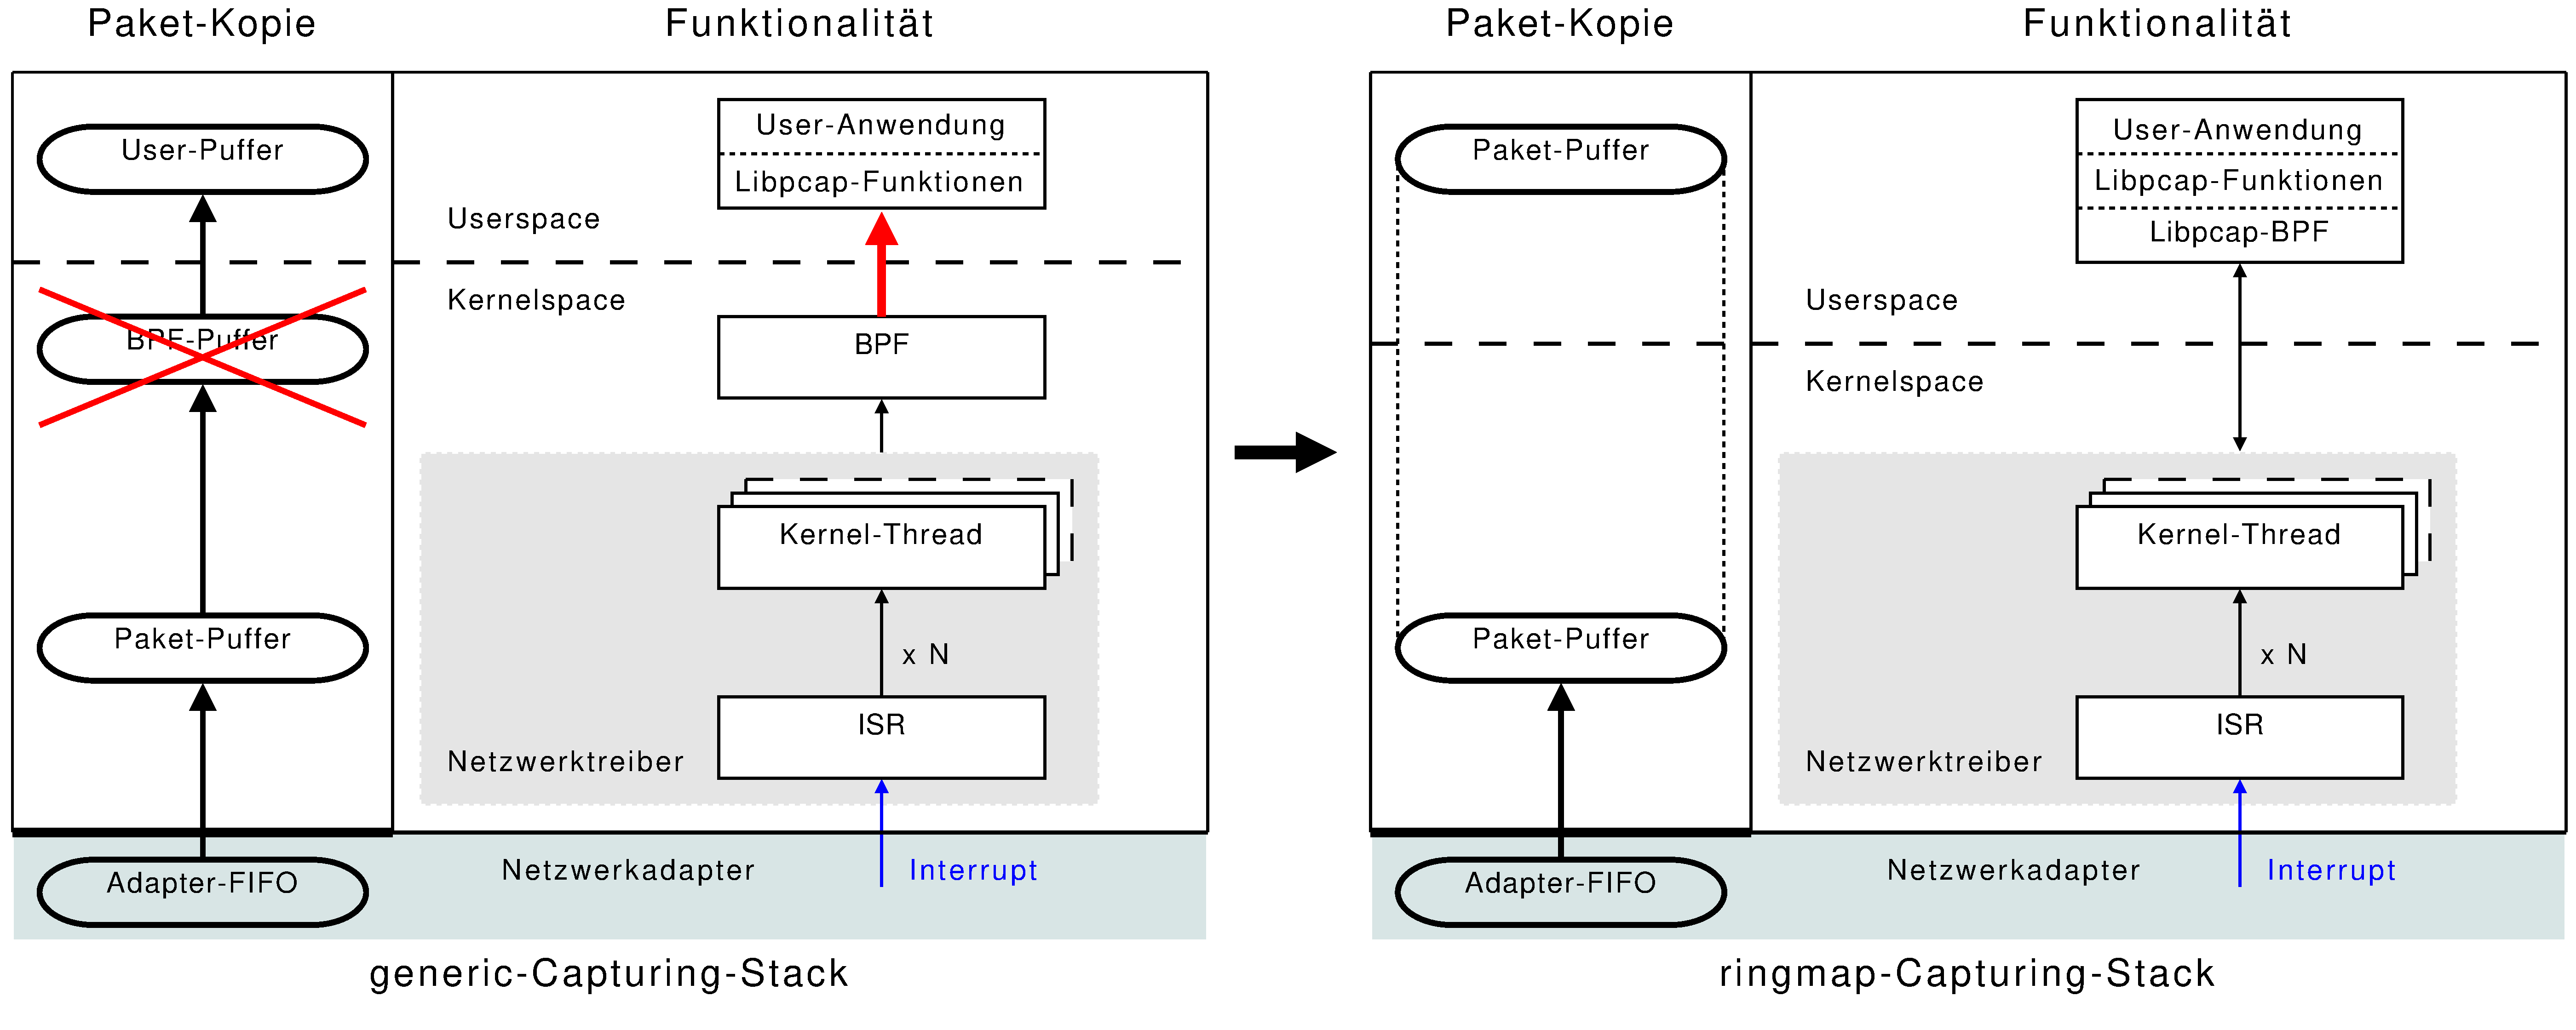
\includegraphics [height=65mm,width=115mm]{pics/Ueberblick_new}
\end{center}
\end{frame}

\section{Performance evaluation}
\begin{frame}
	\begin{center}
	\huge{Performance evaluation}
	\end{center}
\end{frame}

\subsection*{Goal of measurements}

\begin{frame}
\frametitle{Goal of measurements}
\begin{itemize}
	\item Leistungsbewertung von \textbf{ringmap}-Capturing-Stack
		\begin{itemize}
			\item CPU-Last und Paketverluste beim Capturing\newline
		\end{itemize}
	\item Leistungsvergleich: \textbf{generic} vs. \textbf{ringmap}
\end{itemize}
\end{frame}

\begin{frame}
\frametitle{Was wird gemessen ?}
Gemessen werden  die \textbf{Paketverluste} und \textbf{CPU-Last} beim
Capturing in Abh"angigkeit von unterschiedlichen:\newline
\begin{itemize}
	\item Verkehrsparameter
		\begin{itemize}
			\item Paketgr"o"se
			\item Bit-Rate bzw. Paket-Rate
		\end{itemize}

\color{gray}
	\item  Hardware-Komponenten
		\begin{itemize}
\color{gray}
			\item PCI vs. PCI-Express
			\item Anzahl der CPUs
		\end{itemize}
	\item Treiber-Parameter
		\begin{itemize}
\color{gray}
			\item Gr"o"se des Paket-Puffers
			\item etc\ldots
		\end{itemize}
\end{itemize}
\normalcolor
\end{frame}

\subsection*{Testbed}
%%%%%%%%%%%%%%%%%%%%%%%%%%%%%%%%%%%%%%%%%%%%%%%%%%%%%%%%%%%%%%%%%%%
\begin{frame}
\frametitle{Testbed}
\begin{center}
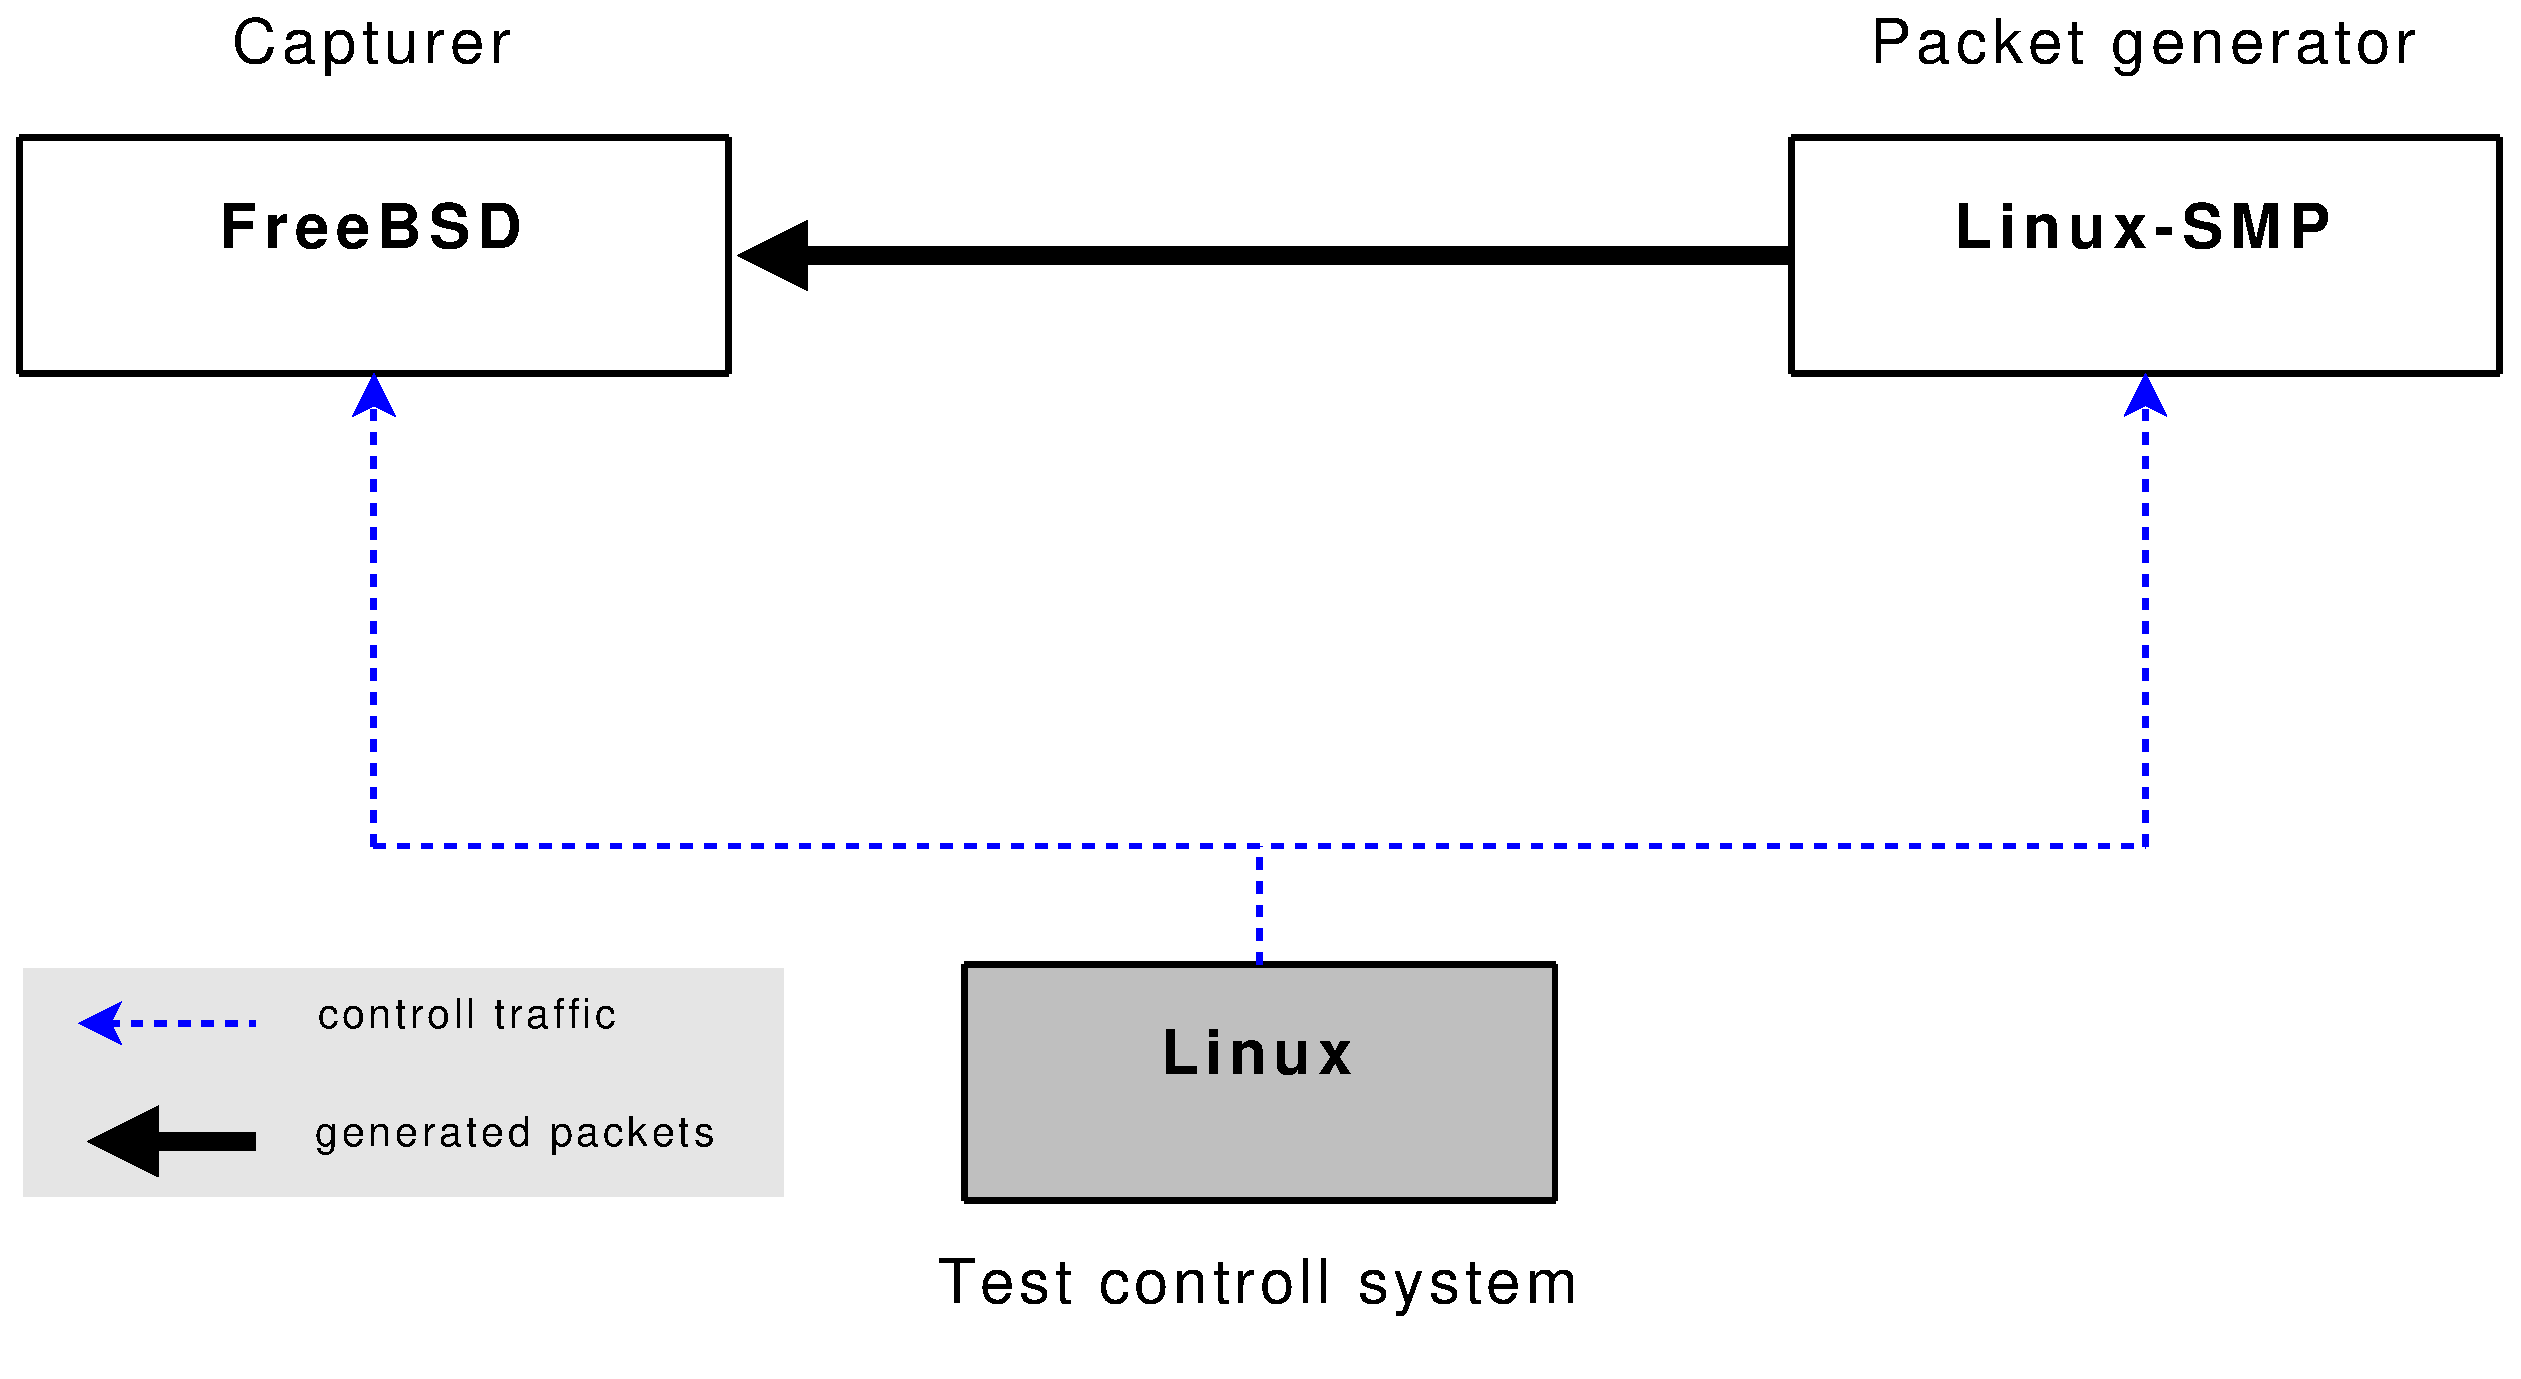
\includegraphics [height=0.68\textheight]{pics/Messaufbau}
\end{center}
\end{frame}

%%%%%%%%%%%%%%%%%%%%%%%%%%%%%%%%%%%%%%%%%%%%%%%%%%%%%%%%%%%%%%%%%%%
\begin{frame}
\frametitle{Messaufbau}
\only<1->{\textbf{Verkehrsgenerierung}}
\begin{itemize}
	\item <1->Linux Kernel Packet Generator (\emph{pktgen})
		\begin{itemize}
			\item <1->Erzeugt Verkehr mit den unterschiedlichen Charakteristiken: 
				\begin{itemize}
					\item <1->Paket-Gr"osse
					\item <1->Bit-Rate bzw. Paket-Rate
	%				\item <1->Paketenanzahl
				\end{itemize}
		\end{itemize}
\end{itemize}
\only<2->{\textbf{Capturing}}
\begin{itemize}
	\item <2->\textbf{ringmap} bzw. \textbf{generic}
	\item <2->Libpcap-Anwendung
		\begin{itemize}
			\item <2->Paketzugriff durch den Aufruf von \emph{pcap\_loop()}
			\item <2->Z"ahlen der empfangenen Pakete
		\end{itemize}
\end{itemize}
\end{frame}

\subsection*{Experimentbeschreibung}

%%%%%%%%%%%%%%%%%%%%%%%%%%%%%%%%%%%%%%%%%%%%%%%%%%%%%%%%%%%%%%%%%%%
\begin{frame}
\frametitle{Experiment-Parameter}
F"ur jedes Experiment werden Datenstr"ome mit den unterschiedlichen Parametern  erzeugt: 
\begin{itemize}
	\item Konstante Parameter: 
		\begin{itemize}
			\item Paket-L"ange
				\begin{itemize}
					\item 64, 200, 300, 700, 1500
				\end{itemize}
		\end{itemize}
	\item Variable Parameter: 
		\begin{itemize}
			\item Bit-Rate bzw. Paket-Rate
				\begin{itemize}
					\item bis $1GBit/sec$
				\end{itemize}
		\end{itemize}
\end{itemize}

\end{frame}

%%%%%%%%%%%%%%%%%%%%%%%%%%%%%%%%%%%%%%%%%%%%%%%%%%%%%%%%%%%%%%%%%%%
\begin{frame}
\frametitle{Messwerte}
\begin{itemize}
	\item System-Load
		\begin{itemize}
			\item Prozentueller Zeitanteil, den CPU im Systemmodus (\emph{protected mode}) verbringen
			\item Interrupt-Load wird nich ber"ucksichtigt
				\begin{itemize}
					\item bleibt immer gleich f"ur \textbf{generic} und \textbf{ringmap}
				\end{itemize}
			\item $syst = 1 - intr - user - nice - idle$\newline
		\end{itemize}
	\item Paketverluste 
		\begin{itemize}
			\item Differenz zwischen den gesendeten und empfangenen Paketen
			\item $Pakete_{loss} = Pakete_{send} - Pakete_{received}$
		\end{itemize}
\end{itemize}
\end{frame}

\subsection*{Ablauf des Experiments}
%%%%%%%%%%%%%%%%%%%%%%%%%%%%%%%%%%%%%%%%%%%%%%%%%%%%%%%%%%%%%%%%%%%
\begin{frame}
\frametitle{Ablauf des Experiments}
\begin{enumerate}
	\item \textbf{Starten des Capturing-Prozesses:}
		\begin{itemize}
			\item Starten System-Last-Messung
		\end{itemize}
	\item \textbf{Generieren des Verkehrs:}
		\begin{itemize}
			\item mit einer bestimmten Paketmenge
			\item mit einer bestimmten Bit-Rate bzw. Paket-Rate
		\end{itemize}
	\item \textbf{Stop Capturing- und Messung-Prozess}
	\item \textbf{Speicherung der gemessenen Werte}
\end{enumerate}
\begin{itemize}
	\item Jedes Experiment wird f"unf mal wiederholt
	\item Die \emph{Mittelwerte} und \emph{Standardabweichung} wird berechnet
\end{itemize}
\end{frame}

\subsection*{Probleme bei Experimenten}
%%%%%%%%%%%%%%%%%%%%%%%%%%%%%%%%%%%%%%%%%%%%%%%%%%%%%%%%%%%%%%%%%%%
\begin{frame}
\frametitle{Probleme bei Experimenten}
\begin{itemize}
	\item Unstabilit"at des Linux-Kernel-Packet-Generator
		\begin{itemize}
			\item Kernel panics beim Generieren gro"sen Paketmengen 
			\item [$\Rightarrow$] deswegen maximal $15000000 pkts$ pro Experiment\newline
		\end{itemize}
	\item Unm"oglich einen Verkehr mit einer beliebigen Paket- bzw. Bit-Rate zu erzeugen
		\begin{itemize}
			\item Aufgrund von Interrupt-Throttling auf dem Paketgenerator-System
			\item [$\Rightarrow$] deswegen nur bestimmte Messpunkte m"oglich\newline
		\end{itemize}
	\item Flow-Control
		\begin{itemize}
			\item begrenzt die Rate des erzeugten Verkehr
			\item muss vor den Testabl"aufen abgeschaltet werden
		\end{itemize}
\end{itemize}
\end{frame}

\subsection*{Ergebnisse}
\begin{frame}
	\begin{center}
	\huge{Ergebnisse}
	\end{center}
\end{frame}
%%%%%%%%%%%%%%%%%%%%%%%%%%%%%%%%%%%%%%%%%%%%%%%%%%%%%%%%%%%%%%%%%%%
\begin{frame}
\frametitle{generic vs. ringmap: Paketverluste}
\begin{center}
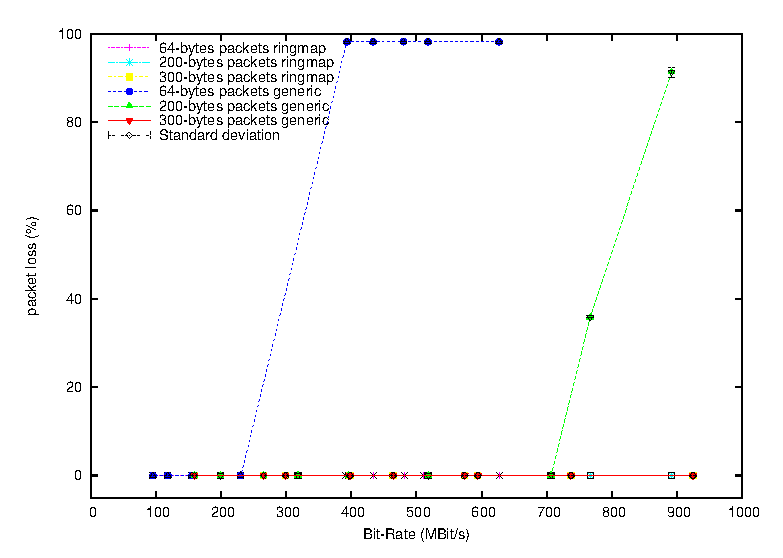
\includegraphics [height=0.81\textheight]{plots/pktloss_generic_vs_ringmap_mbs.eps}
\end{center}
\end{frame}

%%%%%%%%%%%%%%%%%%%%%%%%%%%%%%%%%%%%%%%%%%%%%%%%%%%%%%%%%%%%%%%%%%%
\begin{frame}
\frametitle{generic vs. ringmap: Systemload}
\begin{center}
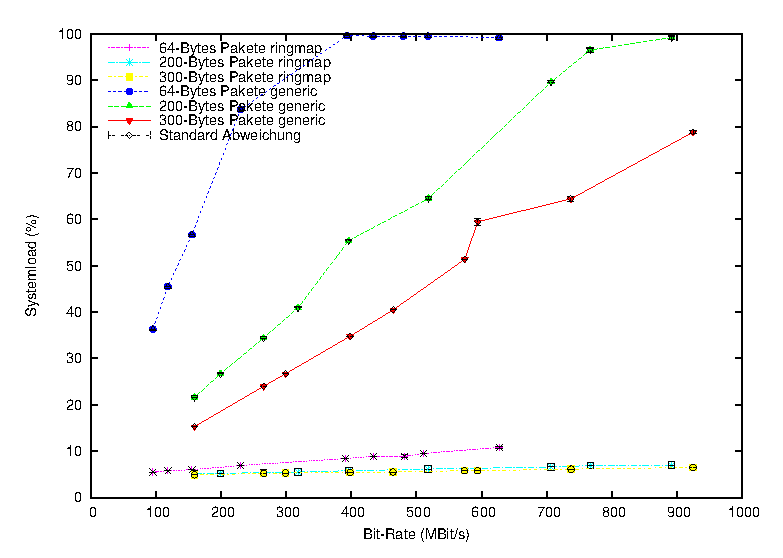
\includegraphics [height=0.81\textheight]{plots/sysload_generic_vs_ringmap_mbs.eps}
\end{center}
\end{frame}

\section{Summary}
\begin{frame}
	\begin{center}
	\huge{Summary}
	\end{center}
\end{frame}
%%%%%%%%%%%%%%%%%%%%%%%%%%%%%%%%%%%%%%%%%%%%%%%%%%%%%%%%%%%%%%%%%%%
\begin{frame}
\frametitle{Achieved goals}
\begin{itemize}
	\item Verbesserung der Capturing-Performance
		\begin{itemize}
			\item Sehr geringe Systemload (unter $12\%$) und sehr kleine
				Paketverluste (unter  $0.02\%$)
				\begin{itemize}
					\item nur bei der Erfassung der kleinsten 64-Bytes-Pakete
					\item nur bei maximal erreichte Paket-Rate ("uber $450000 pkts/sec$) 
				\end{itemize}
		\end{itemize}
	\item Stabilit"at und Benutzbarkeit der implementierten Software
		\begin{itemize}
			\item W"ahrend aller Tests keine \emph{kernel panics}, \emph{segmentation faults}, etc\ldots
			\item Sehr einfache Einsetzbarkeit
				\begin{itemize}
					\item Zwei Shell-Skripte zum Installieren bzw. Deinstallieren des 
						\emph{ringmap}-Capturing-Stacks
				\end{itemize}
			\item Jede Libpcap-Anwendung ist benutzbar
		\end{itemize}
\end{itemize}
\end{frame}

\begin{frame}
\frametitle{Future works}
\begin{itemize}
	\item Performance-Vergleich mit FreBSD-8.x
		\begin{itemize}
			\item W"ahrend der Lauf der Diplomarbeit war in Alpha-Stadium\newline
		\end{itemize}
	\item 10-GBit-Paket-Capturing
		\begin{itemize}
			\item Der Treiber f"ur Intel-Netzwerkadpter f"ur 10-Gigabit-Netzwerkanschlüsse hat 
				eine "ahnliche Struktur und sollte sich portieren lassen. 
		\end{itemize}
\end{itemize}
\end{frame}

%\begin{frame}
%\frametitle{Weg eines Paketes. Hardware View}
%\begin{columns}
%\column[t]{0.5\textwidth}
%\vspace{-17em}
%\begin{enumerate}
%	\item Paketenempfang
%		\begin{itemize}
%			\item Datentransfer "uber PCI
%			\item meistens DMA-gesteuert
%		\end{itemize}
%	\item Paketenauswertung und Filtern
%		\begin{itemize}
%			\item Mehrfacher Datentransfer zwischen RAM und CPU
%		\end{itemize}
%	\item Paketenaufzeichnung
%		\begin{itemize}
%			\item Ausgabe auf Terminal
%			\item Datenspeicherung auf Hintergrundspeicher
%			\item Wird nicht im Rahmen der DA analysiert.
%		\end{itemize}
%\end{enumerate}
%\column[t]{0.5\textwidth}
%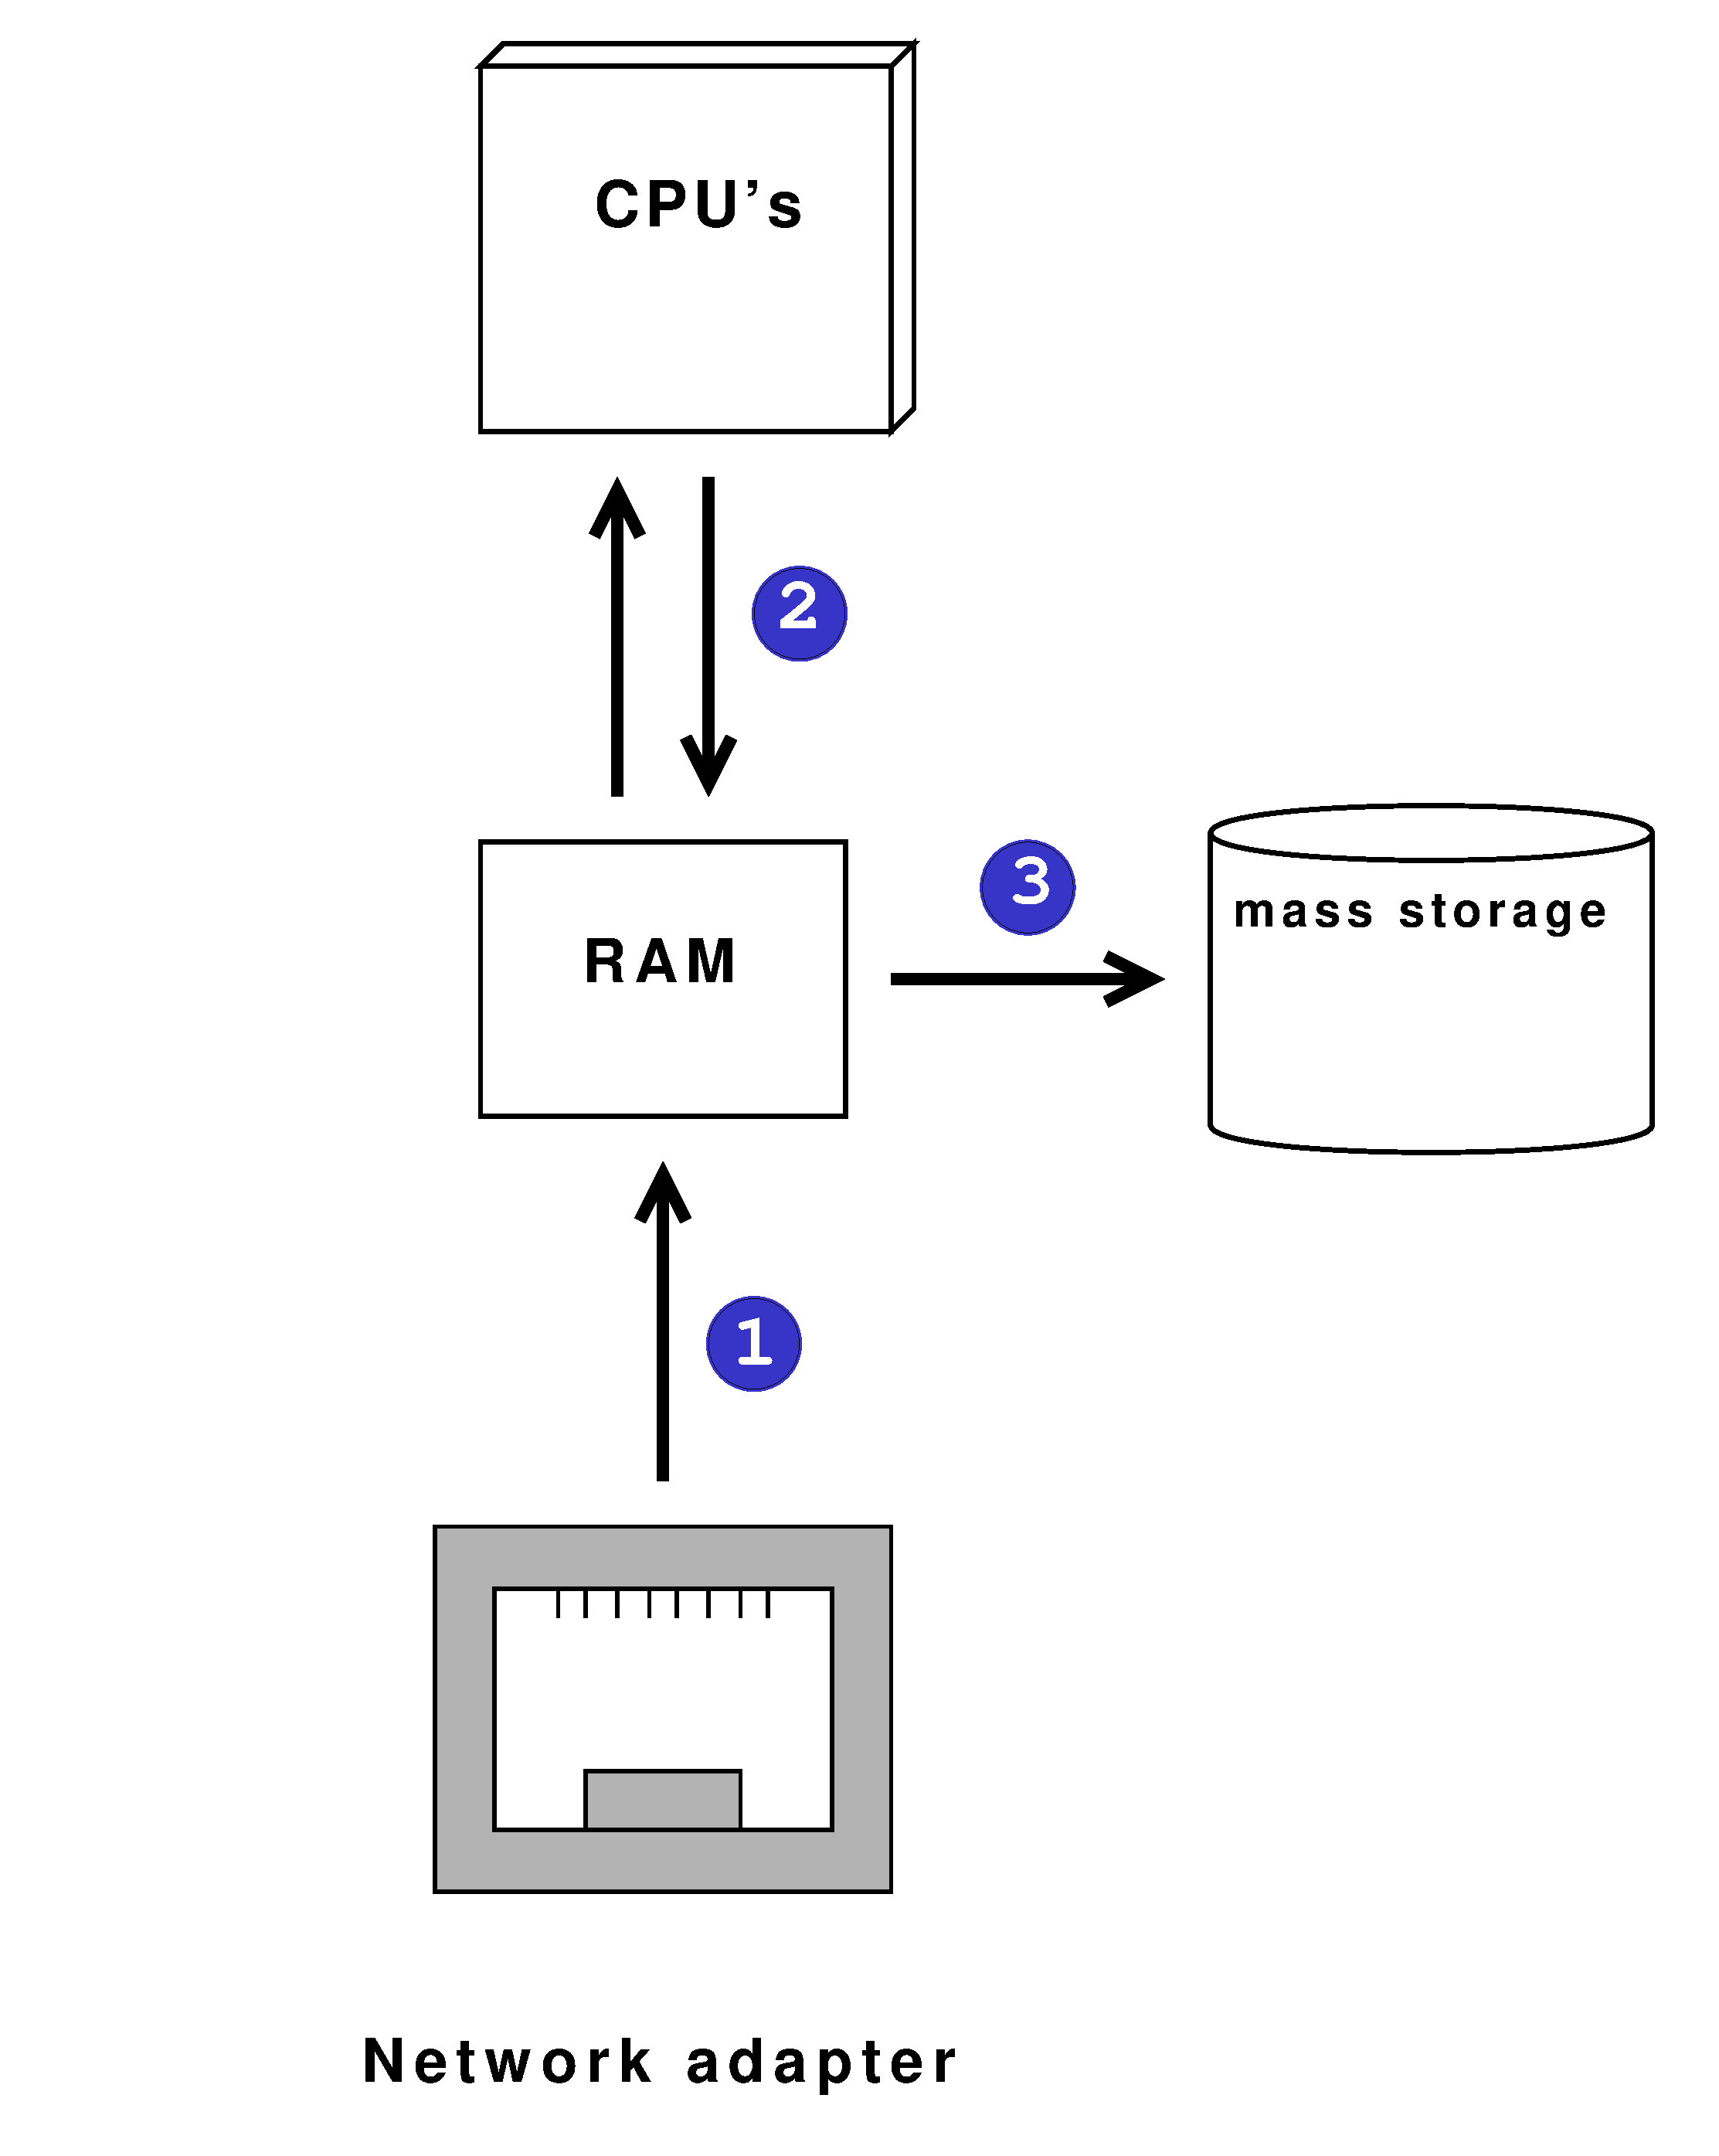
\includegraphics [width=0.90\textwidth, keepaspectratio]{pics/HardwareView}
%\end{columns}
%\end{frame}
%
%
%\begin{frame}
%\frametitle{Weg eines Paketes. Generic-Capturing-Stack}
%\begin{columns}
%\column[t]{0.5\textwidth}
%\vspace{-14em}
%\begin{enumerate}
%	\item Paketenempfang
%		\begin{itemize}
%			\item Datenkopieren:\newline 
%				\textbf{Netzwerk} \textrightarrow \textbf{NIC} \textrightarrow \textbf{RAM} \newline 
%		\end{itemize}
%	\item  Paketfilterung
%		\begin{itemize}
%		\item BPF Code anwenden\newline
%		\item Datenkopieren: \newline 
%			\textbf{Paket-Puffer} \textrightarrow \textbf{BPF-Puffer} \newline 
%		\item Datenkopieren: \newline
%			\textbf{BPF-Puffer} \textrightarrow \textbf{User-Puffer}
%		\end{itemize}
%\end{enumerate}
%
%	\column[t]{0.5\textwidth}
%	%\vspace{-20em}
%	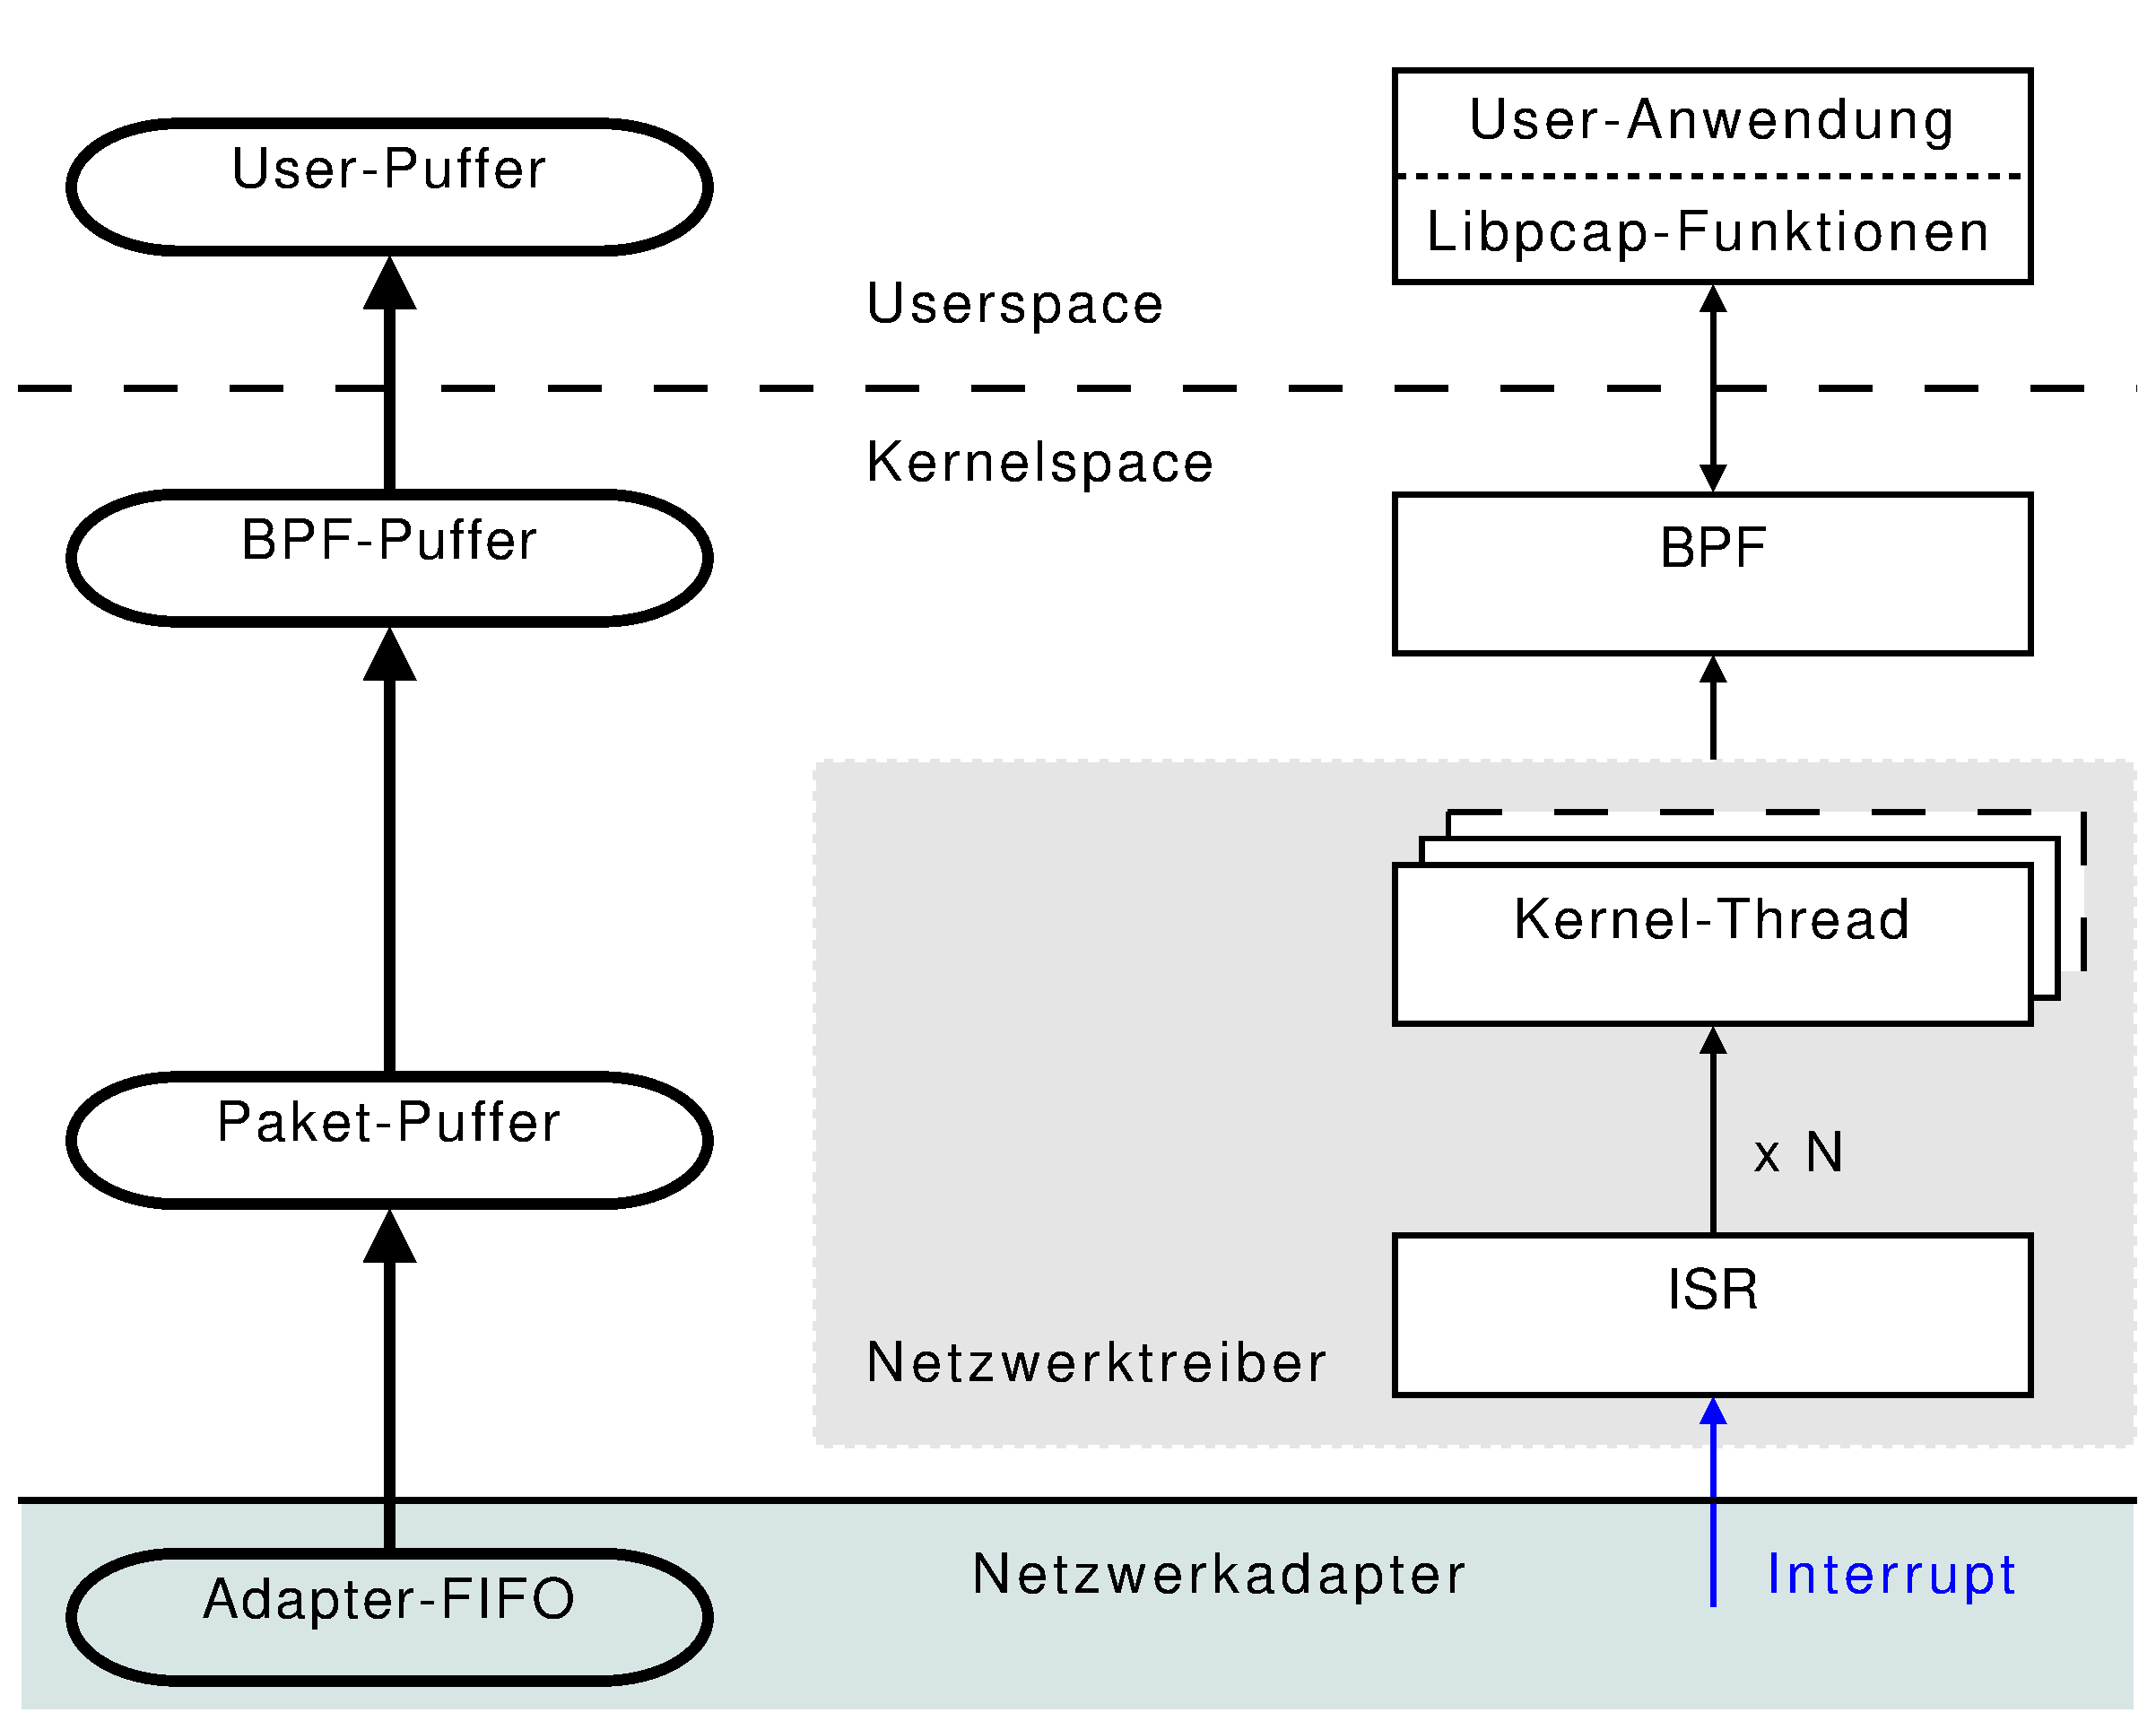
\includegraphics [height=0.61\textheight]{pics/3copy}
%	\end{columns}
%
%\end{frame}
%
%
%\begin{frame}
%\frametitle{M"ogliche Ursachen des Paketverlustes}
%\begin{itemize}
%	\item Nicht ausreichende effektive Bandbreiten der internen Bussen: PCI-Bussystem, Speicherbus
%			% \begin{quota}
%			%	Effektive Datentransferraten interner Bussen eines Rechnersystem sind 
%			%	meistens (wesentlich) geringer als ihre maximale theoretische Werte.	
%			%	Die Ursachen daf"ur:
%	\begin{itemize}
%		\item 	Wartezyklen
%		\item	Overhead beim Lesen und Schreiben: 
%					Arbitering, Handshaking, etc \ldots
%	\end{itemize}
%\end{itemize}
%\begin{itemize}
%		\item Hohe Interrupt-Load 
%			\begin{itemize}
%			\item Hohe Paketrate $\Rightarrow$ Hohe Interrupt-Rate $\Rightarrow$ 
%					\emph{Receive Interrupt Livelock} 
%			\end{itemize}
%\end{itemize}
%\end{frame}
%
%
%\begin{frame}
%\frametitle{Effektive Bandbreiten der internen Bussen.\newline PCI-Bussystem}
%	%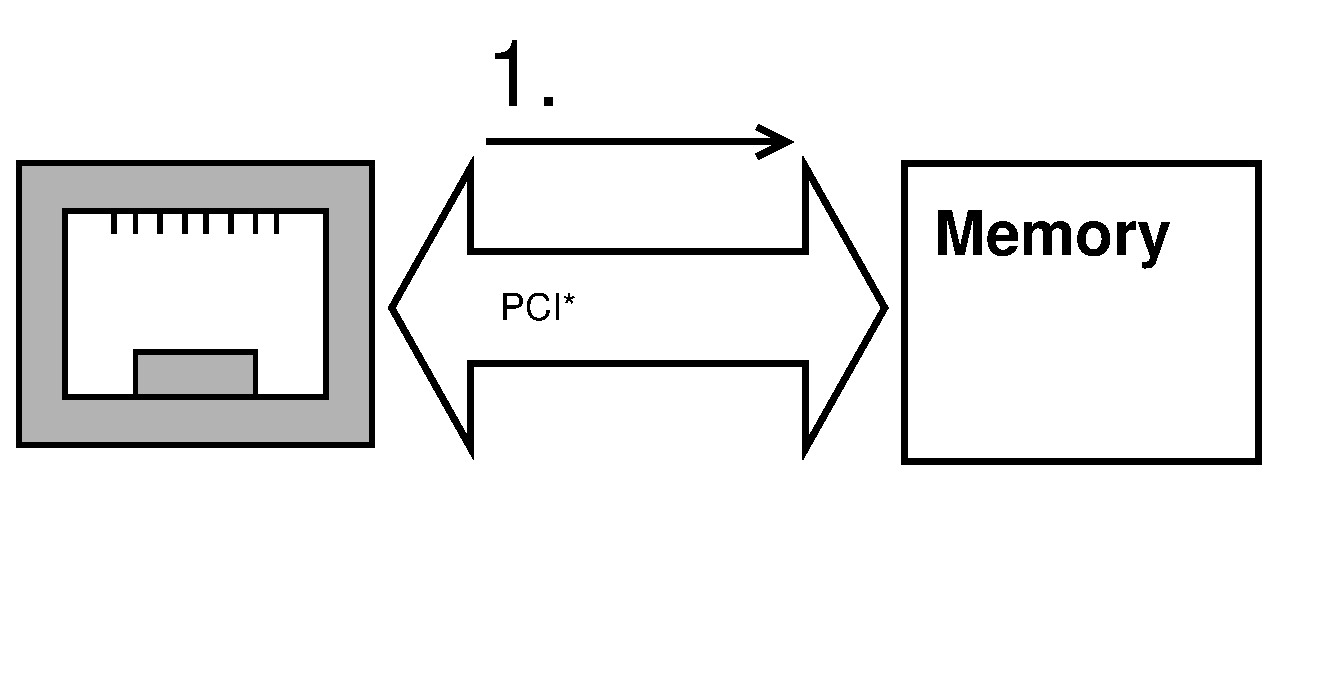
\includegraphics [width=0.25\textwidth, keepaspectratio]{pics/pcibushw}
%\begin{itemize}
%	\item 	PCI, PCI-X
%		\begin{itemize}
%			\item 	Shared Bus-System $\Rightarrow$ 
%					keine deterministischen Datentransferraten
%			\item 	u.U, zum Beispiel, bei mehreren Ger"aten an einem Bus 
%					kann beim Datentransfer $\geq1$Gbit/s ein Flaschenhals werden
%		\end{itemize}
%\end{itemize}
%\begin{itemize}
%				\item	PCI-Express
%					\begin{itemize}
%					\item	Garantierte effektive Bandbreite
%% theoretische Übertragungsrate bei 2,5-GHz-Takt: 250 MByte/s netto pro Lane und Richtung
%					\item	bei der entsprechenden Anzahl an Lanes hat ausreichende 
%							Performance f"ur 10Gbit/s Datentransferrate 
%					\end{itemize}
%\end{itemize}
%\end{frame}
%
%
%\begin{frame}
%\frametitle{Effektive Bandbreiten der internen Bussen.\newline Speicherbus}	
%	Effektive Speicherbandbreite kann mit Hilfe von Benchmarks gemessen werden: 
%	Stream, lmbench, etc \ldots \newline \\ 
%	%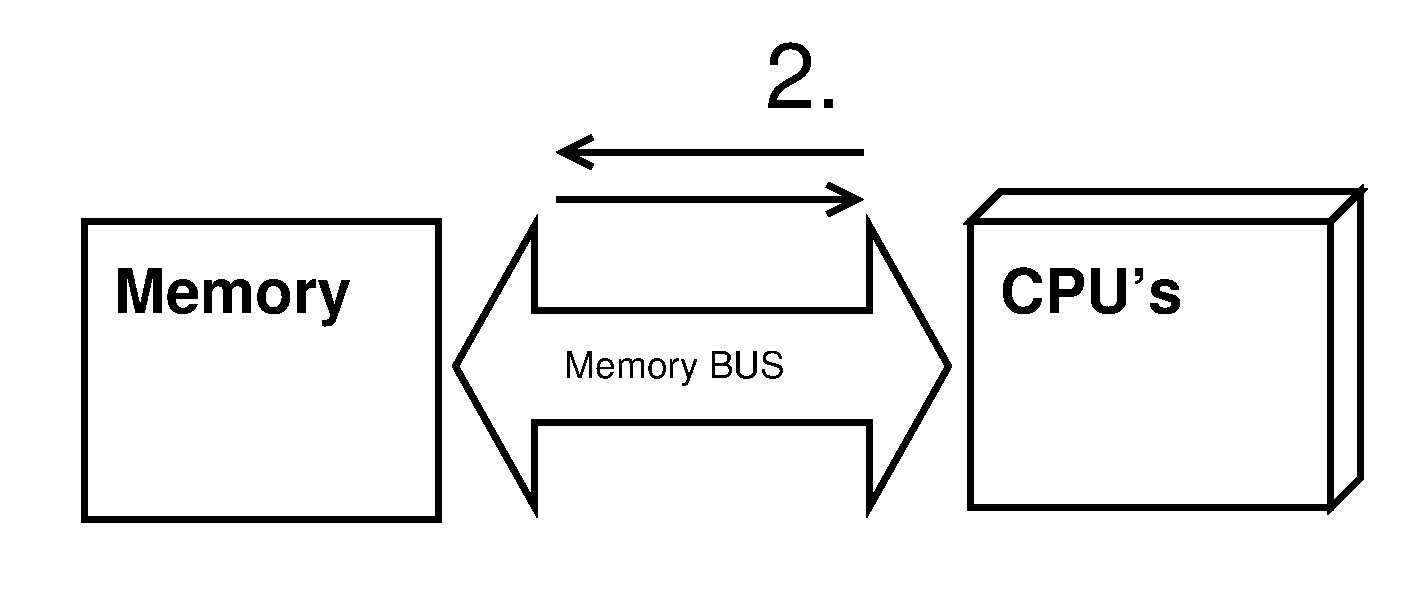
\includegraphics [width=0.25\textwidth, keepaspectratio]{pics/ramtocpuhw}
%	\begin{itemize}
%	\item	STREAM Benchmark: ein synthetischer Benchmark f"ur Ermittlung  des Durchsatzes des 
%			Hauptspeichers.
%		\begin{itemize}
%		\item 	Es wird den maximalen Datendurchsatz gemessen, den ein System bei Verwendung 
%				von Standard-Software "uber l"angere Zeit in der Praxis aufrechterhalten kann
%		\item 	Z"ahlt jeden Byte-Transfer: vom Speicher zur CPU (read) + 
%				von CPU zum Speicher (write)
%		\item 	Das Ergebnis von Stream ist c.a. das Doppelte von \textit{bcopy}
%				%	For the simple "Copy" kernel, this is exactly twice the 
%				%	number obtained from the "bcopy" convention
%		\end{itemize}
%	\end{itemize}	
%\end{frame}
%
%
%\begin{frame}
%\frametitle{Effektive Bandbreiten der internen Bussen.\newline Speicherbus}		
%	{\footnotesize
%	\begin{center}
%	\begin{table}
%	\caption{\tiny Speicherbandbreiten (MB/sec) bei STREAM benchmark mit P threads}
%	\begin{tabular}{|c|c|c|l||c|c|c|}												\hline
%
%	Mem     &	CPU 		 & ncpus & RAM	dual ch.&P=1   & P=2 	&P=4  	\\	\hline \hline
%	-		&Athlon 64 2.2GHz&	 1	 & PC-4200 		&2020  &	-   & -	 	\\	\cline{1-7}	
%	UMA     &Intel P4 3GHz	 &   2	 & PC-4200 		&2780  & 2640  	& -		\\	\cline{1-7}
%	NUMA	&Opteron  244	 &	 2 	 & PC-2700 		&2350  & 4040 	& -     \\	\cline{2-7}
%			&Opteron  848 	 &	 4	 & PC-3200 	 	&4450  & 8740	& 15400	\\	\hline
%	\end{tabular}
%	\end{table}
%	\end{center}
%	}
%	
%	\begin{itemize}
%	\item Effektive Bandbreite meistens $<50\%$ des max. theoretischen Wertes
%	\item UMA (SMP)
%		\begin{itemize}
%			\item Nicht skalierbar: Anzahl von CPUs bzw. Threads hat fast kein 
%				positives Effekt auf Speicherbandbreite
%		\end{itemize}
%	\item NUMA
%		\begin{itemize}
%		\item 	Skalierbar: Je mehr CPUs, desto gr"oser Speicherbandbreite
%		\item 	H"ohere Datentransferrate ist nur mit der gr"osseren  Anzahl von Threads m"oglich
%		\end{itemize}
%	\end{itemize}
%\end{frame}
%
%
%\begin{frame}
%\frametitle{Effektive Bandbreiten der internen Bussen.\newline Speicherbus}
%	\begin{columns}
%	\column[t]{0.7\textwidth}	
%	\vspace{-15em}
%	\begin{itemize}
%	\item $3 \times Copy\equiv 5 \times Datentransfer$
%		\begin{itemize}
%			\item Paketenempfang: NIC\textrightarrow RAM (1)
%			\item Filtern: 
%				\begin{itemize}
%					\item Copy in BPF-Puffer: RAM\textrightarrow RAM (2,3)
%					\item Copy in User-Puffer: RAM\textrightarrow RAM (4,5)
%				\end{itemize}
%		\end{itemize}
%	\item Herausforderung: $1 GBit/s$ zu capturen
%		\begin{itemize}
%		\item $\Rightarrow 5 \times 1GBit \approx 670 MByte/s$ 
%		\end{itemize}
%	\item $10 GBit/s$ zu capturen
%		\begin{itemize}
%			\item $\Rightarrow 5 \times 10GBit \approx 6.7GByte/s$
%		\end{itemize}
%	\item Problem: Zu viele Copy-Operationen!
%	\end{itemize}
%
%	\column[t]{0.3\textwidth}
%	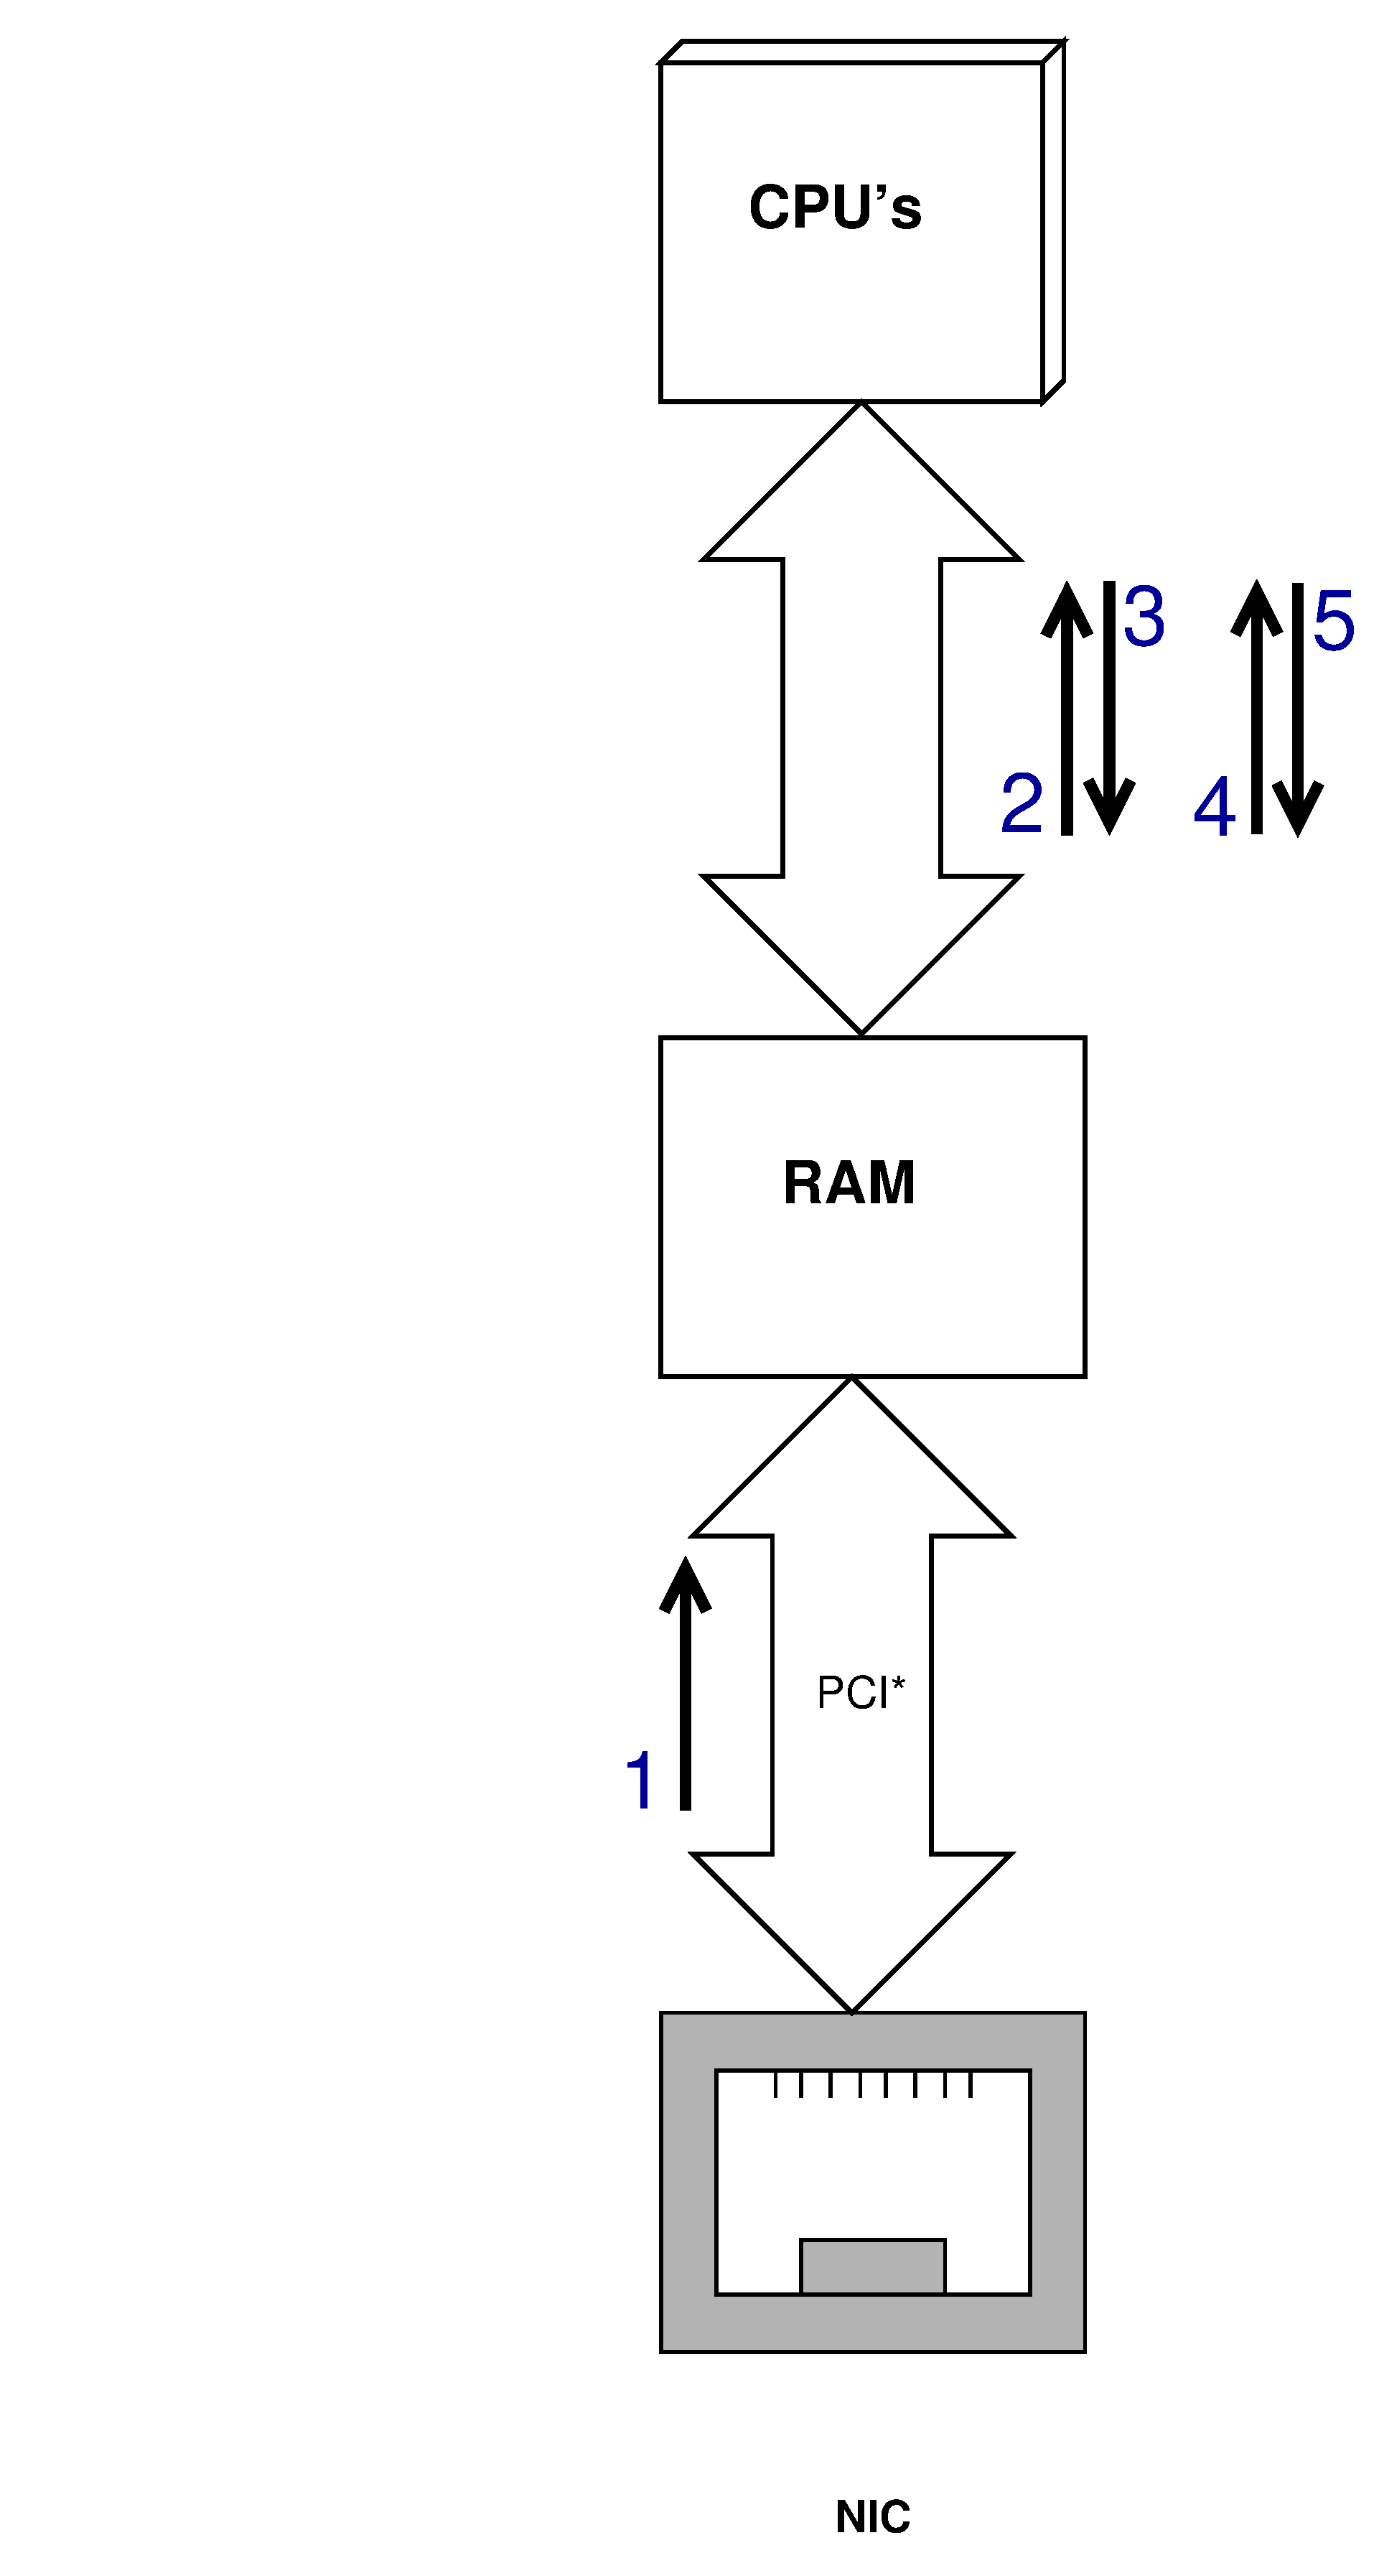
\includegraphics [width=0.90\textwidth, keepaspectratio]{pics/HardwareView_part}
%	\end{columns}
%\end{frame}
%
%
%\begin{frame}
%\frametitle{Interrupt-Load}
%	\textit{Receive Livelock} Problem \newline \\
%	\begin{itemize}
%	\item Hohe Paketrate $\Rightarrow$ hohe Interrupt-Load
%	\item $1 GBit/s = 1073741824 Bit/s$, Cycles per Interrupt $\geq 1000$,\newline 
%		ein Interrupt pro Paket:\newline
%		\begin{itemize}
%		\item Paketgr"osse $1500 Bytes = 120 000 Bit$ 
%			\begin{itemize}
%			\item $Paketrate = 1073741824\div120000 = 89478 pps$
%			\item $\Rightarrow Cycles \geq 89\ 478\ 000/s$
%			\end{itemize}
%		\item Paketgr"osse $64 Bytes = 512 Bit$
%			\begin{itemize}
%			\item $Paketrate =1073741824\div512 = 2097152 pps$
%			\item $\Rightarrow Cycles \geq 2\ 097\ 152\ 000 $
%			\item $\Rightarrow$ Flaschenhals bei CPUs bis 2GHz
%			\end{itemize}
%		\end{itemize}
%	% \item $10 GBit/s\ \Rightarrow \ Cycles := [894\ 780\ 000,\ 20\ 971\ 520\ 000]$
%	\end{itemize}
%\end{frame}
%	
%
%%	Possible Solutions
%\section{M"ogliche L"osungen}
%
%\begin{frame}
%\frametitle{M"ogliche L"osungen}
%	\begin{itemize}
%	\item PCI-Bus-Flaschenhals
%		\begin{itemize}
%		\item Keine Verbesserung im Rahmen der DA m"oglich!
%		\end{itemize}
%	\item Speicher-Flaschenhals
%		\begin{itemize}
%		\item Reduzieren der Anzahl von Copy-Operationen
%			\begin{itemize}
%			\item MMAP anstatt "`teuren"' Copy-Operationen
%			\end{itemize}
%		\end{itemize}
%	\item Hohe Interrupt-Load
%		\begin{itemize}
%		\item Das Timer-Driven Interrupt Modell
%		\item Polling
%		\item Processor affinity (SMP)
%		\end{itemize}
%	\end{itemize}
%\end{frame}
%
%
%\begin{frame}
%\frametitle{Reduzieren der Anzahl von Copy-Operationen}
%		Beseitigen der letzten (3en) Copy: Abbilden des BPF-Puffers in User-Space \newline \\
%	\begin{columns}
%	\column[t]{0.5\textwidth}
%	\vspace{-10em}
%	\begin{enumerate}
%		\item Paketenempfang
%			\begin{itemize}
%			\item Datenkopieren: NIC\textrightarrow RAM
%			\end{itemize}
%		\item Paketenauswerten und Filtern
%			\begin{itemize}
%			\item BPF Ausf"uhren
%			\item Datenkopieren:\newline
%				Treiber-Puffer\textrightarrow maped-Space
%			\end{itemize}
%	\end{enumerate}
%	\column[t]{0.5\textwidth}
%	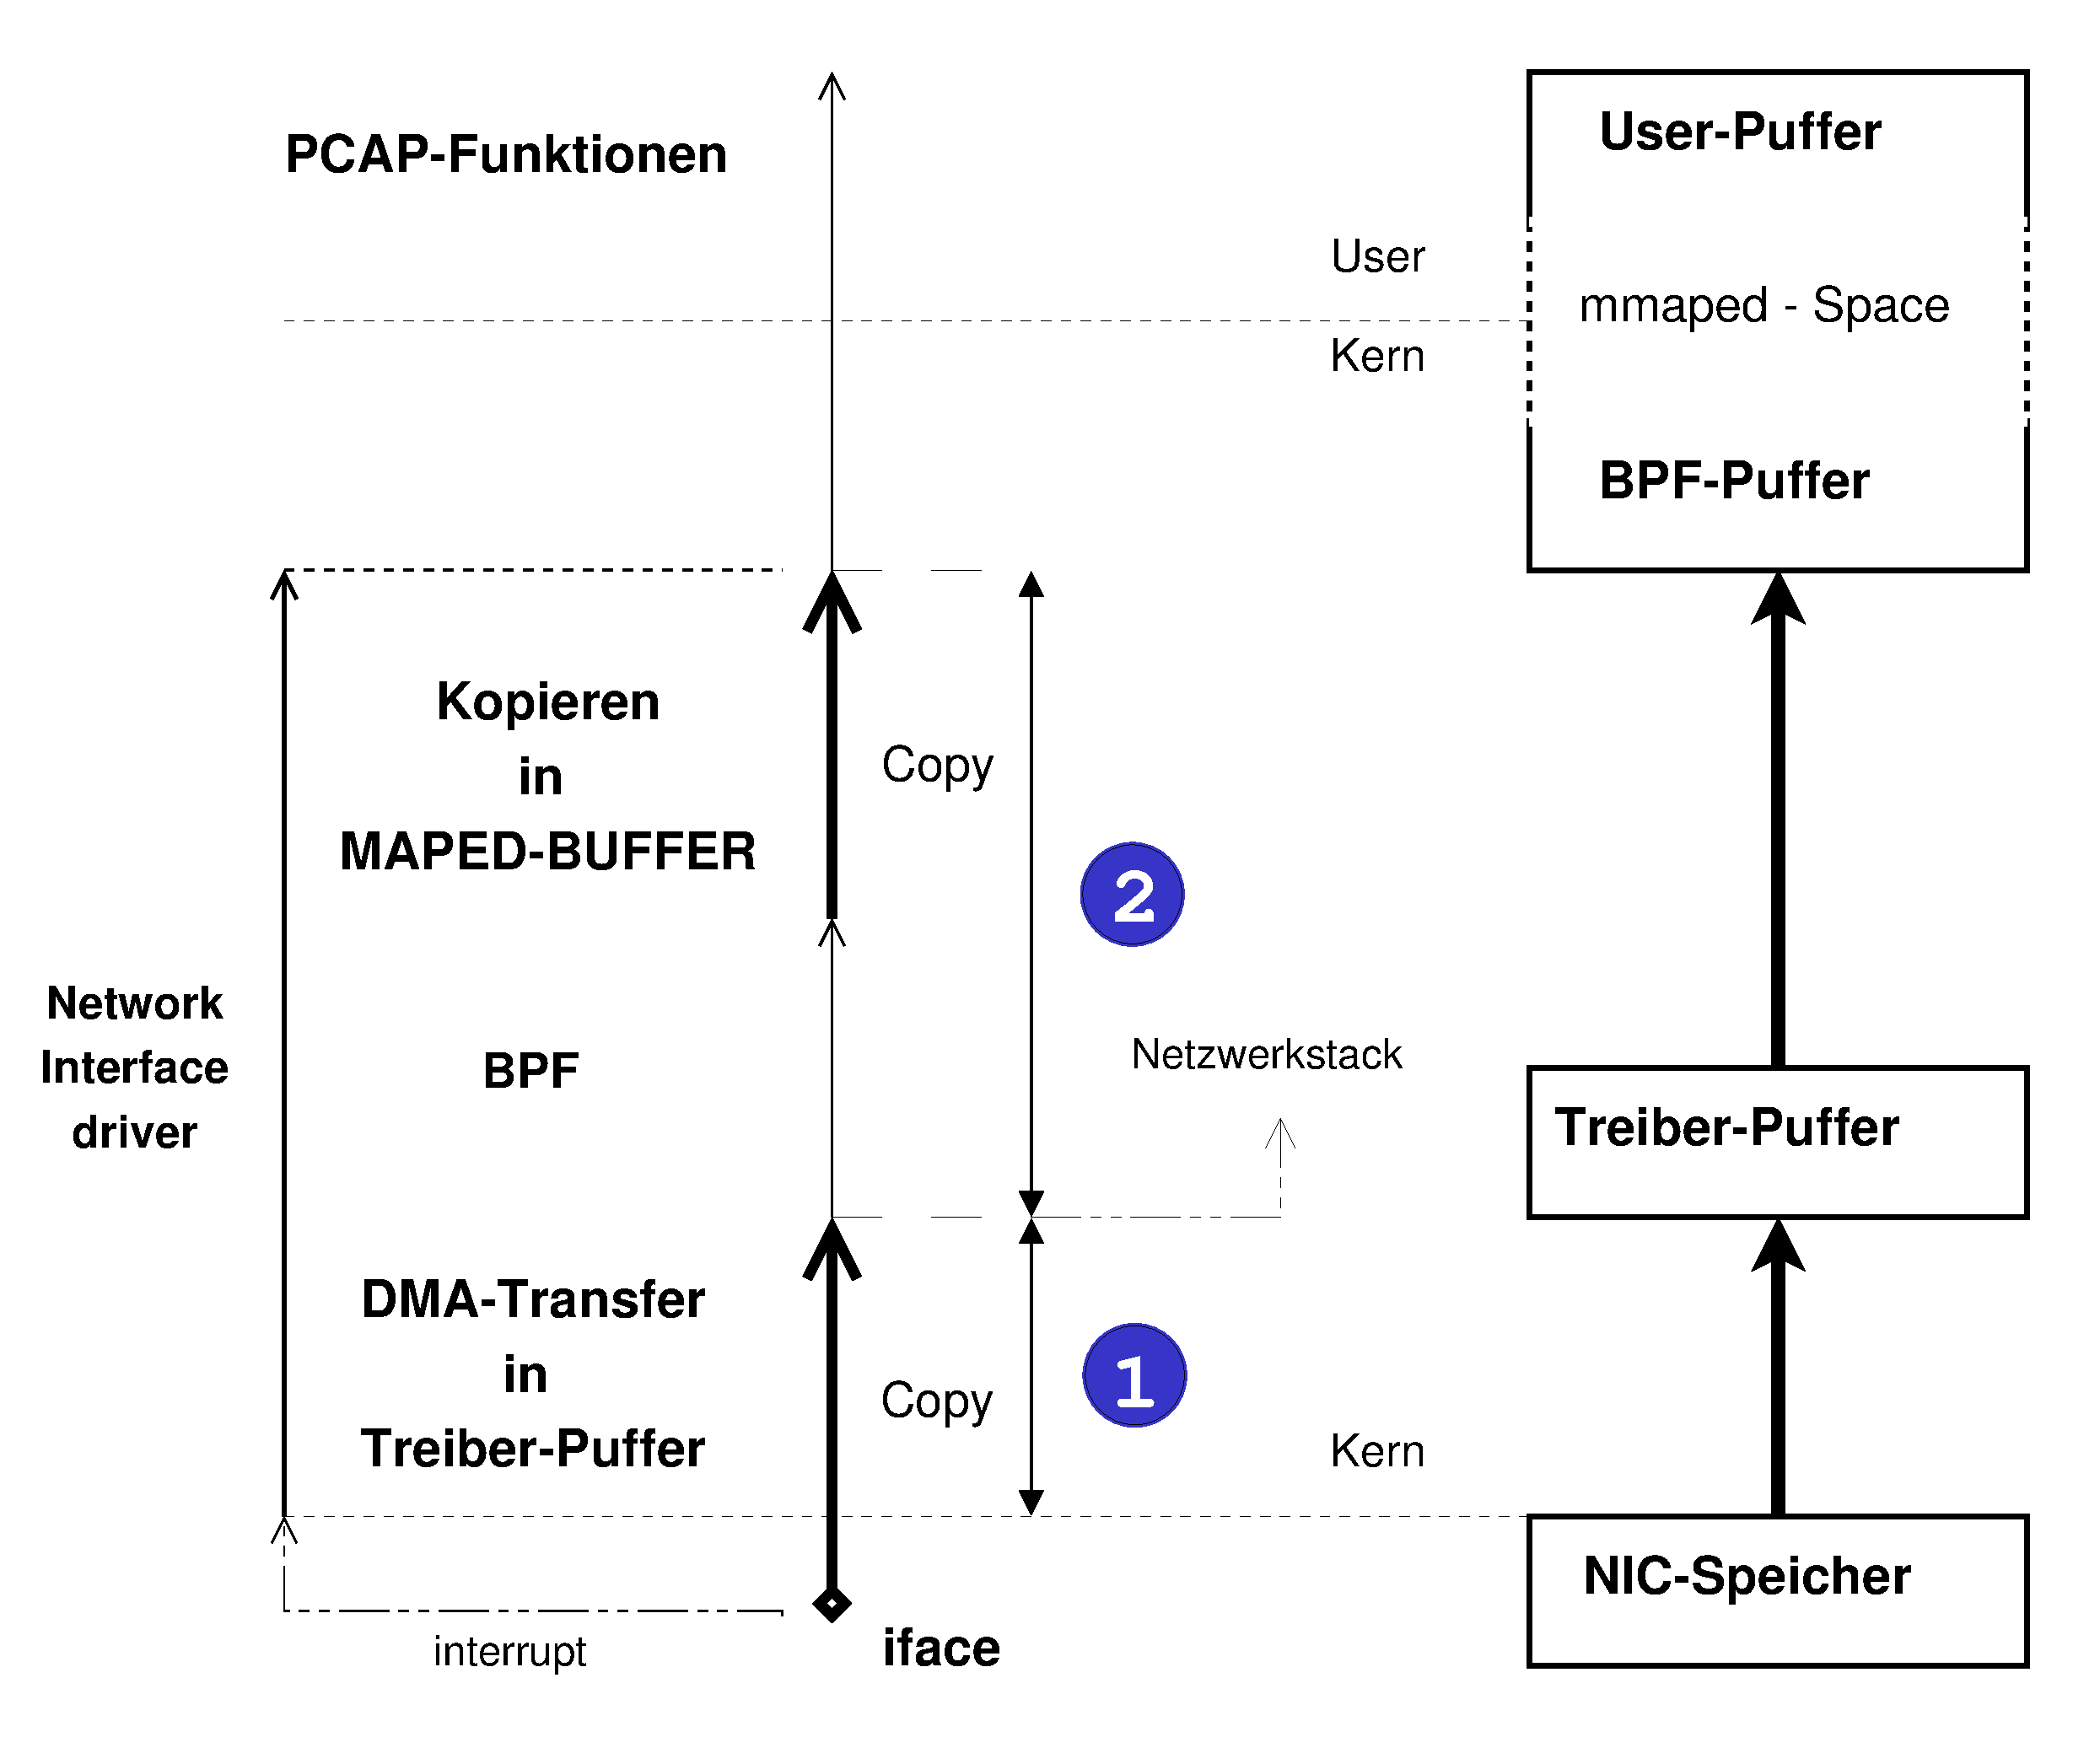
\includegraphics [width=1.00\textwidth, keepaspectratio]{pics/2copy}	
%	\end{columns}
%\end{frame}
%
%
%\begin{frame}
%\frametitle{Reduzieren der Anzahl von Copy-Operationen}
%		Beseitigen zwei Copy: Abbilden des Treiber-Puffers in User-Space \newline \\
%	\begin{columns}
%	\column[t]{0.5\textwidth}
%	\vspace{-10em}
%	\begin{enumerate}
%		\item Paketenempfang
%			\begin{itemize}
%				\item Datenkopieren:\newline NIC\textrightarrow RAM
%			\end{itemize}
%		\item Paketenauswerten und Filtern
%			\begin{itemize}
%				\item Auswerten und Filtern in User-Space
%				\item PCAP-BPF anwenden
%			\end{itemize}
%	\end{enumerate}
%	\column[t]{0.5\textwidth}
%	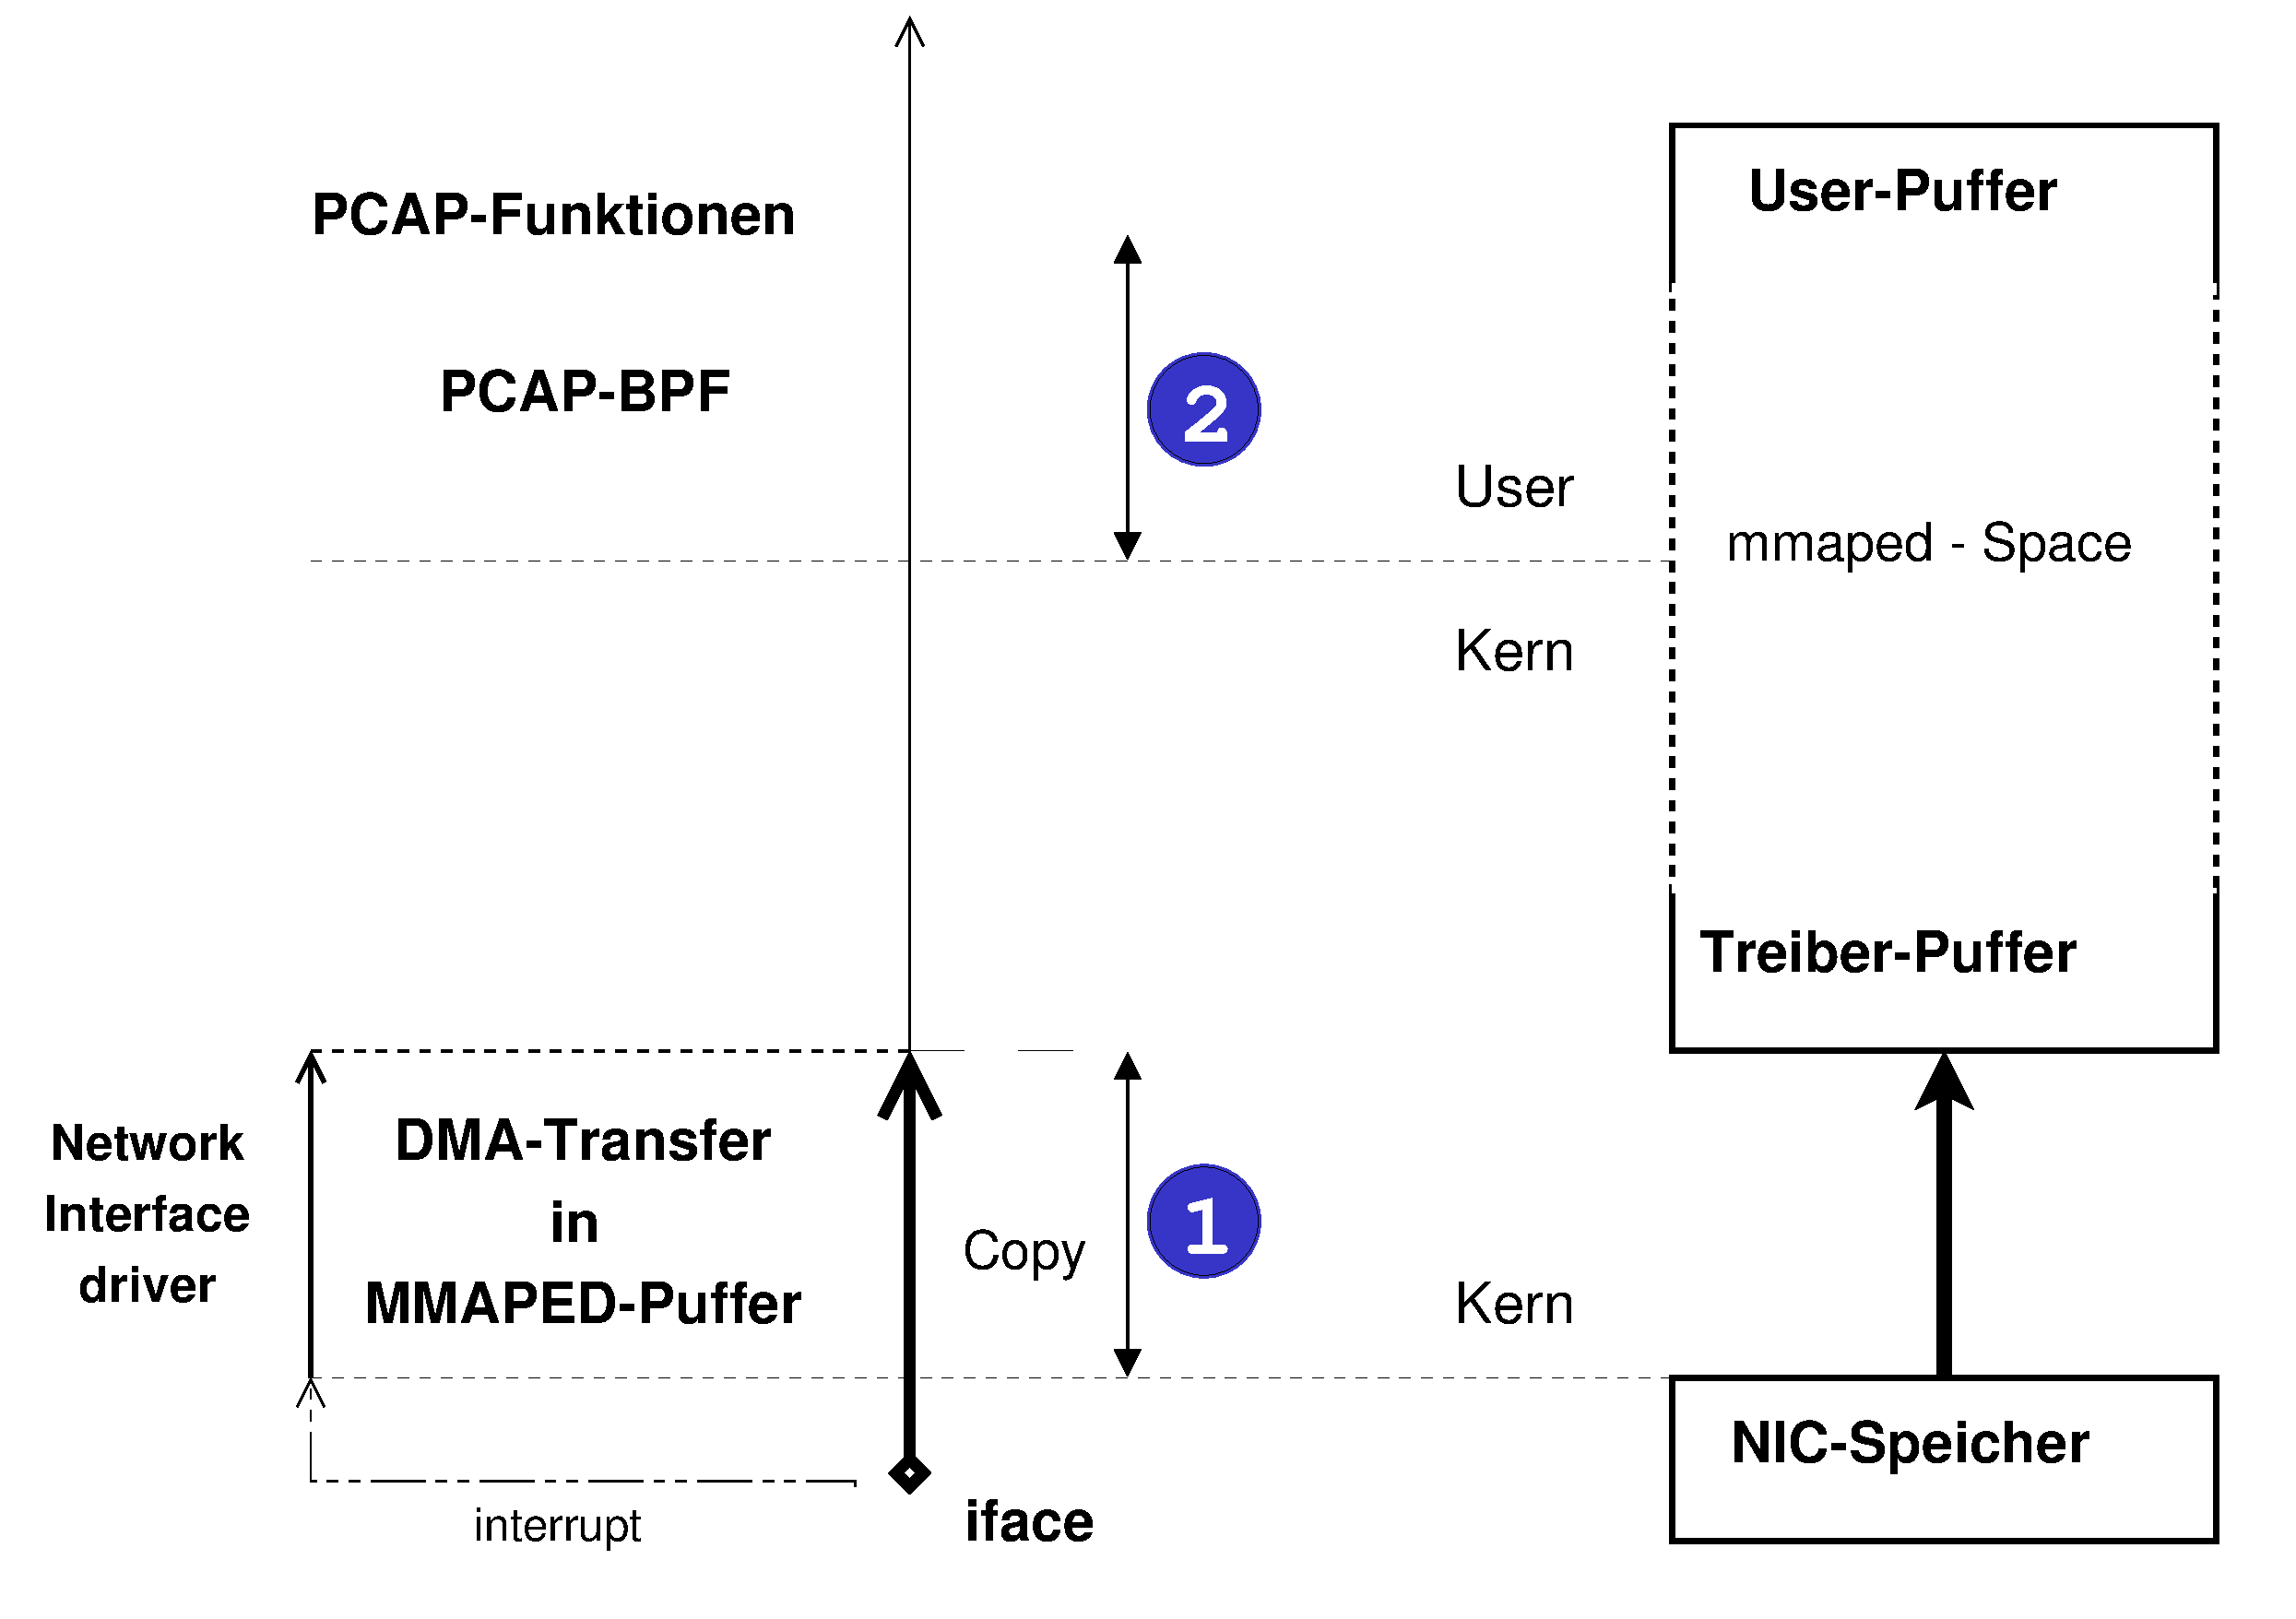
\includegraphics [width=1.00\textwidth, high=1.00\texthigh, keepaspectratio]{pics/1copy}
%	\end{columns}
%\end{frame}
%	
%
%\begin{frame}
%\frametitle{"Uberblick}
%\begin{columns}
%	\column[t]{0.4\textwidth}
%	\vspace{-16em}
%	\begin{itemize}
%		\item[\sffamily A.] Ausgangssituation 
%		\item[\sffamily B.] Mapping des BPF-Puffers in User-Space
%		\item[\sffamily C.] Mapping des Treiber-Puffers in User-Space
%			\begin{itemize}
%				\item Ausschalten des Protokolstacks
%				\item Auswerten und Filtern der Paketen in User-Space
%			\end{itemize}
%	\end{itemize}
%
%	\column[t]{0.6\textwidth}
%	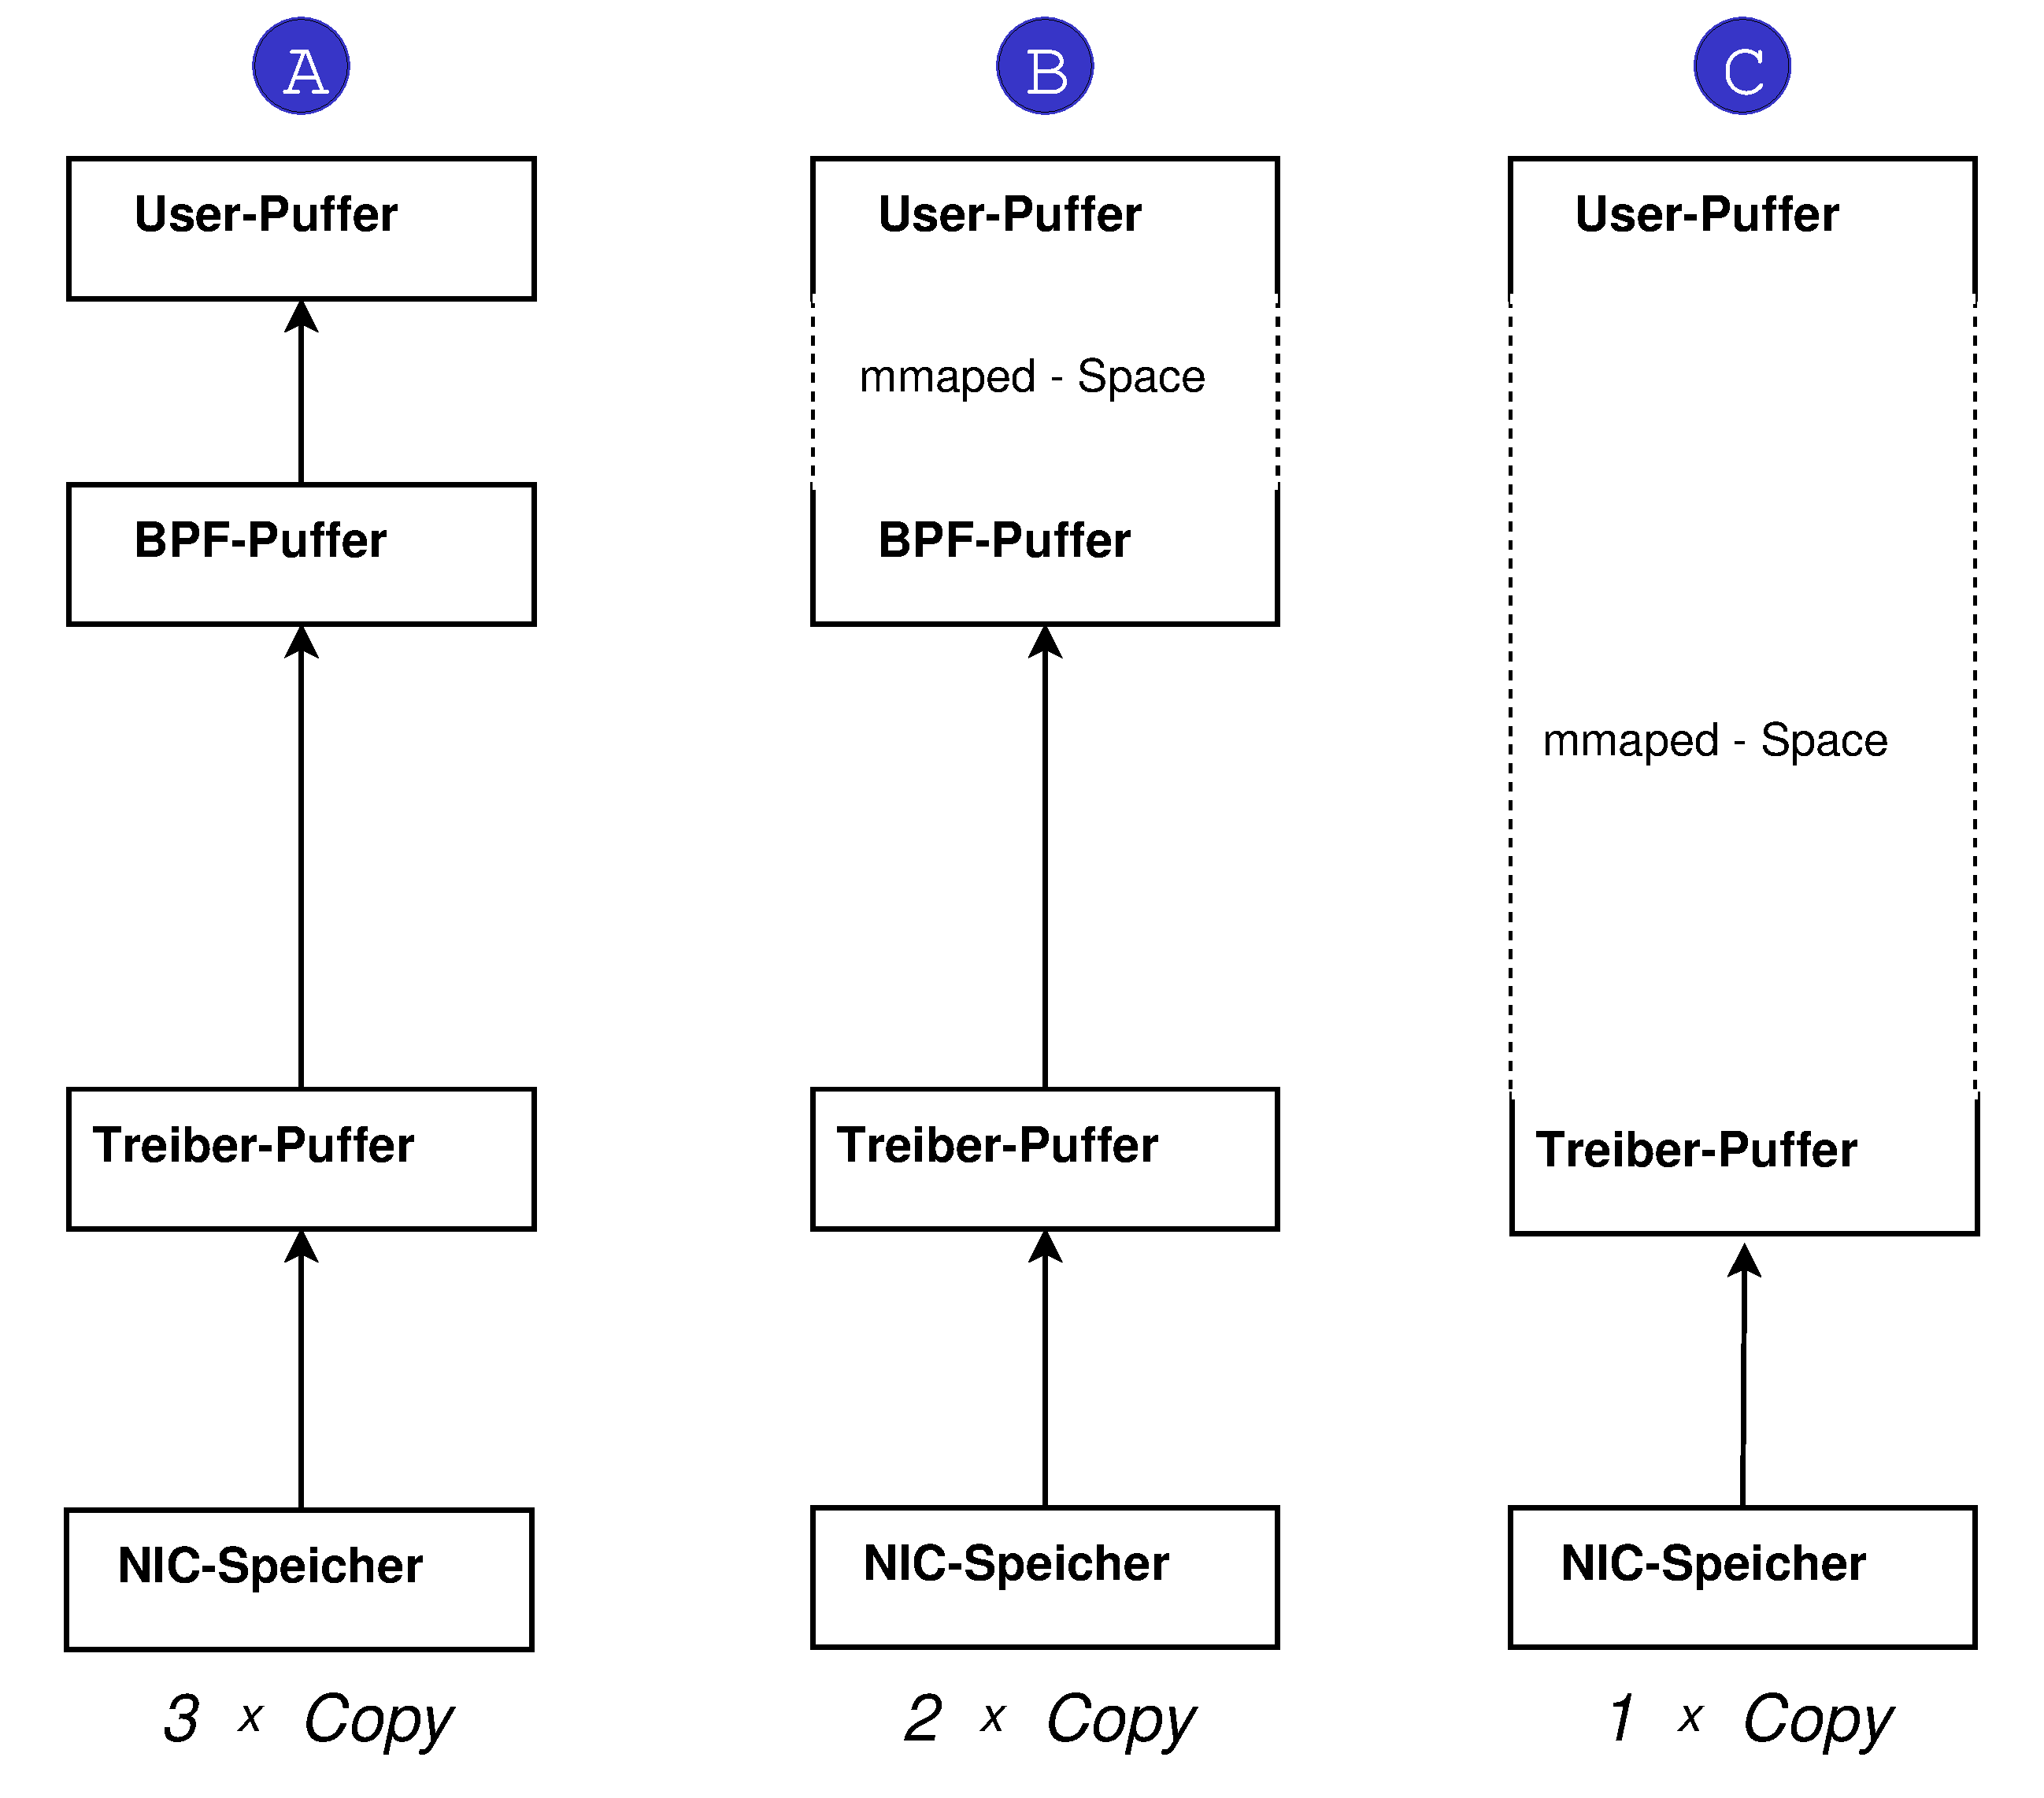
\includegraphics [width=1.00\textwidth, keepaspectratio]{pics/Overview}
%
%\end{columns}
%\end{frame}
%
%
%\begin{frame}
%\frametitle{Reduzieren von hohen Interrupt-Load}
%	\begin{itemize}
%		\item  	Das Timer-Driven Interrupt Modell
%			\begin{itemize}
%				\item Unterstz"utzung von Hardware notwendig
%			\end{itemize}
%		\item	Polling
%		\item	Prozessor-Affinity. SMP
%	\end{itemize}
%\end{frame}
%
%
%\begin{frame}
%\frametitle{Reduzieren von hohen Interrupt-Load}
%			Das Timer-Driven Interrupt Modell \newline \\
%\begin{itemize}
%	\item Realisiert in einigen Netzwerkkarten (z.B. Intel PRO*)
%	\item Sammeln von Interrupt-Ereignissen
%	\item Bearbeiten von mehreren Paketen in einem Interrupt
%\end{itemize}
%\end{frame}
%
%
%\begin{frame}
%\frametitle{Reduzieren von hohen Interrupt-Load}
%		Polling \newline \\
%			\begin{itemize}
%				\item Abfragen der Netzwerkger"aten in regelm"assigen Zeitintervallen 
%						nach vorhandenen Paketen
%				\item Wird "uber {\it sysctl kern.polling.*} konfiguriert
%					\begin{itemize}
%						\item {\it sysctl kern.polling.useri\_frac} -- stellt das Anteil 
%								der CPU-Zeit f"ur Benutzerprozesse
%				\item Fraglich, ob bei SMP einen Gewinn bringt
%					\end{itemize}
%			\end{itemize}
%\end{frame}
%
%
%\begin{frame}
%\frametitle{Reduzieren von hohen Interrupt-Load}
%Prozessor-Affinity. SMP \newline \\
%	\begin{itemize}
%	\item 	Interrupts und Paketbearbeitungsprozess auf verschiedenen 
%			CPUs (bzw. Cores) ausf"uhren
%	\item 	Programmable I/O anstatt DMA-Transfer 
%		\begin{itemize}
%			\item CPU bringt die Daten beim lesen aus Hardwareregistern in Cache
%			\item Der Prozess auf dem anderen CPU-Kern  holt die Daten 
%					aus dem Cache schneller
%			\item Macht, wahrscheinlich, Sinn nur auf SMP, weil bei 
%					NUMA werden die Daten im fremden Cache auftauchen
%			\begin{itemize}
%				\item Cache-Miss kann in dem Fall zu "`teuer"' sein 
%			\end{itemize}
%		\end{itemize}
%	\end{itemize}
%\end{frame}
%
%
%% Zusammenfassung
%\section {Zusammenfassung}
%\begin{frame}
%\frametitle{Zusammenfassung}
%	\begin{itemize}
%	\item Worum es geht 
%		\begin{itemize}
%			\item Capturing
%		\end{itemize}
%
%	\item Wo liegt das Problem
%		\begin{itemize}
%			\item Datenverlust beim Capturing
%		\end{itemize}
%	\item Ursachen
%		\begin{itemize}
%			\item Nicht ausreichende Datentransferrate der internen Bussen
%			\item Hohe Interrupt-Load
%		\end{itemize}
%	\item L"osung
%		\begin{itemize}
%			\item Tuning von {\it sysctl - }Variablen um Polling bzw.
%					Timer-Driven zu optimieren
%			\item MMAP anstatt Copy
%			\item CPU-Affinity um Last zu verteilen
%
%		\end{itemize}
%	\end{itemize}
%\end{frame}
%
%
\end{document}
